%%%%%%%%%%%%%%%%%%%%%%%%%%%%% Thesis.tex %%%%%%%%%%%%%%%%%%%%%%%%%%%%%%%
%                                                                      %
%  ---------- Master of Science Dissertation template ----------       %
%                                                                      %
%  Template for the Master Thesis according to the regulations         %
%  published by the Academic Board (Direcção Académica) at IST.        %
%                                                                      %
%  For up-to-date guide, please refer to the official website          %
%  http://academica.tecnico.ulisboa.pt/alunos/dissertacao-de-mestrado/ %
%                                                                      %
%       Andre C. Marta                                                 %
%       Area Cientifica de Mecanica Aplicada e Aeroespacial            %
%       Departamento de Engenharia Mecanica                            %
%       Instituto Superior Tecnico                                     %
%       Av. Rovisco Pais                                               %
%       1049-001 Lisboa                                                %
%       Portugal                                                       %
%       Tel: +351 21 841 9469                                          %
%                        3469 (extension)                              %
%       Email: andre.marta@tecnico.ulisboa.pt                          %
%                                                                      %
%  Created:       Jan 20, 2011                                         %
%  Last Modified: Feb 19, 2018                                         %
%                                                                      %
%%%%%%%%%%%%%%%%%%%%%%%%%%%%%%%%%%%%%%%%%%%%%%%%%%%%%%%%%%%%%%%%%%%%%%%%
%  Revision history                                                    %
%  v1 - 2011/01/24 - original template                                 %
%  v2 - 2012/10/30 - new IST image and glossary support                %
%  v3 - 2013/12/10 - update according to 2012/13 official guide        %
%  v4 - 2014/02/28 - new default for bibliography style                %
%  v5 - 2014/05/07 - update according to 2013/14 official guide        %
%  v6 - 2015/07/02 - cover page format fixed,                          %
%                    contents page numbering fixed,                    %
%                    better language support,                          %
%                    enhanced examples of tables,                      %
%                    new option for appendix page numbering format,    %
%                    custom bibliography style                         %
%  v7 - 2018/02/19 - multiple citations compressed                     %
%%%%%%%%%%%%%%%%%%%%%%%%%%%%%%%%%%%%%%%%%%%%%%%%%%%%%%%%%%%%%%%%%%%%%%%%
%                                                                      %
% To generate the PDF file, type "make" at the terminal prompt.        %
%                                                                      %
% The IST template LaTeX package was created by the author             %
% and it can be downloaded from:                                       %
% https://fenix.ist.utl.pt/homepage/ist31052/                          %
%                                                                      %
% The external packages can be downloaded from                         %
% the Comprehensive TeX Archive Network at http://www.ctan.org/        %
%                                                                      %
% List of LaTex symbols:                                               %
% http://www.ctan.org/tex-archive/info/symbols/comprehensive/          %
%                                                                      %
% Help with LaTex can be found at                                      %
% http://www.giss.nasa.gov/tools/latex/ltx-2.html                      %
% http://en.wikibooks.org/wiki/LaTeX                                   %
%%%%%%%%%%%%%%%%%%%%%%%%%%%%%%%%%%%%%%%%%%%%%%%%%%%%%%%%%%%%%%%%%%%%%%%%

%%%%%%%%%%%%%%%%%%%%%%%%%%%%%%%%%%%%%%%%%%%%%%%%%%%%%%%%%%%%%%%%%%%%%%%%
%     Preamble                                                         %
%%%%%%%%%%%%%%%%%%%%%%%%%%%%%%%%%%%%%%%%%%%%%%%%%%%%%%%%%%%%%%%%%%%%%%%%

% ----------------------------------------------------------------------
%  Set the document class
% ----------------------------------------------------------------------
\documentclass[10pt,a4paper,twoside]{report}

% ----------------------------------------------------------------------
% Define external packages, language, margins, fonts and new commands
% ----------------------------------------------------------------------
\usepackage{todonotes}
\usepackage{glossaries}
\usepackage{pgfplots}
\newacronym{ml}{ML}{Machine Learning}
\newacronym{pe}{PE}{Portable Executable}
\newacronym{dll}{DLL}{Dynamic-link Library}
\newacronym{nsrl}{NSRL}{National Software Reference Library}
\newacronym{roc}{ROC}{Receiver Operating Characteristic}
\newacronym{auroc}{AUROC}{Area Under the Receiver Operating Characteristic}
\newacronym{dr}{DR}{Detection Rate}
\newacronym{fpr}{FPR}{False Postive Rate}
\newacronym{tts}{TTS}{The Top Set}
\newacronym{tgs}{TGS}{The Good Set}
\newacronym{tbs}{TBS}{The Bad Set}
\newacronym{lr}{LR}{Logistic Regression}
\newacronym{hids}{HIDS}{Host-based Intrusion Detection Systems}
\newacronym{caro}{CARO}{Computer Antivirus Research Organization}
\newacronym{ai}{AI}{Artificial Intelligence}
\newacronym{api}{API}{Application Programming Interface}
\newacronym{bios}{BIOS}{Basic Input/Output System}
\newacronym{cc}{CC}{Creative Common's}
\newacronym{ann}{ANN}{Artificial Neural Networks}
\newacronym{tpr}{TPR}{True Positive Rate}
\newacronym{svm}{SVM}{Support Vector Machine}
\newacronym{mist}{MIST}{Malware Instruction Set}

\newcommand\ie{\emph{i.e.}}
\newcommand\eg{\emph{e.g.}}

\newcommand\say[1]{``#1''}

\newcommand\miss[1]{\textcolor{red}{#1}}
\newcommand\dups{{dups}}
\newcommand\acc{acc}
\newcommand\mal{\mathrm{Malware}}
\newcommand\good{\mathrm{Goodware}}

\newcommand\CC{\mathcal{C}}
\newcommand\DD{\mathcal{D}}
\newcommand\FF{\mathcal{F}}
\newcommand\DS{\mathcal{S}}
\newcommand\LR{\mathcal{LR}}
% \newcommand\Ss\{\mathcal{S}}
% \newcommand\Ddups{\mathcal{D}_\dups}
\newcommand\II{\mathcal{I}}
\newcommand\Pf{\mathcal{P}_{f}}
\newcommand\Pl{\mathcal{P}_{l}}
\newcommand\RR{\mathcal{R}}
\newcommand\VV{\mathcal{V}}
\newcommand\VVdups{\mathcal{V}^{\dups}}
\newcommand\VVc{\mathcal{V}^{\CC}}
\newcommand\VVstar{\mathcal{V}^*}

\newcommand\tp{\textrm{TP}}
\newcommand\tn{\textrm{TN}}
\newcommand\fp{\textrm{FP}}
\newcommand\fn{\textrm{FN}}
\newcommand\dr{\textrm{DR}}
\newcommand\tpr{\textrm{TPR}}
\newcommand\tnr{\textrm{TNR}}
\newcommand\fpr{\textrm{FPR}}
\newcommand\fnr{\textrm{FNR}}

\newcommand\Madups{\mathcal{M}_{\acc}^{\dups}}
\newcommand\Mac{\mathcal{M}_{\acc}^{\CC}}
\newcommand\real{\mathrm{real}}
\newcommand\loose{\mathrm{loose}}
\newcommand\strict{\mathrm{strict}}
\newcommand\Mreal{\mathcal{M}_{\real}}
\newcommand\Mrealv{\mathcal{M}_{\real}^{\VVstar}}
\newcommand\Mloose{\mathcal{M}_{\loose}}
\newcommand\Mloosev{\mathcal{M}_{\loose}^{\VVstar}}
\newcommand\Mstrict{\mathcal{M}_{\strict}}
\newcommand\Mstrictv{\mathcal{M}_{\strict}^{\VVstar}}

\newcommand\NSRL{\mathrm{NSRL}}
\newcommand\VS{\mathrm{VS}}
\newcommand\CNSRL{\CC_{\NSRL}}
\newcommand\CVS{\CC_{\VS}}

%%%%%%%%%%%%%%%%%%%%%%%%%%%%%%%%%%%%%%%%%%%%%%%%%%%%%%%%%%%%%%%%%%%%%%%%
%                                                                      %
%     File: Thesis_Preamble.tex                                        %
%     Tex Master: Thesis.tex                                           %
%                                                                      %
%     Author: Andre C. Marta                                           %
%     Last modified : 9 Apr 2015                                       %
%                                                                      %
%%%%%%%%%%%%%%%%%%%%%%%%%%%%%%%%%%%%%%%%%%%%%%%%%%%%%%%%%%%%%%%%%%%%%%%%

% ----------------------------------------------------------------------
% Define document language.
% ----------------------------------------------------------------------

% 'inputenc' package
%
% Accept different input encodings.
% http://www.ctan.org/tex-archive/macros/latex/base/
%
% > allows typing non-english text in LaTeX sources.
%
% ******************************* SELECT *******************************
%\usepackage[latin1]{inputenc} % <<<<< Windows
\usepackage[utf8]{inputenc}   % <<<<< Linux
% ******************************* SELECT *******************************


% 'babel' package
%
% Multilingual support for Plain TeX or LaTeX.
% http://www.ctan.org/tex-archive/macros/latex/required/babel/
%
% > sets the variable names according to the language selected
%
% ******************************* SELECT *******************************
%\usepackage[portuguese]{babel} % <<<<< Portuguese
\usepackage[english]{babel} % <<<<< English
% ******************************* SELECT *******************************


% List of LaTeX variable names: \abstractname, \appendixname, \bibname,
%   \chaptername, \contentsname, \listfigurename, \listtablename, ...)
% http://www.tex.ac.uk/cgi-bin/texfaq2html?label=fixnam
%
% Changing the words babel uses (uncomment and redefine as necessary...)
%
\newcommand{\acknowledgments}{@undefined} % new LaTeX variable name
%
% > English
%
\addto\captionsenglish{\renewcommand{\acknowledgments}{Acknowledgments}}
%\addto\captionsenglish{\renewcommand{\contentsname}{Contents}}
%\addto\captionsenglish{\renewcommand{\listtablename}{List of Tables}}
%\addto\captionsenglish{\renewcommand{\listfigurename}{List of Figures}}
%\addto\captionsenglish{\renewcommand{\nomname}{Nomenclature}}
%\addto\captionsenglish{\renewcommand{\glossaryname}{Glossary}}
%\addto\captionsenglish{\renewcommand{\acronymname}{List of Acronyms}}
%\addto\captionsenglish{\renewcommand{\bibname}{References}} % Bibliography
%\addto\captionsenglish{\renewcommand{\appendixname}{Appendix}}

% > Portuguese
%
\addto\captionsportuguese{\renewcommand{\acknowledgments}{Agradecimentos}}
%\addto\captionsportuguese{\renewcommand{\contentsname}{Conte\'{u}do}}
%\addto\captionsportuguese{\renewcommand{\listtablename}{Lista de Figuras}}
%\addto\captionsportuguese{\renewcommand{\listfigurename}{Lista de Tabelas}}
\addto\captionsportuguese{\renewcommand{\nomname}{Lista de S\'{i}mbolos}} % Nomenclatura
%\addto\captionsportuguese{\renewcommand{\glossary}{Gloss\'{a}rio}}
%\addto\captionsportuguese{\renewcommand{\acronymname}{Lista de Abrevia\c{c}\~{o}es}}
%\addto\captionsportuguese{\renewcommand{\bibname}{Refer\^{e}ncias}} % Bibliografia
%\addto\captionsportuguese{\renewcommand{\appendixname}{Anexo}} % Apendice


% ----------------------------------------------------------------------
% Define cover fields in both english and portuguese.
% ----------------------------------------------------------------------
%
\newcommand{\coverThesis}{@undefined} % new LaTeX variable name
\newcommand{\coverSupervisors}{@undefined} % new LaTeX variable name
\newcommand{\coverExaminationCommittee}{@undefined} % new LaTeX variable name
\newcommand{\coverChairperson}{@undefined} % new LaTeX variable name
\newcommand{\coverSupervisor}{@undefined} % new LaTeX variable name
\newcommand{\coverMemberCommittee}{@undefined} % new LaTeX variable name
% > English
\addto\captionsenglish{\renewcommand{\coverThesis}{Thesis to obtain the Master of Science Degree in}}
\addto\captionsenglish{\renewcommand{\coverSupervisors}{Supervisor(s)}}
\addto\captionsenglish{\renewcommand{\coverExaminationCommittee}{Examination Committee}}
\addto\captionsenglish{\renewcommand{\coverChairperson}{Chairperson}}
\addto\captionsenglish{\renewcommand{\coverSupervisor}{Supervisor}}
\addto\captionsenglish{\renewcommand{\coverMemberCommittee}{Member of the Committee}}
% > Portuguese
\addto\captionsportuguese{\renewcommand{\coverThesis}{Disserta\c{c}\~{a}o para obten\c{c}\~{a}o do Grau de Mestre em}}
\addto\captionsportuguese{\renewcommand{\coverSupervisors}{Orientador(es)}}
\addto\captionsportuguese{\renewcommand{\coverExaminationCommittee}{J\'{u}ri}}
\addto\captionsportuguese{\renewcommand{\coverChairperson}{Presidente}}
\addto\captionsportuguese{\renewcommand{\coverSupervisor}{Orientador}}
\addto\captionsportuguese{\renewcommand{\coverMemberCommittee}{Vogal}}


% ----------------------------------------------------------------------
% Define default and cover page fonts.
% ----------------------------------------------------------------------

% Use Arial font as default
%
\renewcommand{\rmdefault}{phv}
\renewcommand{\sfdefault}{phv}

% Define cover page fonts
%
%         encoding     family       series      shape
%  \usefont{T1}     {phv}=helvetica  {b}=bold    {n}=normal
%                   {ptm}=times      {m}=normal  {sl}=slanted
%                                                {it}=italic
% see more examples at
% http://julien.coron.free.fr/languages/latex/fonts/
%
\def\FontLn{% 16 pt normal
  \usefont{T1}{phv}{m}{n}\fontsize{16pt}{16pt}\selectfont}
\def\FontLb{% 16 pt bold
  \usefont{T1}{phv}{b}{n}\fontsize{16pt}{16pt}\selectfont}
\def\FontMn{% 14 pt normal
  \usefont{T1}{phv}{m}{n}\fontsize{14pt}{14pt}\selectfont}
\def\FontMb{% 14 pt bold
  \usefont{T1}{phv}{b}{n}\fontsize{14pt}{14pt}\selectfont}
\def\FontSn{% 12 pt normal
  \usefont{T1}{phv}{m}{n}\fontsize{12pt}{12pt}\selectfont}


% ----------------------------------------------------------------------
% Define page margins and line spacing.
% ----------------------------------------------------------------------

% 'geometry' package
%
% Flexible and complete interface to document dimensions.
% http://www.ctan.org/tex-archive/macros/latex/contrib/geometry/
%
% > set the page margins (2.5cm minimum in every side, as per IST rules)
%
\usepackage{geometry}	
\geometry{verbose,tmargin=2.5cm,bmargin=2.5cm,lmargin=2.5cm,rmargin=2.5cm}

% 'setspace' package
%
% Set space between lines.
% http://www.ctan.org/tex-archive/macros/latex/contrib/setspace/
%
% > allow setting line spacing (line spacing of 1.5, as per IST rules)
%
\usepackage{setspace}
\renewcommand{\baselinestretch}{1.5}


% ----------------------------------------------------------------------
% Include external packages.
% Note that not all of these packages may be available on all system
% installations. If necessary, include the .sty files locally in
% the <jobname>.tex file directory.
% ----------------------------------------------------------------------

% 'graphicx' package
%
% Enhanced support for graphics.
% http://www.ctan.org/tex-archive/macros/latex/required/graphics/
%
% > extends arguments of the \includegraphics command
%
\usepackage{graphicx}


% 'color' package
%
% Colour control for LaTeX documents.
% http://www.ctan.org/tex-archive/macros/latex/required/graphics/
%
% > defines color macros: \color{<color name>}
%
%\usepackage{color}


% 'amsmath' package
%
% Mathematical enhancements for LaTeX.
% http://www.ctan.org/tex-archive/macros/latex/required/amslatex/
%
% > American Mathematical Society plain Tex macros
%
\usepackage{amsmath}  % AMS mathematical facilities for LaTeX.
\usepackage{amsthm}   % Typesetting theorems (AMS style).
\usepackage{amsfonts} % 


% 'wrapfig' package
%
% Produces figures which text can flow around.
% http://www.ctan.org/tex-archive/macros/latex/contrib/wrapfig/
%
% > wrap figures/tables in text (i.e., Di Vinci style)
%
% \usepackage{wrapfig}


% 'subfigure' package
%
% Deprecated: Figures divided into subfigures.
% http://www.ctan.org/tex-archive/obsolete/macros/latex/contrib/subfigure/
%
% > subcaptions for subfigures
%
\usepackage{subfigure}


% 'subfigmat' package
%
% Automates layout when using the subfigure package.
% http://www.ctan.org/tex-archive/macros/latex/contrib/subfigmat/
%
% > matrices of similar subfigures
%
\usepackage{subfigmat}


% 'url' package
%
% Verbatim with URL-sensitive line breaks.
% http://www.ctan.org/tex-archive/macros/latex/contrib/url/
%
% > URLs in BibTex
%
% \usepackage{url}


% 'varioref' package
%
% Intelligent page references.
% http://www.ctan.org/tex-archive/macros/latex/required/tools/
%
% > smart page, figure, table and equation referencing
%
%\usepackage{varioref}


% 'dcolumn' package
%
% Align on the decimal point of numbers in tabular columns.
% http://www.ctan.org/tex-archive/macros/latex/required/tools/
%
% > decimal-aligned tabular math columns
%
\usepackage{dcolumn}
\newcolumntype{d}{D{.}{.}{-1}} % column aligned by the point separator '.'
\newcolumntype{e}{D{E}{E}{-1}} % column aligned by the exponent 'E'


% 'verbatim' package
%
% Reimplementation of and extensions to LaTeX verbatim.
% http://www.ctan.org/tex-archive/macros/latex/required/tools/
%
% > provides the verbatim environment (\begin{verbatim},\end{verbatim})
%   and a comment environment (\begin{comment},  \end{comment})
%
% \usepackage{verbatim}


% 'moreverb' package
%
% Extended verbatim.
% http://www.ctan.org/tex-archive/macros/latex/contrib/moreverb/
%
% > supports tab expansion and line numbering
%
% \usepackage{moreverb}



% 'nomencl' package
%
% Produce lists of symbols as in nomenclature.
% http://www.ctan.org/tex-archive/macros/latex/contrib/nomencl/
%
% The nomencl package makes use of the MakeIndex program
% in order to produce the nomenclature list.
%
% Nomenclature
% 1) On running the file through LATEX, the command \makenomenclature
%    in the preamble instructs it to create/open the nomenclature file
%    <jobname>.nlo corresponding to the LATEX file <jobname>.tex and
%    writes the information from the \nomenclature commands to this file.
% 2) The next step is to invoke MakeIndex in order to produce the
%    <jobname>.nls file. This can be achieved by making use of the
%    command: makeindex <jobname>.nlo -s nomencl.ist -o <jobname>.nls
% 3) The last step is to invoke LATEX on the <jobname>.tex file once
%    more. There, the \printnomenclature in the document will input the
%    <jobname>.nls file and process it according to the given options.
%
% http://www-h.eng.cam.ac.uk/help/tpl/textprocessing/nomencl.pdf
%
% Nomenclature (produces *.nlo *.nls files)
\usepackage{nomencl}
\makenomenclature
%
% Group variables according to their symbol type
%
\RequirePackage{ifthen} 
\ifthenelse{\equal{\languagename}{english}}%
    { % English
    \renewcommand{\nomgroup}[1]{%
      \ifthenelse{\equal{#1}{R}}{%
        \item[\textbf{Roman symbols}]}{%
        \ifthenelse{\equal{#1}{G}}{%
          \item[\textbf{Greek symbols}]}{%
          \ifthenelse{\equal{#1}{S}}{%
            \item[\textbf{Subscripts}]}{%
            \ifthenelse{\equal{#1}{T}}{%
              \item[\textbf{Superscripts}]}{}}}}}%
    }{% Portuguese
    \renewcommand{\nomgroup}[1]{%
      \ifthenelse{\equal{#1}{R}}{%
        \item[\textbf{Simbolos romanos}]}{%
        \ifthenelse{\equal{#1}{G}}{%
          \item[\textbf{Simbolos gregos}]}{%
          \ifthenelse{\equal{#1}{S}}{%
            \item[\textbf{Subscritos}]}{%
            \ifthenelse{\equal{#1}{T}}{%
              \item[\textbf{Sobrescritos}]}{}}}}}%
    }%


% 'glossary' package
%
% Create a glossary.
% http://www.ctan.org/tex-archive/macros/latex/contrib/glossary/
%
% Glossary (produces *.glo *.ist files)
\usepackage[number=none]{glossary}
% (remove blank line between groups)
\setglossary{gloskip={}}
% (redefine glossary style file)
%\renewcommand{\istfilename}{myGlossaryStyle.ist}
\makeglossary


% 'rotating' package
%
% Rotation tools, including rotated full-page floats.
% http://www.ctan.org/tex-archive/macros/latex/contrib/rotating/
%
% > show wide figures and tables in landscape format:
%   use \begin{sidewaystable} and \begin{sidewaysfigure}
%   instead of 'table' and 'figure', respectively.
%
\usepackage{rotating}


% 'hyperref' package
%
% Extensive support for hypertext in LaTeX.
% http://www.ctan.org/tex-archive/macros/latex/contrib/hyperref/
%
% > Extends the functionality of all the LATEX cross-referencing
%   commands (including the table of contents, bibliographies etc) to
%   produce \special commands which a driver can turn into hypertext
%   links; Also provides new commands to allow the user to write adhoc
%   hypertext links, including those to external documents and URLs.
%
\usepackage[pdftex]{hyperref} % enhance documents that are to be
                              % output as HTML and PDF
\hypersetup{colorlinks,       % color text of links and anchors,
                              % eliminates borders around links
%            linkcolor=red,    % color for normal internal links
            linkcolor=black,  % color for normal internal links
            anchorcolor=black,% color for anchor text
%            citecolor=green,  % color for bibliographical citations
            citecolor=black,  % color for bibliographical citations
%            filecolor=magenta,% color for URLs which open local files
            filecolor=black,  % color for URLs which open local files
%            menucolor=red,    % color for Acrobat menu items
            menucolor=black,  % color for Acrobat menu items
%            pagecolor=red,    % color for links to other pages
            pagecolor=black,  % color for links to other pages
%            urlcolor=cyan,    % color for linked URLs
            urlcolor=black,   % color for linked URLs
	          bookmarks=true,         % create PDF bookmarks
	          bookmarksopen=false,    % don't expand bookmarks
	          bookmarksnumbered=true, % number bookmarks
	          pdftitle={Thesis},
            pdfauthor={Andre C. Marta},
            pdfsubject={Thesis Title},
            pdfkeywords={Thesis Keywords},
            pdfstartview=FitV,
            pdfdisplaydoctitle=true}


% 'hypcap' package
%
% Adjusting the anchors of captions.
% http://www.ctan.org/tex-archive/macros/latex/contrib/oberdiek/
%
% > fixes the problem with hyperref, that links to floats points
%   below the caption and not at the beginning of the float.
%
\usepackage[figure,table]{hypcap}


% 'natbib' package
%
% Flexible bibliography support.
% http://www.ctan.org/tex-archive/macros/latex/contrib/natbib/
%
% > produce author-year style citations
%
% \citet  and \citep  for textual and parenthetical citations, respectively
% \citet* and \citep* that print the full author list, and not just the abbreviated one
% \citealt is the same as \citet but without parentheses. Similarly, \citealp is \citep without parentheses
% \citeauthor
% \citeyear
% \citeyearpar
%
%% natbib options can be provided when package is loaded \usepackage[options]{natbib}
%%
%% Following options are valid:
%%
%%   round  -  round parentheses are used (default)
%%   square -  square brackets are used   [option]
%%   curly  -  curly braces are used      {option}
%%   angle  -  angle brackets are used    <option>
%%   semicolon  -  multiple citations separated by semi-colon (default)
%%   colon  - same as semicolon, an earlier confusion
%%   comma  -  separated by comma
%%   authoryear - for author–year citations (default)
%%   numbers-  selects numerical citations
%%   super  -  numerical citations as superscripts, as in Nature
%%   sort   -  sorts multiple citations according to order in ref. list
%%   sort&compress   -  like sort, but also compresses numerical citations
%%   compress - compresses without sorting
%%
% ******************************* SELECT *******************************
%\usepackage{natbib}          % <<<<< References in alphabetical list Correia, Silva, ...
\usepackage[numbers,sort&compress]{natbib} % <<<<< References in numbered list [1],[2],...
% ******************************* SELECT *******************************


% 'notoccite' package
%
% Prevent trouble from citations in table of contents, etc.
% http://ctan.org/pkg/notoccite
%
% > If you have \cite com­mands in \sec­tion-like com­mands, or in \cap­tion,
%   the ci­ta­tion will also ap­pear in the ta­ble of con­tents, or list of what­ever.
%   If you are also us­ing an un­srt-like bib­li­og­ra­phy style, these ci­ta­tions will
%   come at the very start of the bib­li­og­ra­phy, which is con­fus­ing. This pack­age
%   sup­presses the ef­fect.
%
\usepackage{notoccite}


% 'multirow' package
%
% Create tabular cells spanning multiple rows
% http://www.ctan.org/pkg/multirow
%
\usepackage{multirow}


% 'booktabs' package
%
% Publication quality tables in LaTeX
% http://www.ctan.org/pkg/booktabs
%
% > en­hance the qual­ity of ta­bles in LaTeX, pro­vid­ing ex­tra com­mands.
%
% \renewcommand{\arraystretch}{<ratio>} % space between rows
%
\usepackage{booktabs}
%\newcommand{\ra}[1]{\renewcommand{\arraystretch}{#1}}


% 'pdfpages' package
%
% Include PDF documents in LaTeX
% http://www.ctan.org/pkg/pdfpages
%
% > in­clu­sion of ex­ter­nal multi-page PDF doc­u­ments in LaTeX doc­u­ments.
%   Pages may be freely se­lected and sim­i­lar to psnup it is pos­si­ble to put
%   sev­eral log­i­cal pages onto each sheet of pa­per.
%
% \includepdf{filename.pdf}
% \includepdf[pages={4-9},nup=2x3,landscape=true]{filename.pdf}
%
\usepackage{pdfpages}


% ----------------------------------------------------------------------
% Define new commands to assure consistent treatment throughout document
% ----------------------------------------------------------------------

\newcommand{\ud}{\mathrm{d}}                % total derivative
\newcommand{\degree}{\ensuremath{^\circ\,}} % degrees

% Abbreviations

\newcommand{\mcol}{\multicolumn}            % table format

\newcommand{\eqnref}[1]{(\ref{#1})}
\newcommand{\class}[1]{\texttt{#1}}
\newcommand{\package}[1]{\texttt{#1}}
\newcommand{\file}[1]{\texttt{#1}}
\newcommand{\BibTeX}{\textsc{Bib}\TeX}

% Typefaces ( example: {\bf Bold text here} )
%
% > pre-defined
%   \bf % bold face
%   \it % italic
%   \tt % typewriter
%
% > newly defined
\newcommand{\tr}[1]{{\ensuremath{\textrm{#1}}}}   % text roman
\newcommand{\tb}[1]{{\ensuremath{\textbf{#1}}}}   % text bold face
\newcommand{\ti}[1]{{\ensuremath{\textit{#1}}}}   % text italic
\newcommand{\mc}[1]{{\ensuremath{\mathcal{#1}}}}  % math calygraphy
\newcommand{\mco}[1]{{\ensuremath{\mathcalold{#1}}}}% math old calygraphy
\newcommand{\mr}[1]{{\ensuremath{\mathrm{#1}}}}   % math roman
\newcommand{\mb}[1]{{\ensuremath{\mathbf{#1}}}}   % math bold face
\newcommand{\bs}[1]{\ensuremath{\boldsymbol{#1}}} % math symbol
\def\bm#1{\mathchoice                             % math bold
  {\mbox{\boldmath$\displaystyle#1$}}%
  {\mbox{\boldmath$#1$}}%
  {\mbox{\boldmath$\scriptstyle#1$}}%
  {\mbox{\boldmath$\scriptscriptstyle#1$}}}
\newcommand{\boldcal}[1]{{\ensuremath{\boldsymbol{\mathcal{#1}}}}}% math bold calygraphy

 % file "Thesis_Preamble.tex"

%%%%%%%%%%%%%%%%%%%%%%%%%%%%%%%%%%%%%%%%%%%%%%%%%%%%%%%%%%%%%%%%%%%%%%%%
%     Begin Document                                                   %
%%%%%%%%%%%%%%%%%%%%%%%%%%%%%%%%%%%%%%%%%%%%%%%%%%%%%%%%%%%%%%%%%%%%%%%%
\begin{document}

% Set plain page style (no headers, footer with centered page number)
\pagestyle{plain}

% Set roman numbering (i,ii,...) before the start of chapters
\pagenumbering{roman}

% ----------------------------------------------------------------------
%  Cover page
% ----------------------------------------------------------------------
%%%%%%%%%%%%%%%%%%%%%%%%%%%%%%%%%%%%%%%%%%%%%%%%%%%%%%%%%%%%%%%%%%%%%%%%
%                                                                      %
%     File: Thesis_FrontCover.tex                                      %
%     Tex Master: Thesis.tex                                           %
%                                                                      %
%     Author: Andre C. Marta                                           %
%     Last modified :  2 Jul 2015                                      %
%                                                                      %
%%%%%%%%%%%%%%%%%%%%%%%%%%%%%%%%%%%%%%%%%%%%%%%%%%%%%%%%%%%%%%%%%%%%%%%%

\thispagestyle {empty}

% IST Logo - Signature A
% parameters: bb=llx lly urx ury (bounding box), width=h_length, height=v_length, angle=angle, scale=factor, clip=true/false, draft=true/false. 
\includegraphics[bb=9.5cm 11cm 0cm 0cm,scale=0.29]{IST_A_CMYK_POS}

\begin{center}
%
% Figure (Image or plot)
% \vspace{2.5cm}
\vspace{5cm}
% height = 50 mm
% \includegraphics[height=50mm]{Figures/Airbus_A350.jpg}

% Title, author and degree
\vspace{1.0cm}
{\FontLb Malware Detection via Machine Learning} \\
%\vspace{0.2cm}
%{\FontMn Subtitle (optional)} \\
%\vspace{1.9cm}
\vspace{2.6cm}
{\FontMb João Carlos Fernandez Godinho} \\
\vspace{2.6cm}
{\FontSn \coverThesis} \\
\vspace{0.3cm}
{\FontLb Information Systems and Computer Engineering} \\
\vspace{1.5cm}
{\FontSn %
\begin{tabular}{ll}
 \coverSupervisor: & Prof. Pedro Miguel dos Santos Alves Madeira Adão \\

\end{tabular} } \\
\vspace{1.5cm}
{\FontMb \coverExaminationCommittee} \\
\vspace{0.5cm}
{\FontSn %
\begin{tabular}{c}
\coverChairperson:     Prof. Paolo Romano\\
\coverSupervisor:      Prof. Pedro Miguel dos Santos Alves Madeira Adão \\
\coverMemberCommittee: Prof. Miguel Nuno Dias Alves Pupo Correia
\end{tabular} } \\
\vspace{2cm}
{\FontMb June 2018} \\
%
\end{center}

 % file "Thesis_FrontCover.tex"
\cleardoublepage

% ----------------------------------------------------------------------
% Dedication page (optional)
% ----------------------------------------------------------------------
%%%%%%%%%%%%%%%%%%%%%%%%%%%%%%%%%%%%%%%%%%%%%%%%%%%%%%%%%%%%%%%%%%%%%%%%
%                                                                      %
%     File: Thesis_Dedication.tex                                      %
%     Tex Master: Thesis.tex                                           %
%                                                                      %
%     Author: Andre C. Marta                                           %
%     Last modified :  2 Jul 2015                                      %
%                                                                      %
%%%%%%%%%%%%%%%%%%%%%%%%%%%%%%%%%%%%%%%%%%%%%%%%%%%%%%%%%%%%%%%%%%%%%%%%

\null\vskip5cm%
\begin{flushright}
     Dedicated to someone special...
\end{flushright}
\vfill\newpage

 % file "Thesis_Dedication.tex"
\cleardoublepage

% ----------------------------------------------------------------------
%  Acknowledgments (optional)
% ----------------------------------------------------------------------
%%%%%%%%%%%%%%%%%%%%%%%%%%%%%%%%%%%%%%%%%%%%%%%%%%%%%%%%%%%%%%%%%%%%%%%%
%                                                                      %
%     File: Thesis_Acknowledgments.tex                                 %
%     Tex Master: Thesis.tex                                           %
%                                                                      %
%     Author: Andre C. Marta                                           %
%     Last modified :  2 Jul 2015                                      %
%                                                                      %
%%%%%%%%%%%%%%%%%%%%%%%%%%%%%%%%%%%%%%%%%%%%%%%%%%%%%%%%%%%%%%%%%%%%%%%%

\section*{\acknowledgments}

% Add entry in the table of contents as section
\addcontentsline{toc}{section}{\acknowledgments}

A few words about the university, financial support, research advisor, dissertation readers, faculty or other professors, lab mates, other friends and family...

 % file "Thesis_Acknowledgements.tex"
\cleardoublepage

% ----------------------------------------------------------------------
%  Abstract (both in English and Portuguese)
% ----------------------------------------------------------------------
% !TeX spellcheck = pt_PT
%%%%%%%%%%%%%%%%%%%%%%%%%%%%%%%%%%%%%%%%%%%%%%%%%%%%%%%%%%%%%%%%%%%%%%%%
%                                                                      %
%     File: Thesis_Resumo.tex                                          %
%     Tex Master: Thesis.tex                                           %
%                                                                      %
%     Author: João C. Godinho                                          %
%     Last modified :  May 2018                                        %
%                                                                      %
%%%%%%%%%%%%%%%%%%%%%%%%%%%%%%%%%%%%%%%%%%%%%%%%%%%%%%%%%%%%%%%%%%%%%%%%

\section*{Resumo}

% Add entry in the table of contents as section
\addcontentsline{toc}{section}{Resumo}

O uso de técnicas de aprendizagem supervisionada para a detecção de programas maliciosos tem sido cada vez mais utilizada para melhorar métodos clássicos de detecção.
Este trabalho desenvolveu um modelo para a detecção de programas maliciosos, analisou o impacto da confiabilidade dos dados de treino no resultado final do classificador, e definiu métricas para \textit{verdade absoluta}.
Para tal, desenvolvemos três cenários para conjuntos de dados, cujo conteúdo varia entre amostras inequivocamente maliciosas e legítimas para amostras mais ambíguas e reais.
Analisámos cada cenário em condições laboratoriais, onde metodologias padrão de validação cruzada são aplicadas, descartando a importância \textit{temporal} na detecção de programas maliciosos, e também em condições de mundo real, onde a dependência temporal é proposta e aplicada.
Além disso, modificámos o nosso modelo original de modo a possibilitar a extração de mais informação sobre uma amostra, ao implementar um modelo com multiplas camadas, e de maneira a melhorar os resultados finais, ao usar informação dinâmica sobre a amostras.
Usámos depois a nossa metodologia baseada na ordem temporal das amostras para reduzir o tamanho dos dados de treino sem comprometer resultados ótimos, concluindo que existe um número ideal de dados de treino, temporalmente consistentes com os dados de validação, tal que o resultado final é ótimo.
Finalmente, fornecemos aplicações práticas do nosso modelo ao implementar o serviço de detecção de programas maliciosos, que é também inserido num servidor de correio eletrónico para validar anexos.

\vfill

\textbf{\Large Palavras-chave:} Segurança, Aprendizagem Automática, Detecção de Programas Maliciosos, Consistência Temporal, Verdade Absoluta

   % file "Thesis_Resumo.tex"
\cleardoublepage

%%%%%%%%%%%%%%%%%%%%%%%%%%%%%%%%%%%%%%%%%%%%%%%%%%%%%%%%%%%%%%%%%%%%%%%%
%                                                                      %
%     File: Thesis_Abstract.tex                                        %
%     Tex Master: Thesis.tex                                           %
%                                                                      %
%     Author: João C. Godinho                                          %
%     Last modified :  May 2018                                        %
%                                                                      %
%%%%%%%%%%%%%%%%%%%%%%%%%%%%%%%%%%%%%%%%%%%%%%%%%%%%%%%%%%%%%%%%%%%%%%%%

\section*{Abstract}

% Add entry in the table of contents as section
\addcontentsline{toc}{section}{Abstract}

The use of supervised learning techniques for malware detection has been used increasingly to aid classical classification methods. 
In this work we aim at developing a malware detection model, analyzing the impact of the reliability of the training dataset on the final result of the classifier, and metrics to define the \emph{ground-truth}.
For this, we propose three datasets' scenarios whose content range from unambiguous malware and goodware samples to more ambiguous and real ones.
We analyze each scenario in laboratory conditions, where standard cross-validation methodologies are applied, discarding the importance of \emph{time} in malware detection, and also in real-world conditions, where temporal-based dependencies are proposed and applied.
Furthermore, we modify our original model to both enrich the extractable information, by implementing a multi layer model, and to improve the final results, by using dynamic information about the samples.
We then use our temporal-based methodologies to reduce the size of the training dataset without compromising optimal results, concluding that there exists an ideal number of necessary training folds, temporally consistent with the validation fold, that maximizes the overall score.
Finally, we provide practical applications of our model by implementing a malware detection service, which is also used in a email server pipeline to scan attachments.

\vfill

\textbf{\Large Keywords:} Security, Machine Learning, Malware Detection, Temporal Consistency, Ground Truth

 % file "Thesis_Abstract.tex"
\cleardoublepage

% ----------------------------------------------------------------------
%  Table of contents, list of tables, list of figures and nomenclature
% ----------------------------------------------------------------------

% Table of contents
%
\tableofcontents
\cleardoublepage 

% List of tables
%
% Add entry in the table of contents as section
\phantomsection
\addcontentsline{toc}{section}{\listtablename}
% Generate list
\listoftables
\cleardoublepage 

% List of figures
%
% Add entry in the table of contents as section
\phantomsection
\addcontentsline{toc}{section}{\listfigurename}
% Generate list
\listoffigures
\cleardoublepage 

% Nomenclature
%
% entries of nomenclature list
%%%%%%%%%%%%%%%%%%%%%%%%%%%%%%%%%%%%%%%%%%%%%%%%%%%%%%%%%%%%%%%%%%%%%%%%%
%                                                                      %
%     File: Thesis_Nomenclature.tex                                    %
%     Tex Master: Thesis.tex                                           %
%                                                                      %
%     Author: Andre C. Marta                                           %
%     Last modified : 21 Jan 2011                                      %
%                                                                      %
%%%%%%%%%%%%%%%%%%%%%%%%%%%%%%%%%%%%%%%%%%%%%%%%%%%%%%%%%%%%%%%%%%%%%%%%
%
% The definitions can be placed anywhere in the document body
% and their order is sorted by <symbol> automatically when
% calling makeindex in the makefile
%
% The \glossary command has the following syntax:
%
% \glossary{entry}
%
% The \nomenclature command has the following syntax:
%
% \nomenclature[<prefix>]{<symbol>}{<description>}
%
% where <prefix> is used for fine tuning the sort order,
% <symbol> is the symbol to be described, and <description> is
% the actual description.

% ----------------------------------------------------------------------
% Roman symbols [r]
%\nomenclature[ru]{$\bf u$}{Velocity vector.}
%\nomenclature[ru]{$u,v,w$}{Velocity Cartesian components.}
%\nomenclature[rp]{$p$}{Pressure.}
%\nomenclature[rC]{$C_D$}{Coefficient of drag.}
%\nomenclature[rC]{$C_L$}{Coefficient of lift.}
%\nomenclature[rC]{$C_M$}{Coefficient of moment.}
%
%% ----------------------------------------------------------------------
%% Greek symbols [g]
%\nomenclature[g]{$\rho$}{Density.}
%\nomenclature[g]{$\alpha$}{Angle of attack.}
%\nomenclature[g]{$\beta$}{Angle of side-slip.}
%\nomenclature[g]{$\mu$}{Molecular viscosity coefficient.}
%\nomenclature[g]{$\kappa$}{Thermal conductivity coefficient.}
%
%% ----------------------------------------------------------------------
%% Subscripts [s]
%\nomenclature[s]{$x,y,z$}{Cartesian components.}
%\nomenclature[s]{$i,j,k$}{Computational indexes.}
%\nomenclature[s]{$\infty$}{Free-stream condition.}
%\nomenclature[s]{ref}{Reference condition.}
%\nomenclature[s]{$n$}{Normal component.}
%
%% ----------------------------------------------------------------------
%% Supercripts [t]
%\nomenclature[t]{T}{Transpose.}
%\nomenclature[t]{*}{Adjoint.}

 % file "Thesis_Nomenclature.tex"
%
% Add entry in the table of contents as section
%\phantomsection
%\addcontentsline{toc}{section}{\nomname}
% Insert glossary/nomenclature section produced by MakeIndex
%\printnomenclature
%\cleardoublepage

% entries of glossary list
%%%%%%%%%%%%%%%%%%%%%%%%%%%%%%%%%%%%%%%%%%%%%%%%%%%%%%%%%%%%%%%%%%%%%%%%%
%                                                                      %
%     File: Thesis_Glossary.tex                                        %
%     Tex Master: Thesis.tex                                           %
%                                                                      %
%     Author: Andre C. Marta                                           %
%     Last modified : 30 Oct 2012                                      %
%                                                                      %
%%%%%%%%%%%%%%%%%%%%%%%%%%%%%%%%%%%%%%%%%%%%%%%%%%%%%%%%%%%%%%%%%%%%%%%%
%
% The definitions can be placed anywhere in the document body
% and their order is sorted by <symbol> automatically when
% calling makeindex in the makefile
%
% The \glossary command has the following syntax:
%
% \glossary{entry}
%
% The \nomenclature command has the following syntax:
%
% \nomenclature[<prefix>]{<symbol>}{<description>}
%
% where <prefix> is used for fine tuning the sort order,
% <symbol> is the symbol to be described, and <description> is
% the actual description.

% ----------------------------------------------------------------------

\glossary{name={\textbf{MDO}},description={Multi-Disciplinar Optimization is an engineering technique that uses optimization methods to solve design problems incorporating two or more disciplines.}}

\glossary{name={\textbf{CFD}},description={Computational Fluid Dynamics is a branch of fluid mechanics that uses numerical methods and algorithms to solve problems that involve fluid flows.}}

\glossary{name={\textbf{CSM}},description={Computational Structural Mechanics is a branch of structure mechanics that uses numerical methods and algorithms to perform the analysis of structures and its components.}}

 % file "Thesis_Glossary.tex"

% Add entry in the table of contents as section
%\phantomsection
%\addcontentsline{toc}{section}{\glossaryname}
% Insert glossary section produced by MakeIndex
%\printglossary
%\cleardoublepage

% Set arabic numbering (1,2,...) after preface
%
\setcounter{page}{1}
\pagenumbering{arabic}

% ----------------------------------------------------------------------
%  Chapters
% ----------------------------------------------------------------------

%%%%%%%%%%%%%%%%%%%%%%%%%%%%%%%%%%%%%%%%%%%%%%%%%%%%%%%%%%%%%%%%%%%%%%%%
%                                                                      %
%     File: Thesis_Introduction.tex                                    %
%     Tex Master: Thesis.tex                                           %
%                                                                      %
%     Author: Andre C. Marta                                           %
%     Last modified :  2 Jul 2015                                      %
%                                                                      %
%%%%%%%%%%%%%%%%%%%%%%%%%%%%%%%%%%%%%%%%%%%%%%%%%%%%%%%%%%%%%%%%%%%%%%%%

\chapter{Introduction}
\label{chapter:introduction}

The number of reported security breaches due to \emph{virus}, \emph{trojans}, \emph{ransomwares}, etc, has been growing considerably in recent years~\cite{av-test:report} with reports of infections due to \emph{malware}  making the headlines, now more than ever.
Almost every week one such security vulnerability is reported which may be seen as a failure by the security community on the control and detection of malicious content. 

Due to the significant number of malware attacks, and taking into consideration the increasing popularity and huge success of \gls{ml} methodologies in classification in different domains~\cite{lee2003learning,joachims2002learning,li2010object,ding2001multi}, it is only natural to see these techniques applied to complement classical methodologies for malicious-content detection~\cite{arp2014drebin,christodorescu:semantics,kolosnjaji2016deep,kolter:learning,miller:rev_int,nissim:al_pdf,perdisci:behavior,rieck:dynamic,santos2013opcode,schultz:data_mining,schwenk2012autonomous,vsrndic2013detection,deo2016prescience,gandotra2014malware,jordaney2017transcend,rossow:practices}, in particular, supervised learning techniques.

%%%%%%%%%%%%%%%%%%%%%%%%%%%%%%%%%%%%%%%%%%%%%%%%%%%%%%%%%%%%%%%%%%%%%%%%
\section{Motivation}
\label{section:motivation}

Malware, which can be referred to by other names like malicious software or malicious code, can be described as \say{any code added, changed, or removed from a software system in order to	intentionally cause harm or subvert the intended function of the system}~\cite{mcgraw:mal_code}.
Malware can be a piece of code attached to a legitimate program, an independent program, or a combination of both.

The reasoning that leads to malware creation varies greatly, some are created to demonstrate some vulnerability or concept and do not cause direct harm to systems, while others are used to steal information or render systems useless.
The wide variety and quantity of now-a-day systems and the amount of sensitive information they store provide numerous opportunities to illegally make a profit out of subverting legitimate systems.

The amount of malware has shown an exponential increase since the early 2000s, from 1 million in 2006 to over 500 million by the end of 2016~\cite{av-test:report,mcafee:report}. According to a 2007 study by McAfee\footnote{McAfee Study Finds 4 Percent of Search Results Malicious, by Frederick Lane, June 4, 2007 [http://www.newsfactor.com/story.xhtml?story\_id=010000CEUEQO]} about 4\% of the query results by major search engines lead to potentially dangerous websites. A more recent study by Norton in 2010\footnote{Symantec Press Release, July 29, 2010 [https://www.symantec.com/en/aa/about/newsroom/press-releases/2010/symantec\_0729\_02]} showed that at least 10\% of top trending search terms returned malicious results. From the contact with malicious software, 1.1 billion identities (\ie\ user's personal information) have been exposed in 2016 alone~\cite{symantec:report}.

To detect malicious software, anti-virus solutions rely on two main methods: \textit{signature-based}, which uses a database of known malware to detect malware and \textit{heuristic-based}, which make use of malicious patterns and sets of rules to detect both known and new malware~\cite{gryaznov:scanners}.

To help in the task of detecting both new and old malware, the use of \gls{ml} methodologies have shown promising results~\cite{arp2014drebin,christodorescu:semantics,kolosnjaji2016deep,kolter:learning,miller:rev_int,nissim:al_pdf,perdisci:behavior,rieck:dynamic,santos2013opcode,schultz:data_mining,schwenk2012autonomous,vsrndic2013detection} when dealing with this task, but not without its pitfalls~\cite{deo2016prescience,gandotra2014malware,jordaney2017transcend,rossow:practices}.

The very first pitfall is the definition of \textit{malware}, not only the lack of an agreed upon definition brings the problem of having different anti-virus vendors classifying the same program differently, but also some programs fall within a gray area for which no clear classification can be deemed correct.
An example is what is called \textit{adware}, advertising-supported software, that although not performing directly malicious actions, perform arguably non-requested actions.
The non-existence of concrete metrics and properties that uniquely distinguish malware from goodware requires an extra effort in the preparation of datasets for evaluation of malware detectors.

Other problematic when using \gls{ml} for malware detection is how to evaluate the trained model.
While many classification tasks are time independent, one might argue that malware detection is not.
As such, applying common evaluation strategies that disregard for any temporal consistency affects the model performance~\cite{deo2016prescience,jordaney2017transcend,rossow:practices}.


%%%%%%%%%%%%%%%%%%%%%%%%%%%%%%%%%%%%%%%%%%%%%%%%%%%%%%%%%%%%%%%%%%%%%%%%
\section{Main Goal}
\label{section:overview}

The \acrfull{ml} field studies the development of computer programs that improve with experience.
A program is given a task and an experience, if its performance at the task improves with the experience given, then the program is learning the task~\cite{mitchell:ml}.

In this work we took advantage of \gls{ml} capabilities and the growing number of malware samples to investigate how one can develop a model that takes into account the aforementioned pitfalls.

To achieve this, we took an incremental approach to build a malware detection model, enabling us to measure the impacts of \textit{ground-truth} (\ie\ the gray area when it comes to malware), as well as how enforcing temporal consistent learning influences the final results.

To achieve our \textit{ground-truth} impact objective we made a comparative analysis of a supervised learning approach in three different scenarios (depicted in Figure~\ref{fig:scenarios}): 

\begin{itemize}
	\item \emph{strict scenario} where only very well-characterized samples are considered;
	\item \emph{loose scenario} where a wider set of still well-studied samples is considered;
	\item \emph{realistic scenario} where we get closer to the reality faced by vendors of malware detection solutions.
\end{itemize}

By designing these three scenarios, we can better understand how having a smaller and very distinctive dataset compares to a bigger and more uneven dataset, providing a greater understanding of the effects of \textit{ground-truth}.


\begin{figure}[!h]
	\centering
	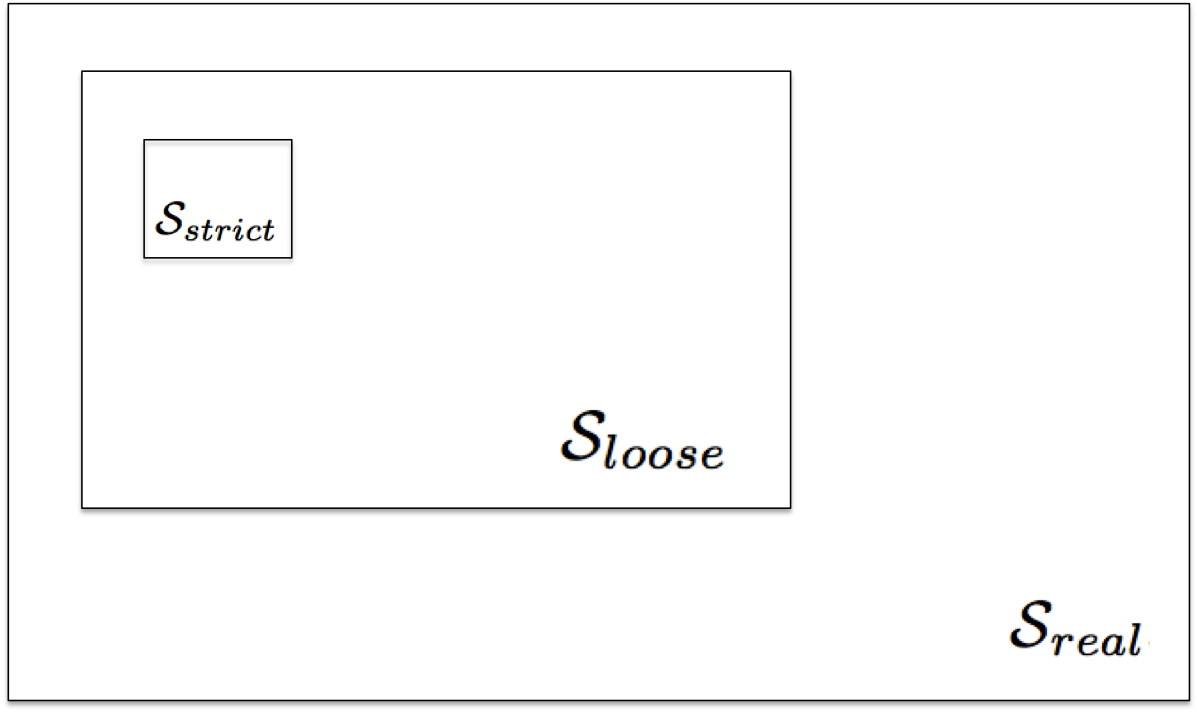
\includegraphics[width=0.7\columnwidth]{Figures/dataset_sizes.png}
	\caption{Representation of our $\mathcal{S}_{strict}$, $\mathcal{S}_{loose}$ and $\mathcal{S}_{real}$ scenarios.}
	\label{fig:scenarios}
\end{figure}

To understand the impacts of temporal consistent learning, we perform a comparative analysis of the three above scenarios under two distinct environments:

\begin{itemize}
	\item \textit{laboratory conditions} where traditional cross-validation methodologies can be applied;
	\item \emph{real-world conditions} where time is relevant and we analyze the behavior of the classifier with temporal-based methodologies.
\end{itemize}

This will help us understand if one should take precautions when using classical evaluation methodologies, as these do not take into account time dependency between samples.

We also provide several improvements to the model.
One of these come under the form of a multi-layer approach, which instead of classifying a sample as malware or goodware, also provides information regarding the type of malware.
Our other improvement regards providing more information about a sample to the model, by using dynamic information extract during runtime, in order to obtain higher scores.

%%%%%%%%%%%%%%%%%%%%%%%%%%%%%%%%%%%%%%%%%%%%%%%%%%%%%%%%%%%%%%%%%%%%%%%%
\section{Thesis Outline}
\label{section:outline}

Chapter \ref{chapter:related_work} introduces malware by describing some of its history, followed by different techniques to detect malware. We then describe a practical application of a specific analysis technique, from which we obtained our dataset.
We introduce the notion of machine learning and its applications, followed by related work that specifically uses \gls{ml} to detect malware. 

Chapter \ref{chapter:data_collection} describes our initial approach and methodology to help solve the problem of malware detection using \gls{ml}. We detail the data gathering process and how it was analyzed, followed by the labeling process and dataset creation.

Chapter \ref{chapter:static_features} and \ref{chapter:model_improvements} take the created datasets to build a malware detection model based on both static and dynamic features, as well as how these perform under different validation methodologies.

% Chapter \ref{chapter:practical_applications} describes how our model is practically implemented both as an online malware detection service and how it was inserted into a email server to analyze attachments.

Chapter \ref{chapter:conclusions} provides some final remarks on our work, how our model is practically implemented, contributions and possible ideas that may improve the presented work.
 % file "Thesis_Introduction.tex"
\cleardoublepage

%%%%%%%%%%%%%%%%%%%%%%%%%%%%%%%%%%%%%%%%%%%%%%%%%%%%%%%%%%%%%%%%%%%%%%%%
%                                                                      %
%     File: Thesis_Background.tex                                      %
%     Tex Master: Thesis.tex                                           %
%                                                                      %
%     Author: João C. Godinho                                          %
%     Last modified : Apr 2018                                         %
%                                                                      %
%%%%%%%%%%%%%%%%%%%%%%%%%%%%%%%%%%%%%%%%%%%%%%%%%%%%%%%%%%%%%%%%%%%%%%%%

\chapter{Related Work}
\label{chapter:related_work}

The following chapter will go over prior work that closely relates to the topic of our research and areas of contribution.
We approach the definition of malware and how it can be hard to detect and label by providing some background on the subject.
We then proceed to elucidate on different malware detection techniques, from simple methods to more complex approaches, focusing on a specific malware analysis technique that provided the basis for our work.

We advance to the general topic of \gls{ml}, after which we describe related work that studies the use of \gls{ml} in malware detection.
Lastly, we reference prior work that not only tackles our same goal, but also takes into account the impact of \textit{laboratory} \textit{vs.} \textit{real world} scenarios, as well as the notion of temporal based detection, or concept drift.

%%%%%%%%%%%%%%%%%%%%%%%%%%%%%%%%%%%%%%%%%%%%%%%%%%%%%%%%%%%%%%%%%%%%%%%%
\section{Background}
\label{section:background}

The term malware was first used by Yisrael Radai in 1990~\cite{elisan:malware}, before then malicious software was referred to as computer viruses, a notion which was first formalized by Cohen in 1983~\cite{cohen:virus}.
Given term computer virus predates the term malware, it is not uncommon to see both terms used interchangeably.
% For the purpose of this work the term malware is adopted, for reasons explained in the following paragraphs.

To the exponential growth of malware~\cite{av-test:report}, the ability to distinguish between malware samples is crucial.
In the biological world, different types of infections reckon distinctive disinfections, the same applies to the digital world.
The infection method, behavior and subsequently purpose of malware samples vary, hence being able to make a distinction facilitates prevention and disinfection by anti-virus solutions.

There exists no ground truth when it comes to distinguishing malware, leading to subtle differences on the classification and naming of the same malware instance by different parties.
To facilitate the reader's understanding of the topic, the current work will focus on defining malware types based on their propagation and purpose.

With respect to the propagation method, malware can be split into three classes~\cite{kolter:learning}:

\paragraph{Virus.}%\footnote{This work uses virus as a subset of malicious code, hence the choice of using the term malware over virus.}
This type of malware inherits its name from resembling to biological viruses.
A virus is usually composed by two main subroutines.
The first subroutine is responsible for infecting other programs by attaching the virus code, while the second subroutine is the actual malware payload that contains the malware purpose (\ie\ virus payload)~\cite{chen:evolution}.
Viruses are attached to programs and propagate when an infected program is run, either consciously (\eg\ clicking on executables) or unconsciously (\eg\ auto-run features), hence depending on other programs (as hosts) and user interaction.
For viruses to infect new systems, an infected file must be carried between them by a user (\eg\ USB pen, email attachment), reinforcing the user's role in this propagation method.

\paragraph{Worm.} The increasing number of network connected devices facilitates the application of worms to propagate malware.
A worm shares the self-replicating ability of viruses, but discards user interaction and the need for a host.
This is possible by making a worm an independent program that exploits networks to find vulnerable systems to infect with a copy of themselves~\cite{chen:evolution}.
Similarly to viruses, worms can contain additional payload to perform malicious actions on infected systems (\eg\ Blaster worm exploited a vulnerability in RPC for propagation while its payload flooded a Microsoft domain\footnote{W32/Blaster worm, CERT, August 11, 2003 [http://www.cert.org/historical/advisories/CA-2003-20.cfm]}).

\paragraph{Trojan.} While viruses and worms focus on self-propagation, trojans focus on deceiving users into executing them, disregarding propagation.
Trojans try to appeal users with some useful functionality as to allure into running the program~\cite{szor:art}.
By hoaxing users into running them, trojans bypass the need for a host (in the virus case) or an exploit (in the worm case) to perform malicious actions.

\medskip

These three classes are not exclusive and can be used in conjunction to facilitate propagation (\eg\ a virus that relies on a trojan to start propagating).
Given the inexistent standards for malware naming, some literature~\cite{szor:art} define worms as a subset of viruses, as some worms start by attaching to files.
With the general infection methods layered out, the following will succinctly describe the general naming when referring to the malware purpose (\ie\ its payload).

Given the high numbers of malware multiple purposes imply multiple names, as such the following lists some of the most commonly heard names and definitions as given by McAfee~\cite{mcafee:glossary}:

\begin{itemize}
	\item \textit{Adware}: Program that automatically displays advertisement to the user. Most do not cause direct harm.
	\item \textit{Backdoor}: Installs or takes advantage of an unknown entry point to a user's system, allowing remote control of a system.
	\item \textit{Bot}: Short for \say{robot}; A program that receives commands from a cybercriminal and executes them blindly, due to this characteristic, compromised computers are called zombies.
	\item \textit{Dropper}: Program that facilitates the introduction of other malware instances into a system.
	\item \textit{Keylogger}: Program that monitors a user's input (\eg\ keyboard strokes) to steal private information.
	\item \textit{Password Stealer (PWS)}: Program that specifically targets a user's personal information, like usernames and passwords.
	\item \textit{Ransomware}: Program that restricts access to a system/files (usually by encryption) and demands a ransom to allow a user his access.
	\item \textit{Remote Administration Tool - RAT}: Program designed to give an administrator remote control of a system. Similar to \textit{Backdoor} and \textit{Bot}, but usually has higher privileges on infected systems.
	\item \textit{Rootkit}: Program designed to hide the existence of other (malicious) programs, hindering detection of malicious applications.
	\item \textit{Scareware}: Program that fakes the existence of malware and tricks the user into paying for disinfection or into downloading real malware.
	\item \textit{Spyware}: Program that spies on a user's activity through multiple vectors (\eg\ taking prints of a user's desktop/webcam).
\end{itemize}

The ability to name a malware given its propagation method and purpose facilitates detection and disinfection, but given the high quantities of malware, being able to particularly discriminate an instance is helpful.
To that purpose, attempts have been made to create naming conventions for malware.

One of the first attempts was made in 1991, by the \gls{caro}~\cite{caro:naming}.
This attempt was aimed at viruses only and focused on discriminating and relating virus samples.
The convention defines an hierarchical naming with three levels.
The base of the hierarchy is the family name, where structurally similar virus should be grouped.
To further distinguish instances, a group name and major variant name is applied.
To differentiate versions of the same instance and provide additional information about a sample, minor variant name and modifier fields are to be used.
In sum, a virus name should look as following:

\begin{center}\texttt{family.group.major.minor:modifier}\end{center}

To enable differentiation from other types of malware, an improvement to \gls{caro}'s naming was proposed in 1999 by Geral Scheidl~\cite{scheidl:naming}.
Scheidl's proposal included a prefix that consisted of the platform targeted by the malware and a type (\ie\ previously defined classes and names), rendering a more in-depth name:

\begin{center}\texttt{platform.type/family.group.major.minor:modifier}\end{center}

In the Virus Bulletin magazine of January 2002~\cite{virus_bulletin} the naming problem is again addressed, referencing that only a small number of vendors apply \gls{caro}'s names and that the lack of cooperation between anti-virus vendors lead to multiple aliases for malware names.
Again a naming convention is proposed with focus on detail by using three levels of information: malware name, classification and full text description.

Given that no naming convention is widely adopted, anti-virus vendors make use of their own naming that although similar, vary slightly.
This variation raises the redundancy for instances of the same malware as shown by an article published by Symantec in 2002\footnote{A Virus by Any Other Name: Virus Naming Pratices, Costin Riau, June 2, 2002 [https://www.symantec.com/connect/articles/virus-any-other-name-virus-naming-practices]}, stating that the same malware instance has an average of four different names.

The naming problem, although not directly related to the current work, must be taken into consideration as to not influence the classification results.

%%%%%%%%%%%%%%%%%%%%%%%%%%%%%%%%%%%%%%%%%%%%%%%%%%%%%%%%%%%%%%%%%%%%%%%%
\section{Malware Detection}
\label{section:mal_detec}

This section will provide a deeper description of detection methods, from the simplest techniques to more complex ones. The following is based on the work by Peter Szor, \textit{The Art of Computer Virus Research and Defense}~\cite{szor:art}, which although not recent, provides a solid background on detection methods.

To detect malware instances, anti-virus applications are used.
These can also be called scanners, as early detection methods simply scanned for byte sequences to detect malware.
Before going into details on the different detection techniques, it is worth mentioning that scanners can be used as \textit{on-demand} or \textit{on-access} scanners.
On-demand anti-virus are executed only at the user's request.
On-access anti-virus are memory-resident, meaning they load as an application and intercept actions related to file and disk access.
This makes it so that when files are opened, created or closed, the anti-virus scans the changed object.

%%%%%%%%%%%%%%%%%%%%%%%%%%%%%%%%%%%%%%%%%%%%%%%%%%%%%%%%%%%%%%%%%%%%%%%%
\subsubsection{First-Generation Scanners}
\label{subsection:first_gen_scanners}

These type of scanners work at a fairly simple level and focus searching for known byte sequences (\ie\ known to be malware sequences).
The applied principles include:

\paragraph{String Scanning.} A sequence of bytes that is common in a malicious program but not in a regular program is matched against a suspicious file. 

\paragraph{Wildcards.} This method is similar to string scanning, but instead of searching for a fixed sequence of bytes, a more flexible matching is made, allowing to skip bytes or byte ranges.
The method can also include the use of regular expressions for matching.

\paragraph{Mismatches.} Also similar to string scanning, yet there can be $N$ number of bytes in the string that can take any value and in any position (\eg\ the string \say{\texttt{01 02}} with mistmatch of 1 matches \say{\texttt{01 AA}} and \say{\texttt{AA 02}}).

\paragraph{Generic Detection.} This method typically applies both wildcards and mismatches to create generic strings that can scan for several variants of a family of malware, hence being more robust to subtle changes in malware.

\medskip

These principles can be assigned to the signature-based type of methods, as they depend on searching some previously defined byte sequence to be effective.
Their effectiveness depends on an updated knowledge base with the strings to be matched.

Alongside these basic principles, the following can be used in conjunction to improve the scanning speed and reliability:

\paragraph{Hashing.} This term is not a method by itself, but techniques that speed up searching algorithms, enhancing previous methods.
It takes advantage of the hash table data structure to match malware signatures.

\paragraph{Bookmarks.} This method is both used to provide more accurate detections and disinfections. Bookmarks provide specific locations for where strings are to be searched (\ie\ offsets).

\paragraph{Top-and-Tail Scanning.} Like hashing, this principle is used to speed up detection by scanning the start and end of a file, instead of the entire file.
The technique is mainly effective when dealing with viruses that prefix or append data to files.

\paragraph{Entry-Point and Fixed-Point Scanning.} This technique also improves the speed of anti-virus scanners.
By taking advantage of the structure of binary objects this method can start scanning at the entry-point of an object, or alternatively use the entry-point plus some fixed size as a fixed-point from where to start scanning.

\paragraph{Hyperfast Disk Access.} This last technique also provides a speed improvement.
It does so by bypassing operating system level \gls{api} to read the disk directly with the \gls{bios}.
In addition to improve the scanners performance, this principle is also useful as an anti-stealth technique, given it works below the filesystem layer.
It is worth noting that this technique is hard to implement nowadays due to the high variety of file systems and disk controllers.

%%%%%%%%%%%%%%%%%%%%%%%%%%%%%%%%%%%%%%%%%%%%%%%%%%%%%%%%%%%%%%%%%%%%%%%%
\subsubsection{Second-Generation Scanners}
\label{subsection:second_gen_scanners}

These methods improve on the previous generation by doing an analysis at a higher level of abstraction.
Where first-generation scanners would match sequences of bytes, second-generation scanners also look at the bytes representation.
The applied principles include:

\paragraph{Smart Scanning.} This method takes the assembly representation of the bytes into account and instructions that have no effect (\eg\ \texttt{NOP}) can be skipped.
The resulting signature is smaller and more easily detects mutations.
The same principle can be applied to textual malware (\eg\ scripts), where extra white spaces have no effect.

\paragraph{Skeleton Detection.} This method is specifically useful in detecting textual malware (\eg\ macros) families.
By parsing the macro statements line by line, the scanner can drop nonessential statements.
The result can be seen as a skeleton of the full macro that contains only the relevant code that appears in malware.

\paragraph{Nearly Exact Identification.} This method provides a more accurate way to detect malware.
First-generation scanners base detection mainly on a byte sequence, whereas nearly exact identification makes use of double-string detection.
The principle comes from using two strings to match a given malware, if only one of those strings match, then it is likely to be a variant of a known malware.
This is specifically useful to identify same family malware.
Another nearly exact identification method applies a checksum to a range from the malware body, this has the added benefit of better accuracy without overloading the anti-virus database.

\paragraph{Exact Identification.} This method enhances the previous method by adding the ability to differentiate malware variants.
It does so by using as many checksum ranges as needed to identify variants of the same malware, improving the accuracy and facilitating disinfection.

\medskip

Like in the previous generation, these methods fit into signature-based, hence still being highly dependent on an updated knowledge base.

%%%%%%%%%%%%%%%%%%%%%%%%%%%%%%%%%%%%%%%%%%%%%%%%%%%%%%%%%%%%%%%%%%%%%%%%
\subsubsection{Algorithmic Scanning Methods}
\label{subsection:algorithmic_scanning}

These methods are not so focused on direct matching of signatures, but on the routines implemented in the scanner that allow the detection of malware.
Early implementations of algorithmic scanning were hard-coded in the anti-virus, but with different types and families emerging, the hard-coded algorithms could easily become obsolete.
To overcome this, vendors would introduce more specific routines for malicious programs when updating the anti-virus.

Examples of these methods are filtering, where signatures are only applied if an object meets a particular filter; static decryptor, which detects encrypted malware; and X-ray, which tries to decrypt malware that use simple encryption methods (e.g. \say{\texttt{XOR}} with constant key).

Algorithmic scanning methods are more related to heuristic-based methods, since the focus is developing rules to facilitate malware detection and removal.
These methods also allow for vendors to push new detection algorithms to clients without having to update the entire anti-virus.

%%%%%%%%%%%%%%%%%%%%%%%%%%%%%%%%%%%%%%%%%%%%%%%%%%%%%%%%%%%%%%%%%%%%%%%%
\subsubsection{Code Emulation}
\label{subsection:code_emulation}

This detection technique uses dynamic analysis (\ie\ analysis during runtime) to detect malware by simulating code execution.
A virtual machine is used to simulate the system's components, thus the malicious files are encapsulated and no code is executed by the real processor.

Code emulation can be faster than using algorithmic scanning methods when dealing with encrypted/obfuscated malware, as the code can be emulated and the decrypted/deobfuscated code is much easier to obtain.
The downside to emulation comes from a time perspective, as more resources are needed to emulate code.

%%%%%%%%%%%%%%%%%%%%%%%%%%%%%%%%%%%%%%%%%%%%%%%%%%%%%%%%%%%%%%%%%%%%%%%%
\subsubsection{Heuristic Analysis}
\label{subsection:heuristic_analysis}

This detection technique takes into account several characteristics of malicious software, both static and dynamic.
Examples of such characteristics are code execution starting in uncommon sections, suspicious code redirection or incorrect size of code in header.

Using the previously described methods, heuristic analysis can take into account different characteristics that are present or absent to assert if a file is deemed malicious or not.

The upside of this technique is that it allows for never seen malware to be correctly flagged, but brings the downside of a higher amount of false positives.

%%%%%%%%%%%%%%%%%%%%%%%%%%%%%%%%%%%%%%%%%%%%%%%%%%%%%%%%%%%%%%%%%%%%%%%%
\subsubsection{Sand-Boxing}
\label{subsection:sand_boxing}

This detection technique builds on the already mentioned code emulation, but with a higher level of complexity.
With sand-boxing the whole system is emulated (\ie\ virtualized) and suspicious or malicious programs have access to a copy of the real resources, effectively limiting the effects of the program and consequently protecting the system.

This technique allows to extract dynamic information without compromising the real system, which can then be used to detect if a suspicious program is malware, by applying the aforementioned techniques, and to help analyze new types of malware.
This technique demands more resources then previous ones and may not be ideal to use inside an anti-virus application.

Other downsides of sand-boxing come as compatibility issues, the possibility of malware detecting virtualization, which can hinder analysis, or even if the virtualization software is vulnerable and malicious code can escape the sandbox into the host machine.

\medskip

Detecting malware is not as simple as applying one of the mentioned techniques, different methods work best in different scenarios, hence anti-virus need to balance the usage of these techniques to keep systems protected.

%%%%%%%%%%%%%%%%%%%%%%%%%%%%%%%%%%%%%%%%%%%%%%%%%%%%%%%%%%%%%%%%%%%%%%%%
\section{Cuckoo Sandbox and Malwr}
\label{section:cuckoo}

Building on the last described method of sand-boxing, this section will describe a specific implementation of sand-boxing, namely Cuckoo.
Cuckoo Sandbox is a malware analysis system created by Claudio Guarnieri~\cite{tool:cuckoo}.

When analyzing a malware sample, an analyst will have to create his own virtual environment, transfer the sample into that environment and manually interact with the sample to see how it behaves and what it does.
Cuckoo facilitates analysis by automating this process.

The Cuckoo system will take the sample to analyze and run it inside a predefined virtual environment (\eg\ Windows XP).
The system is then capable of simulating user interaction, take screenshots of the environment, extract static and dynamic information about a sample, monitor network traffic and perform memory analysis.
The time spent doing the analysis can be configured by the user.
Upon finishing the analysis the system provides reports about the sample. The reports' information can be divided into 5 sections:
\begin{itemize}
	\item \textbf{Quick Overview} which includes information like: file type and details; analysis duration; signatures (\ie\ predefined patterns Cuckoo deems suspicious); screenshots during runtime; hosts and domains contacted; files, mutexes and registries used.
	\item \textbf{Static Analysis} which includes information like: file version information; file sections; resources (\eg\ icons); statically imported libraries and their functions; output of the \texttt{strings}\footnote{Linux binary that outputs the strings of printable characters in files.} command on the file; VirusTotal~\cite{tool:virustotal} classification report.
	\item \textbf{Behavioral Analysis} which includes information like: spawned processes; \gls{api} call order for each process.
	\item \textbf{Network Analysis} which includes information like: domains and their resolved IPs; HTTP requests; IRC traffic; SMTP traffic.
	\item \textbf{Dropped Files} which includes information about files created by the sample: their size, name and hash.
\end{itemize}

Some of the defined sections are not always available.
Their availability depends both on a successful analysis by Cuckoo, as well as the type of submitted file.
For example, only binary executables (\eg\ \gls{dll}, \gls{pe}) provide static analysis information.

The creator of Cuckoo and one of its developers, Alessandro Tanasi, also created a free malware analysis service, Malwr~\cite{tool:malwr}.
This service implements the Cuckoo system and allows users to upload their own files, which are then run with Cuckoo.
The service is presented as a web application that takes in samples and returns a report with Cuckoo's results.
An example of the behavioral analysis (\ie\ created process and \gls{api} calls) can be seen in Figure \ref{fig:malwr_sample}.

\begin{figure}[!htb]
	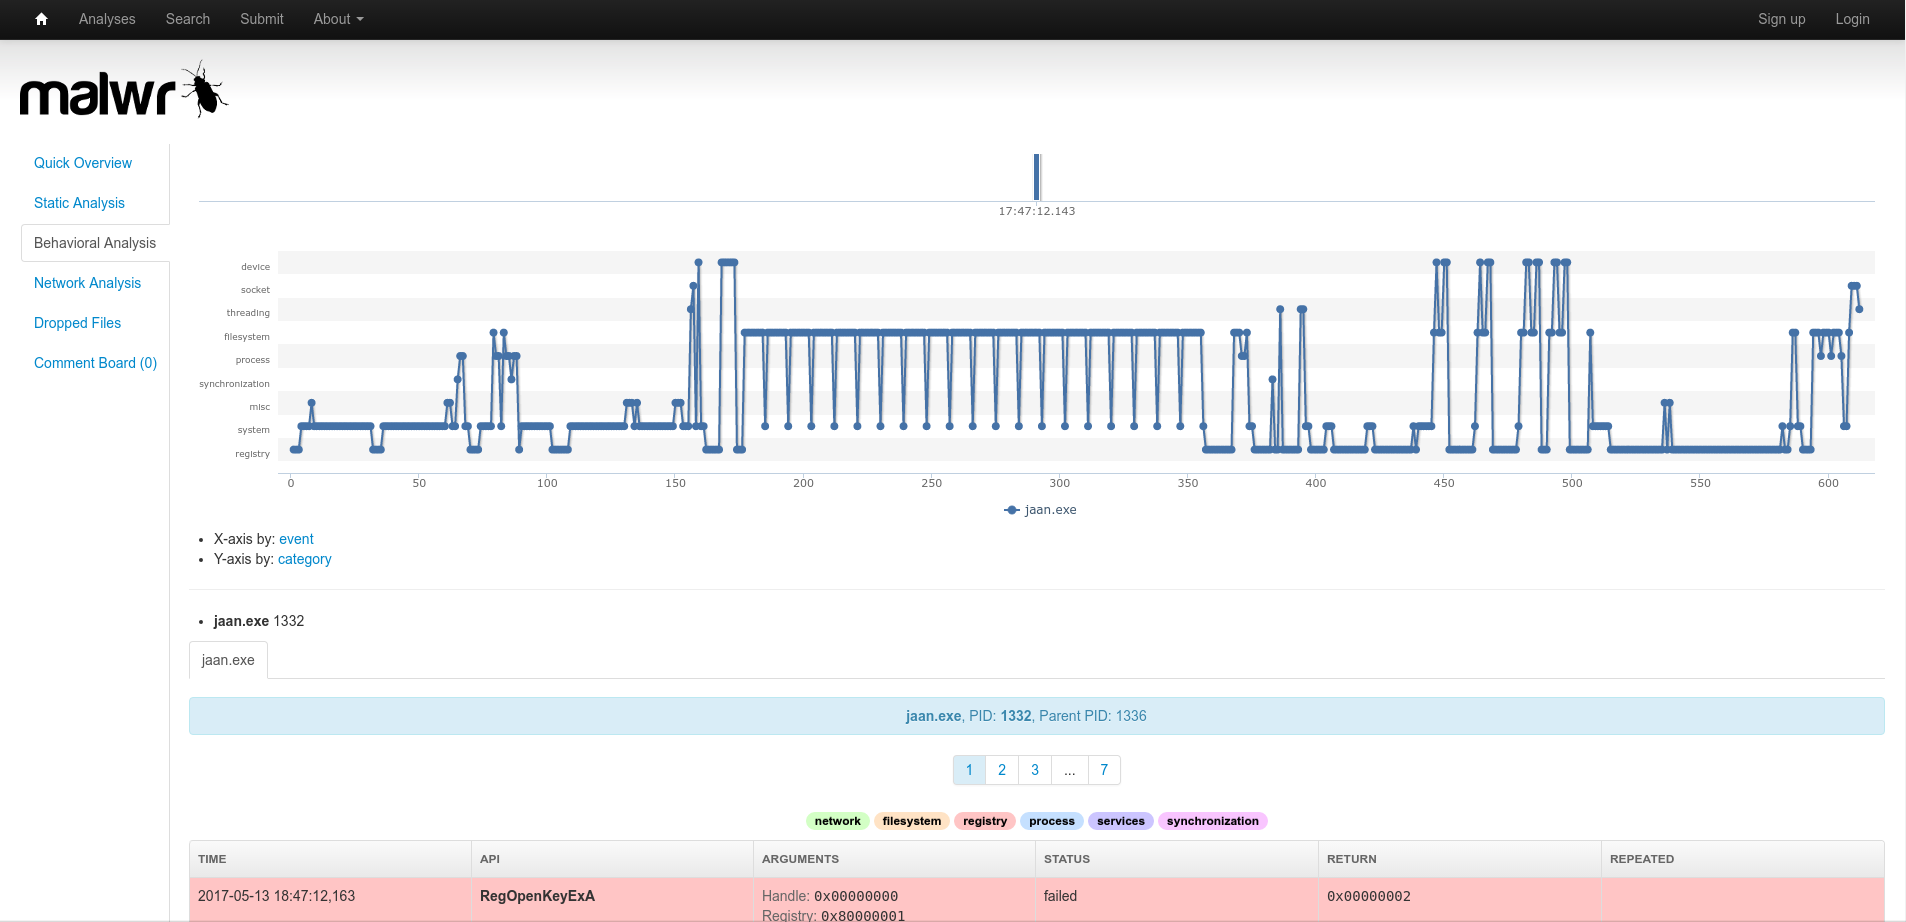
\includegraphics[width=\columnwidth]{Figures/malwr_sample.png}
	\caption{Example of a behavioral report from Malwr.}
	\label{fig:malwr_sample}
\end{figure}

Unfortunately at the time of writing, Malwr is under maintenance hence the provided image will be outdated once the new version is live.

For the purpose of detecting malware via \gls{ml}, the reports provided in Malwr supply various information that can be used for the current work.
The whole website content is provided under \gls{cc} CC-BY-NC-SA 3.0\cite{cc-by-nc-sa} license, allowing use of the data for this work's purpose, as long as credits are maintained.

%%%%%%%%%%%%%%%%%%%%%%%%%%%%%%%%%%%%%%%%%%%%%%%%%%%%%%%%%%%%%%%%%%%%%%%%
\section{Machine Learning}
\label{section:ml}

Even before the modern concept of computer proposed by Alan Turing, mankind has always searched for ways to either automate or facilitate more complex tasks.
With the technological advances that provide higher computation power, computer science fields like \gls{ai} have greatly improved in recent years.

One of the \gls{ai} fields that has benefit from the technological advances is \gls{ml}.
The current subsection will provide a more detailed description of \gls{ml} and its use for the current work.

\gls{ml} is a subset of \gls{ai} in which algorithms are applied to learn and make predictions on data, or more formally defined by Tom Mitchell~\cite{mitchell:ml}:
\begin{center}
\say{\emph{A computer program is said to learn from experience $E$ with respect to some class of tasks $T$ and performance measure $P$, if its performance at tasks in $T$, as measured by $P$, improves with experience $E$.}}
\end{center}

A noteworthy nuance about the given definition, and the \gls{ml} field in general, is that these algorithms are not designed to deal with specific problems.
Meaning that as long as a learning problem is well defined through $T$, $P$ and $E$, an algorithm based on these three features is able to learn, but not necessarily solve any problem.
This creates a contrast to \gls{ai} fields, where algorithms are built for specific tasks.

After defining a learning problem, to obtain a useful outcome (\ie\ model) one or more learning algorithms are applied.
Learning algorithms fall within one of the following classes: \textit{supervised learning}; \textit{unsupervised learning}; \textit{semi-supervised learning} or \textit{reinforcement learning}.

Each of the categories is defined on how the problem is learned . A more detailed description, as seen in \cite{norvig:ai} is as follows:

\paragraph{Supervised Learning.} In this category the program is given a corpus (\ie\ experience) with input-output pairs and it must learn how to map a never seen input into the correct output.
Within supervised learning, a learning problem can be further classified into a classification problem, if the output is a set of finite values (\eg\ is it going to rain tomorrow?), or into a regression problem, if the output is continuous (\eg\ how likely is it to rain tomorrow?).

\paragraph{Unsupervised Learning.} In this category the program is given a corpus and it must learn patterns from the input, hence no correct or wrong output is expected, only how different input relates.
The most common task in unsupervised learning is clustering, where input is grouped based on similar characteristics.

\paragraph{Semi-supervised Learning.} This category is a combination of the previous ones and exists because sometimes the learning problem is based on a dataset that combines both labeled and unlabeled inputs or on a dataset that contains noisy data. 
The combination of supervised and unsupervised learning provides a better overall result in such scenarios.

\paragraph{Reinforcement Learning.} In this category the program is given a problem through a set of states and a set of actions it can perform.
At any given state the program performs an action which results in a reward or punishment.
The cumulative reinforcement at each state teaches the program the best and worse actions for each state.

\medskip

The current work will fit into the supervised learning category, with the purpose of creating a model to assert whether a given sample is malware or not.
This problem can be seen as whether a pure classification problem, with a binary output, or as a regression problem, with the likelihood of a sample being malware.

\medskip

When designing a learning system, multiple choices must be taken into consideration.
A brief description of what should be taken into account is given as seen in~\cite{mitchell:ml}:

\begin{itemize}
	\item \textbf{Training experience} is the first choice, as it can have a significant impact on the success or failure of the learner.
	The feedback provided by the experience can be direct or indirect, affecting the end result of the system.
	Another important aspect is how the experience represents the distribution over which the performance is measured, meaning how well the experience represents the environment where the system is to be used.
	Being what is going to be fed to the learner (\ie\ features), it must be well thought out and understood.
	\item \textbf{Target function} is the next choice, representing what is to be learned.
	The function takes as input the set of features that represent the problem and (ideally) outputs a solution to the task.
	\item \textbf{Target function representation} is the remaining choice, this is where a learning model is applied to learn the given task.
	The choice is of great importance, given it will influence how well the system performs under evaluation.
\end{itemize}

Given the nature of the purposed work as a classification problem, many models can be applied as a representation for the target function.
The following describe some models taken into consideration during implementation.

\paragraph{Decision Tree Learning.~\cite{mitchell:ml}} These methods are used to approximate discrete-valued target functions, where the learned function is represented as a decision tree.
The decision tree is built based on how much information each attribute gives (\ie\ information gain).
These are best suited for problems where instances are represented by attribute-value pairs of discrete values and problems where data may contain errors.
The shortcomings with decision tree methods include how deep to grow the decision tree, how to handle continuous attributes and handling attributes with different weights.

\paragraph{\gls{ann}.~\cite{mitchell:ml}} These methods can be used for real-valued, discrete-valued and vector-valued target functions.
\gls{ann}'s are inspired in part by neurons in the biological world, hence being represented as directed graphs.
\gls{ann}'s can be applied to the same type of problems as decision trees, but these can also handle instances represented by many attribute-value pairs.
\gls{ann}'s have the downsides of being time consuming to train and to easily overfit the training data (\ie\ training data is learned well, but fail to generalize to new data).

\paragraph{Bayesian Learning.~\cite{mitchell:ml}} These methods use a probabilistic approach to inference.
The reasoning is that the optimal decision can be related to some probabilistic distribution of the data.
Bayesian learning proves to be effective for text classification tasks and also provides useful insight on other learning algorithms that do not deal with probabilities.
The shortcomings can be related to the need of requiring initial knowledge, as well as computational cost to achieve the best hypothesis, which grows with the number of hypothesis.

\medskip

Even though the field of \gls{ml} is broad, the main focus is always the ability to generalize a given task.
For every learning task multiple models can be applied, which complicates the task of choosing a model.

Although being able to try different models and how they compare to each other benefits the end result, this work focused solely on a single model, reasoned in Section \ref{section:model_selection_evaluation}.
Doing so enabled to us to spend more time understanding the impacts of \textit{ground-truth} and temporal consistency.

%%%%%%%%%%%%%%%%%%%%%%%%%%%%%%%%%%%%%%%%%%%%%%%%%%%%%%%%%%%%%%%%%%%%%%%%
\section{Machine Learning in Malware Detection}
\label{section:ml_md}

The previous Sections gave a general understanding on how anti-virus software detects malware and how the \gls{ml} field can be applied to learn tasks without having to define specific algorithms.
This section will describe research that aggregates both malware detection and machine learning.
Authors make use of specific \gls{ml} classifiers like Naive Bayes (NB), \gls{lr} and \gls{svm} to design systems that learn to detect malware.

The main focus is to note the choices made by the authors relative to the datasets, classifiers and their evaluation, all of which were taken into consideration in the current work.

Before analyzing the work done with \gls{ml} in malware detection, it is worth noting how such work is to be conducted.

Rossow et al.~\cite{rossow:practices} present some guidelines for designing malware experiments.
Their work surveys 36 academic publications from 2006 to 2011 that rely on malware execution.
The authors note frequent shortcomings in the surveyed publications regarding assumptions on the use of execution-driven datasets, absence of security precautions taken during experiments and insufficient description of the experimental setup.
The provided guidelines are split into four groups: correct datasets, transparency, realism and safety.

Regarding correct datasets, the publication guidelines include whether goodware samples are to be present in datasets, how the dataset is balanced over malware families and if training and evaluation datasets should have different families.
The authors note that at least nine distinct papers suffer from significant problems relating to the correctness criteria.

With regards to transparency, the given guidelines include the interpretation of false positives, false negatives and true positives, family names of employed malware samples and how they were named.
In the surveyed papers, it is noted that the majority do not interpret the numeric results and a fifth do not name the malware families contained in the datasets.

Regarding realism, the paper introduces guidelines which include relevance and variety of malware families and real-world evaluations.
The authors note that only a minority of papers include real-world evaluations and very few offer significant sample sizes, making it difficult to judge practical use of the methodology.

With regards to safety, the given guidelines focus on containment policies when analyzing malware samples.
The authors note that most papers did not deploy or adequately describe containment.

As mentioned in Section \ref{section:cuckoo}, the current work makes use of the reports in Malwr, hence some the guidelines provided in the aforementioned research do not apply, specifically the safety guidelines.
As for the other guidelines, they were taken into consideration when designing the presented learning system.

\medskip 

On the same note of guidelines, Shabtai et al.~\cite{shabtai:survey} provide a survey directed at the application of machine learning classifiers to detect malware from static features.
Their work concerns the design and evaluation of such systems.
The process is divided into two phases: training and testing.

The training phase includes the creation of a feature vector to represent each file and posterior processing of such vectors to generate a classifier.
The testing phase measures the performance of the classifier by employing classical measures like \gls{tpr} (\ie\ detection rate), and \gls{fpr}.

The authors outline that the work in designing learning systems include how the samples are to be represented (\eg\ byte n-grams, portable executable features, strings), methods to select features (\eg\ gain ratio, document frequency) and finally the classification algorithm (\eg\ \gls{ann}, \gls{svm}).

It is noted by the authors that the use of multiple classifiers with different weights (ensembles) is beneficial to the classification task, as different classifiers work better on different features.

Some problems addressed that are of importance for the presented work include the imbalance problem and chronological evaluation.
Having a balanced dataset of malware and goodware might not accurately represent the real world.
For chronological evaluation the question if whether the usage of old samples for training can aid or hinder the classification of new samples.

\medskip

When it comes to malware detection from static features, Schultz et al.~\cite{schultz:data_mining} present a data-mining framework to detect new, unseen malicious executables.
Their work uses a dataset of 4,266 programs, with 3,625 malicious binaries and 1,001 clean programs, labeled by a commercial anti-virus.
The features include \gls{dll}'s used by the binary, list of \gls{dll} function calls, number of different function calls within each \gls{dll}, strings from the binary and byte sequences.

They apply three different models (RIPPER, Naive Bayes and Multi-Naive Bayes) to different features, achieving a detection rate between 52\% and 98\% and a false positive rate between 5\% and 9\%.
It is worth noting how the application of different models to different features provide very distinct detection rates.
Also worth noting is the size and imbalance of the dataset, where only 23\% of samples are benign in a total universe of 4,266 samples.

The authors describe the malware samples were obtained from various FTP sites and that 5\% were trojans, while the remaining 95\% consisted of viruses, with no remarks are made regarding the involved families.
The majority of benign samples were gathered from a fresh installation of Windows 98, which may not represent the average benign sample.

\medskip

Another application of \gls{ml} to malware detection from static features is done by Nissim et al.~\cite{nissim:al_pdf}.
The authors apply active learning (semi-supervised learning that takes user input) to the detection of malicious PDF files based on static features.
They use a dataset of 6,774 PDF files, including 1,629 malicious and 5,145 benign files, where the benign files were mark as such by Kaspersky anti-virus software.

Their framework works by filtering out all known benign and malicious PDF's and passing the remaining files to a \gls{svm} model, which linearly separates files based on an initial training set of malicious and benign files.
The ones deemed informative are flagged for manual inspecting and used in future iterations of the \gls{svm} model training.
The core idea in this work is to focus on detecting new and unseen instances of malware files with the help of human interaction.

The authors only apply an \gls{svm} model and justify its use due to previous work that provided good results in malware detection, the fact that it is hard for attackers to understand how the model separates files, that it is efficient when combined with active learning and the ability to handle large number of features.

They evaluate their framework by creating 10 subsets of 620 files, with the remaining 574 files used as initial training for the \gls{svm} model.
For each subset the \gls{svm} is trained and choses the most informative files, these are manually inspected, labeled and added to the training set.
By incrementally using a bigger training set with files manually labeled, the authors show a growing detection rate from 92\% in the first subset to nearly 97\% with the last subset.
This is accompanied by a false positive rate from 0.6\% to under 0.2\%.
These results show that their framework is capable of detecting new and unseen files without a very large training set, but with the help of manual inspection.

Their approach on creating subsets for evaluation and using more benign files in the sets can more closely relate to a real world scenario, as new malicious content is created every day, but it is still less then the amount of benign content.

The authors fail to describe why the chosen features work, this might be related to the use of an \gls{svm}, which makes it difficult interpret the parameters of the model.

\medskip

With regards to malware detection from dynamic features, Rieck et al.~\cite{rieck:dynamic} propose a framework for automatic analysis of malware behavior using machine learning.
Their approach applies both unsupervised (clustering) and supervised (classification) learning to identify novel malware classes and assign unknown to the discovered classes.
Worth noting is that the mentioned work does not deal with goodware samples, focusing only on identifying different malware families.

Their framework starts by executing and monitoring the malware binaries in a sandbox environment, producing sequential reports that contain the operations and actions performed (system calls and their arguments).
The reports are embedded in a high-dimensional vector space and \gls{ml} techniques for clustering and classification are applied.

To optimize the processing of reports, the authors propose a special representation of behavior, namely \gls{mist}.
This representation encodes the monitored system call and its arguments using short numeric identifiers.
Different levels of specificity can be obtained since the arguments are arranged in blocks.
For variable-length arguments an index number is used, which can be mapped to the original content. Figure \ref{fig:mist} shows the schematic overview of \gls{mist} instructions.

\begin{figure}[!htb]
	\centering
	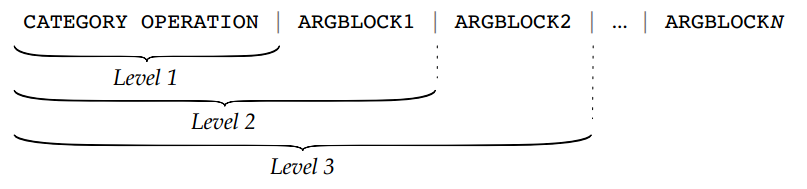
\includegraphics[width=0.7\columnwidth]{Figures/mist.png}
	\caption{\gls{mist} representation as seen in \cite{rieck:dynamic}}
	\label{fig:mist}
\end{figure}

An example of a MIST instruction could be as following:

\begin{center}\texttt{03 05 | 0100000001 | 00006ce5 | 000066fc}\end{center}

This instruction contains four levels.
The first level contains the category and operation, while the remaining levels each contain an argument block.
By variating the level, different granularities can be achieved.

The authors create a vector space for each report that represents the behavior of the sample.
The vector is conceived by creating \textit{Q-grams}.
These are the result of applying a sliding window of size $q$ to the MIST report and constructing a binary vector where every position is whether the report contains the sequence of size $q$ or not.
The size of the vector varies with the number of possible instructions and the size $q$ of the window.

The authors implement their own clustering and classification algorithms for the task at hand.
The evaluation data consists on two sets, a reference set of 3,133 malware reports with 24 different malware families, to be used to evaluate and calibrate the framework, and an application set of 33,698 unknown malware reports taken over a course of seven days.

On the reference set authors apply F-measure for evaluation, which uses precision and recall as parameters, the maximization of F-measure reflects high precision and recall.
The results yield an F-measure over 0.936, which surpasses previous research for both clustering and classification.

On the application dataset authors apply their methodology and achieve 434 clusters (\ie\ malware families).
To the ten largest clusters authors take the most frequent anti-virus label for each cluster using Kaspersky anti-virus.
They note that one anti-virus label is prevalent for each of the ten clusters, assuming that their framework successfully discovers and classifies unknown malware families.

By applying their framework to two different sets, where one was created from real-world samples, the authors show how their framework is applicable to a real-world scenario.

\medskip

Miller et al.~\cite{miller:rev_int} provide a system which relates to \cite{nissim:al_pdf}, as it applies expert reviewers as a limited labeling resource.
Their work uses both static and dynamic features to detect malware and uses manual label together with \gls{ml} to improve the overall result.
The authors evaluate their design on an enormous dataset of 1.1 million binaries spanning 2.5 years, taken from submissions made at VirusTotal, a service similar to Malwr.
Alongside the enormous dataset, the authors also make sure that training data predates evaluation data, contributing to an evaluation with high realism.

With regards to the design of the system, it consists of a detection and a training pipeline.
The detection pipeline takes a binary, extracts the features and applies the current model to classify the binary as malicious or benign.
The training pipeline takes binaries labeled by the manual reviewer, VirusTotal and from the current model, extracts the features and trains the new model.

The system uses multiple static and dynamic features from binaries, including: binary metadata, digital signing, static imports, dynamic imports, file operations, mutex operations, network operations, processes and Windows \gls{api} calls.
The authors chose to use \acrfull{lr} as the classifier, basing their choice on the fact that it predicts a real-valued quantity, which enables the use of a threshold and therefore allows the creation of a tradeoff between true and false positive rates, by adjusting the threshold.
\gls{lr} also assigns a weight to each feature, which allows to comprehend which features are more discriminating.

On evaluation, authors show that when ignoring temporal consistency, results inflate up to 20\% at a 0.5\% false positive rate.
When considering temporal consistency, results range from 65\% to 75\% true positive rate with a false positive rate range from 0.1\% to 1\%.

Another remark made in this article is that vendors prefer false negatives over false positives (\ie\ wrongly classifying malware as goodware over wrongly classifying goodware as malware).
When looking at duplicated samples, 29.6\% of those samples increased in the number of detections as malware and only 0.25\% decreased the number of detections.

\medskip

On the topic of methodologies that resemble real-world conditions, Srndi\'c et al.~\cite{vsrndic2013detection} train and validate their malicious PDF detector under laboratory and real-world conditions.
Laboratory conditions consist on applying regular cross-validation, whereas real-world conditions validate a newer dataset with a model created from outdated data (\ie\ older then the validation), and also validate the model when the validation set spans one week and the training is gathered in the previous 4 weeks.
They show that laboratory conditions inflate the results, when compared to real-world conditions.

Our work enhances these methodologies by analyzing the performance variation when the distance between the training and validation set increases and decreases, as well as analysis on how reducing the size of the training without compromising the results.

\medskip

Kolter et al.~\cite{kolter:learning} learn to detect malicious executables in a dataset with under 4,000 samples, obtained from reliable sources, and evaluate their model under standard cross-validation and by gathering newer malware samples to validate for new and unseen samples.
They show how the model provides optimal results under cross-validation, but for the unseen samples lower scores are obtained.
Our work considers these results to compare how reliability affects performance.

Deo, A. et al.~\cite{deo2016prescience} focus over the problem of \gls{ml} models becoming antiquated over time, given how malware evolves.
This problem is seen as concept drift, where the performance of a model over time diminishes, as the statistical properties of malware (\ie\ features) change over time.
They study how probabilistic predictors can help minimize the aforementioned problem, by indicating when retraining of a given model is necessary. 

Jordaney, R. et al.~\cite{jordaney2017transcend} also study the problem of concept drift in malware classification models, focusing on providing metrics, based on statistical comparison of samples, to detect when should a model be retrained. 

Both \cite{deo2016prescience} and \cite{jordaney2017transcend} are on the subject of our work, regarding the problem of concept drift, but differ on the study-case.
In our work we acknowledge the concept but focus on its relative effects and how one can balance the size of needed training data \textit{vs.}\ validation data, when maintaining a temporal consistent dataset.
Whereas their work provide indicators for when should a model be retrained when the problem of concept drift becomes significant.

\medskip

Perdisci et al.~\cite{perdisci:behavior} use an unsupervised learning approach to cluster malware using malicious network traces.
Although their work does not directly relate to the current work, it also deals with the malware naming problem.
To validate the obtained clusters, the cohesion and separation among clusters is measured in terms of the labels given by anti-virus vendors.

To derive the cohesion and separation, a graph for each cluster is constructed.
Each node is a malware label given by some vendor and an edge connects two nodes if the labels appear together in any malware sample.
Weights are assigned as $1 - \dfrac{m}{n}$, where $m$ is the number of times the different labels appear together and $n$ is the number of samples in the cluster.
From the graphs authors can then measure the cohesion and separation of clusters.

The authors use the aforementioned method to evaluate their results, but the approach can be useful to label and balance malware datasets that contain various anti-virus labels.

\medskip

Regarding the malware naming problem, Sebastián, M. et al.~\cite{sebastian2016avclass} develop \textit{AVClass}, a tool that given a set of antivirus vendors, outputs the most likely family name.
They test their tool under 10 datasets, totaling 8.9 million samples, with results showing an F1 measure up to 93.9\% on labeled datasets.
The tool takes as input the labels as seen in VirusTotal, tokenizes the labels, replaces known aliases and general names (\eg\ win32, trojan, generic), ending with possible family names. These remaining names are counted and the most frequent one is given as family name, Figure \ref{fig:avclass} exemplifies the stated process.

\begin{figure}[!htb]
	\centering
	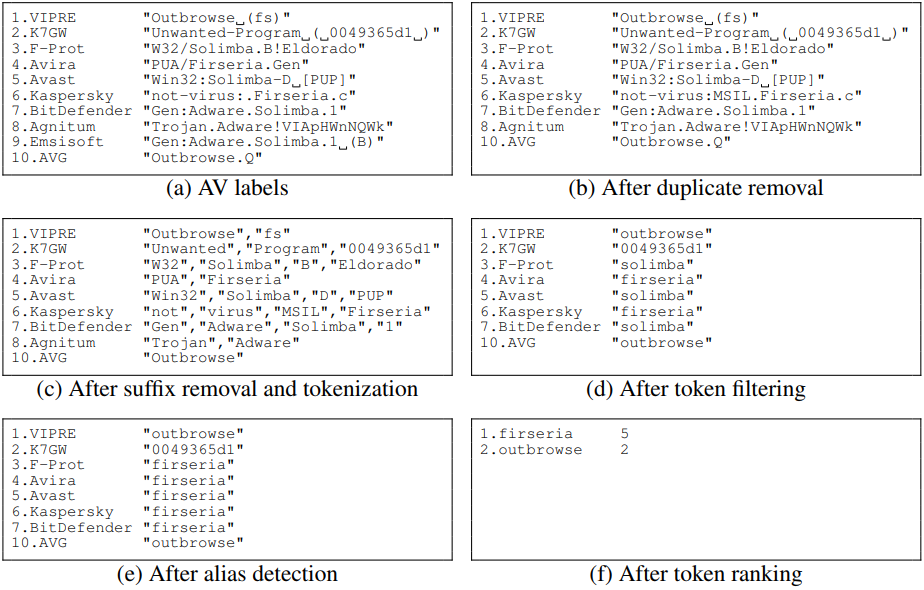
\includegraphics[width=\columnwidth]{Figures/avclass.png}
	\caption{AVClass running example.}
	\label{fig:avclass}
\end{figure}

Our work takes advantage of this tool, not to label malware families, but with minimal modifications, to label more general malware classes (\eg\ trojan, virus).

\medskip

Overall the presented research provides useful insight for the current work. Decisions like the handling of the dataset, how and which features are to be extracted from samples, which and why \gls{ml} classifiers should be used and how and why the evaluation should be made.
 % file "Thesis_Background.tex"
\cleardoublepage

%%%%%%%%%%%%%%%%%%%%%%%%%%%%%%%%%%%%%%%%%%%%%%%%%%%%%%%%%%%%%%%%%%%%%%%%
%                                                                      %
%     File: Thesis_Data_Collection.tex                                 %
%     Tex Master: Thesis.tex                                           %
%                                                                      %
%     Author: João C. Godinho                                          %
%     Last modified :  Apr 2018                                        %
%                                                                      %
%%%%%%%%%%%%%%%%%%%%%%%%%%%%%%%%%%%%%%%%%%%%%%%%%%%%%%%%%%%%%%%%%%%%%%%%

\chapter{Data Collection}
\label{chapter:data_collection}

In the current chapter we detail our initial approach to construct a machine learning model that detects malware based on static and dynamic features.
This first approach was to create a dataset of malware and goodware to feed into a ML model.
We start by describing how the training data was collected, followed by how it was analyzed.
We then proceed to label the samples with help of the aforementioned analysis.

%%%%%%%%%%%%%%%%%%%%%%%%%%%%%%%%%%%%%%%%%%%%%%%%%%%%%%%%%%%%%%%%%%%%%%%%
\section{Data Sources}
\label{section:data_sources}

The purpose of this step is to obtain a corpus from which information
about malware and goodware can be extracted.
To minimize any possible bias towards data collection, and to save the overhead time of collecting and analyzing samples, we chose to take advantage of the publicly available reports from Malwr \cite{tool:malwr} service.
As previously mentioned in Section \ref{section:cuckoo}, Malwr is a free online service that does static and dynamic analysis on submitted files using Cuckoo \cite{tool:cuckoo}, which are then accessible in an HTML report.

To enrich our knowledge about samples' \textit{ground truth} we resorted to two other online repositories: \gls{nsrl} \cite{tool:nsrl} and VirusShare.com \cite{tool:virusshare}, these provide metadata (\eg\ MD5 hash) regarding known goodware and malware samples, respectively.
As \gls{nsrl} contains a collection of digital signatures of known, traceable software applications, if a sample is present in this collection, we are more confident it is indeed goodware.
On the other hand, VirusShare.com is a repository of malware samples, hence a sample present in this repository gives us a higher confidence it is indeed malware.

Our data extraction methodology for Malwr and VirusShare.com was based on applying a common data extraction technique, where online data is saved locally or in a central database for further analysis. This technique, called \textit{scraping}, was done using Scrapy \cite{tool:scrapy}, a Python scraping library.

As for the \gls{nsrl} repository, information was provided in textual format, which led us to use Pandas \cite{tool:pandas}, a Python data analysis library, to extract and analyze the data.


%%%%%%%%%%%%%%%%%%%%%%%%%%%%%%%%%%%%%%%%%%%%%%%%%%%%%%%%%%%%%%%%%%%%%%%%
\section{Data Analysis}
\label{section:data_analysis}

The following provide a detailed analysis of the available data sources, done by using Pandas~\cite{tool:pandas}, a Python Data Analysis Library.

%%%%%%%%%%%%%%%%%%%%%%%%%%%%%%%%%%%%%%%%%%%%%%%%%%%%%%%%%%%%%%%%%%%%%%%%
\subsection{High Level Analysis}
\label{subsection:high_level_analysis}

Our first approach was to scrape the list of analysis in Malwr\footnote{Malwr Analysis list [https://malwr.com/analysis/]}.
It is worth noting this scraping did not provide us the full analysis report, only information regarding the type of submission (\eg\ binary, text, archive), its submission date and the sample MD5 hash.

After our initial scraping to obtain a high level view of the available reports, we observed that Malwr had a total of 642,698 submissions, dated between April 16th, 2013 and October 10th, 2016. As can be seen in Figure \ref{fig:samples_count}, there was an increase in sample submission from 2013 up to all time highs in May, June and July of 2014, followed by possibly a downtime period in August 2014.
The service went back up in September 2014, after which it stabilized around 20,000 submissions per month.

\begin{figure}[!htb]
	\centering
	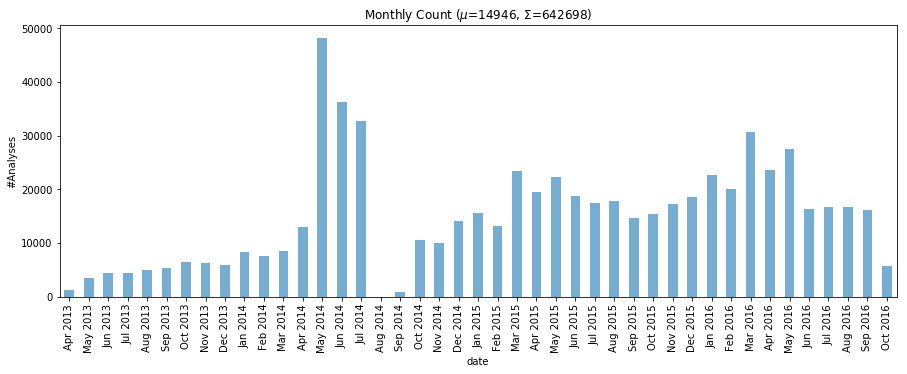
\includegraphics[width=\textwidth]{Figures/samples_count.png}
	\caption[Number of monthly submissions.]{Number of monthly submissions.}
	\label{fig:samples_count}
\end{figure}

Following this initial observation, we measured the percentage of duplicated submissions per month, which vary between 10\% and 20\%, and the percentage of different file types, as shown in Figure \ref{fig:monthly_distributions}.
The file types distribution is interesting, as it shows that executables (\ie\ compiled binary files) took the great majority of submissions up to the end of 2014, after which documents (\eg\ Word, Excel) and text files (\eg\ HTML, JavaScript) started to increase.
As a side observation, this increase might indicate how users are more suspicious of these type of files, given that it is not uncommon to see malware being distributed in documents (under email attachments) and in websites (as JavaScript scripts) in more recent years.

\begin{figure}[!htb]
	\centering
	\begin{subfigmatrix}{2}
		\subfigure[Percentage of duplicated submissions per month (based on MD5).]{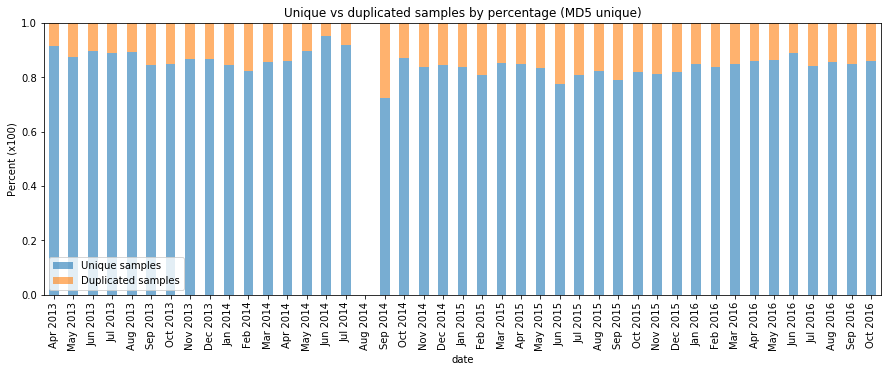
\includegraphics[width=\linewidth]{Figures/samples_dups.png}}
		\subfigure[Distribution of file types per month.]{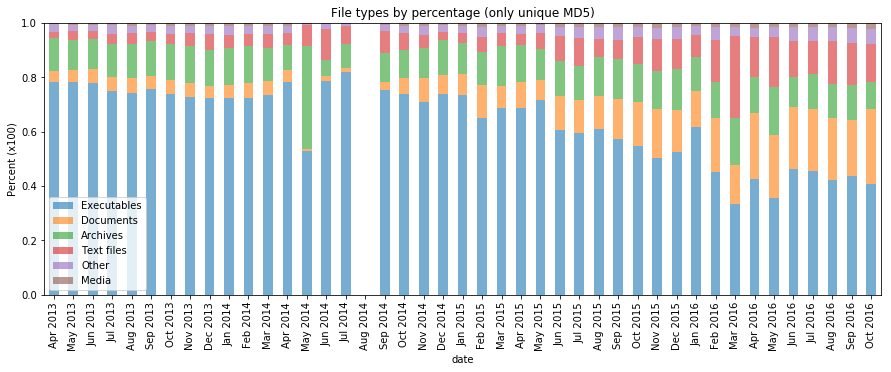
\includegraphics[width=\linewidth]{Figures/samples_types.png}}
	\end{subfigmatrix}
	\caption[Monthly distributions of submissions.]{Monthly distributions of submissions.}
	\label{fig:monthly_distributions}
\end{figure}

Having a better overall understanding on the available reports, and taking into account the limitations of static analysis in \textcolor{red}{Cuckoo} as mentioned in Section \ref{section:cuckoo}, led us to our first data selection criteria: collect reports from \gls{pe} (\eg\ 32bit executables, DLL's) submissions only.
This selection reduces the number of available reports to 388,702 (60.48\% of the total) but enables us to work with more static information.

We went on to extract these reports, again using Scrapy, as HTML files and kept them in a gzip compressed format to save disk space.
A set $\mathcal{R}$ of raw reports, totaling 388,507 submissions was obtained, (different from the
previous amount as some errors could have occurred during scraping) occupying a total of 26GB.

%%%%%%%%%%%%%%%%%%%%%%%%%%%%%%%%%%%%%%%%%%%%%%%%%%%%%%%%%%%%%%%%%%%%%%%%
\subsection{VirusTotal Classifications}
\label{subsection:virustotal_classifications}

As previously mentioned in Section \ref{section:cuckoo}, Malwr aggregates the scan report as provided by VirusTotal (if the sample is already known by VirusTotal), which entails multiple antivirus classifications.
Our next analysis takes advantage of this information to better understand how the samples are labeled and how reliable using the VirusTotal report can be to label our dataset.

After counting the number of different antivirus vendors present in at least one submission, we decided to narrow down to the amount of unique vendors by requiring their presence in at least 95\% of the classified reports.
Doing so guarantees that vendors did not show occasionally and have a strong presence in all classified samples.

By applying this criteria, we narrowed from 97 unique vendors to a smaller set $\VV$ of 38.
This led us to a smaller set $\mathcal{C}\subseteq\mathcal{R}$ of classified reports, which totaled 284,880 submissions. With this new set $\mathcal{C}$ we went on to analyze how reliable the vendors classification is.

Reiterating what was already said, defining and classifying malware is not a trivial task.
The \textit{ground truth} of a sample is hard to obtain, as both antivirus vendors and users disagree on what is malware.
To come to terms with this obstacle, we make use of the classifications given by our set of vendors $\mathcal{V}$ to define a simple malware/goodware criteria: what is the minimum/maximum threshold of positive malware classifications as to label a sample as malware/goodware.

Although this criteria bases itself on a vote policy, adding robustness to the criteria, it also inherits some of the vendors problems: false positives and false negatives. With this in mind, we now aim to understand vendors' accuracy and how they change their classifications.

To study how the classifications vary, we took advantage of the duplicated classified submissions in $\mathcal{C}$. There are 27,798 samples submitted more than once to Malwr, for a total of of 74,916
duplicated submissions $\mathcal{C}_{dups}$ averaging 2.7 submissions per
duplicate.

We now show how we studied the differences between the number of positive classifications on the first and last submission, inspired by Miller's et al. \cite{miller:rev_int} work.

For each duplicated sample in $\mathcal{C}_{dups}$ we counted the number
of positive classifications on the first and last submissions, $\mathcal{P}_f$ and $\mathcal{P}_l$ respectively.
If $\mathcal{P}_f > \mathcal{P}_l$ then we are looking
at a possible false positive (FP), as the number of vendors
classifying the sample as malware decreased.
Conversely, if
$\mathcal{P}_l > \mathcal{P}_f$ we are looking at a potential false negative (FN).
For the case $\mathcal{P}_f = \mathcal{P}_l$ we conclude that vendors are confident regarding their classification for the sample. It is worth noting that there may be cases where $\mathcal{P}_f = \mathcal{P}_l$, but with different vendors (i.e. an equal number of vendors simply switch classification), but given we are looking for a criteria based on a minimum threshold, these cases are not relevant for our analysis.

Figure \ref{fig:dups_frequency} shows the frequency of $\mathcal{P}_l-\mathcal{P}_f$ for each duplicated
sample.
We first note that 44.32\% of duplicated samples change in classification, among which 38.72\% increase its classification (green bars), whereas only 5.61\% decrease (red bars).
There is a clear discrepancy between positive and negative changes, suggesting that vendors favor false negatives (\ie\ increase in positive classifications) over false positives (\ie\ decrease in positive classifications), as also noted by Miller et al. \cite{miller:rev_int}.

\begin{figure}[!htb]
	\centering
	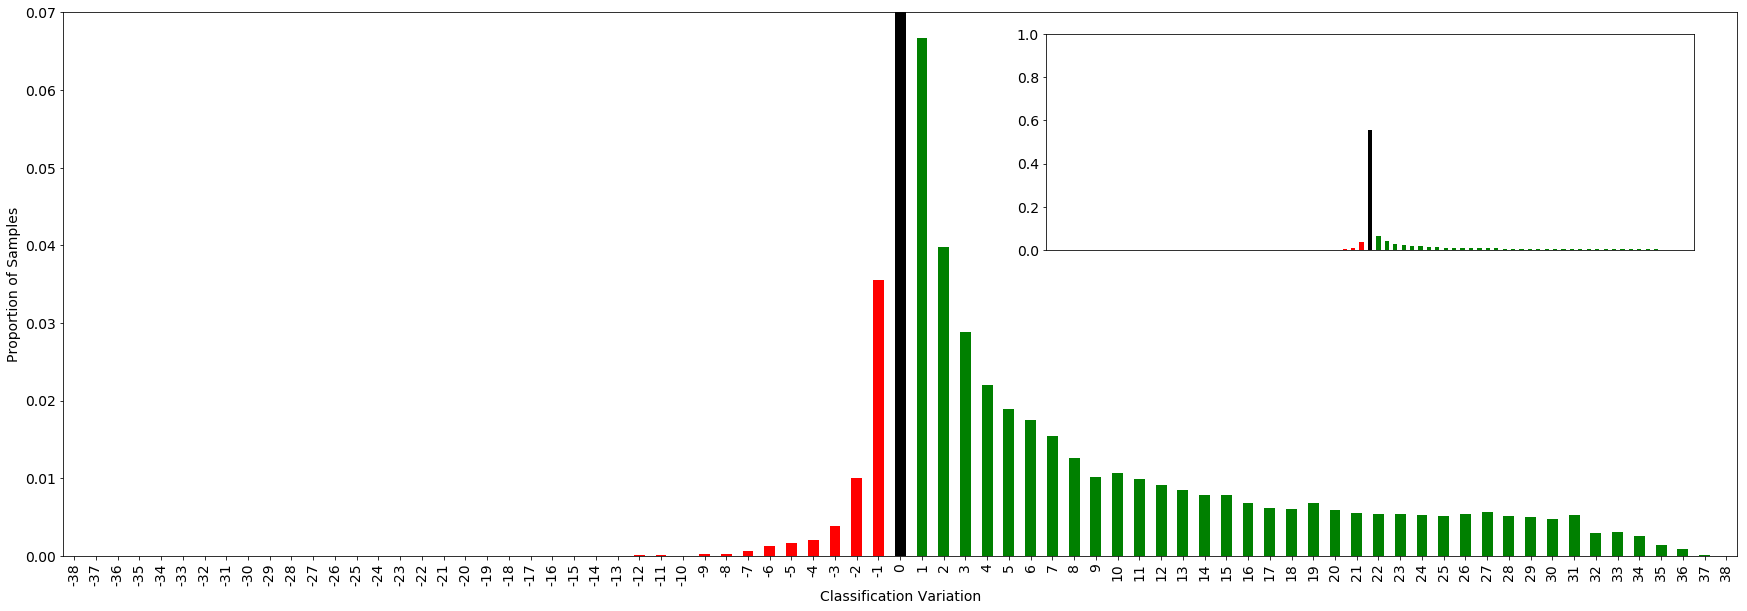
\includegraphics[width=\textwidth]{Figures/dups_frequency.png}
	\caption[Distribution of duplicated samples.]{Distribution of duplicated samples in terms of the changes in the number of
positive classifications between last and first submissions, $\mathcal{P}_l-\mathcal{P}_f$.}
	\label{fig:dups_frequency}
\end{figure}

Another interesting analysis on our samples is understanding the vendors \emph{\gls{dr}} (or True Positive Rate), and \emph{\gls{fpr}}.
Although these formulas are trivially defined respectively as
\begin{eqnarray}
\dr&=&\frac\tp{\#malware}=\frac\tp{\tp+\fn} \\ 
\fpr&=&\frac\fp{\#goodware}=\frac\fp{\tn+\fp}
\end{eqnarray}
we lack ground truth for what is $\#malware$ and $\#goodware$.
To solve this, we must use the available information and propose relative metrics to determine what is positive ($\#malware$) and negative ($\#goodware$).

Our first metric falls back on duplicated submissions again, to define an accuracy metric, $\Madups$. As we have previously shown, 44.32\% of duplicated samples change in classification, which can be translated into vendors acknowledging their own errors.

With that in mind, for each vendor $v\in\VV$, we define a duplicated sample for $v$ (according to $\Madups$) as:
\begin{itemize}
	\item $\tp_v$, \emph{true positive for $v$}, if $v$ classified it positively in both the first and last submissions;
	\item $\tn_v$, \emph{true negative for $v$}, if $v$ classified it negatively in both the first and last submissions;
	\item $\fp_v$, \emph{false positive for $v$}, if $v$ classified it positively in the first submission and negatively in the last submission;
	\item $\fn_v$, \emph{false negative for $v$}, if $v$ classified it negatively in the first submission and positively in the last submission.
\end{itemize}

Figure~\ref{fig:dr_fpr_own} plots each vendors' $\dr_v$ vs.\ $\fpr_v$, under the previously defined metric $\Madups$.
Our first observation is that vendors do acknowledge their own classification errors, as we see a varying $\dr_v$ from 56.82\% to 85.29\%, with a $\fpr_v$ rate ranging from 0.03\% to 6.91\%.
If this was not the case (i.e. vendors would not change their classifications), one would have that $\Pl-\Pf = 0$ for every duplicate and consequently $\dr_v = 1$ and $\fpr_v = 0$, which in turn would mean that all clean samples remain clean, hence $\fn_v=0$, and all malicious samples remain malicious, hence $\fp=0$.
As previously noted, it is apparent that vendors favor \fn\ over \fp,\ as the range for $\fpr_v$ (6.88\%) is much smaller than for $\dr_v$ (28.47\%).

\begin{figure}[!htb]
	\centering
	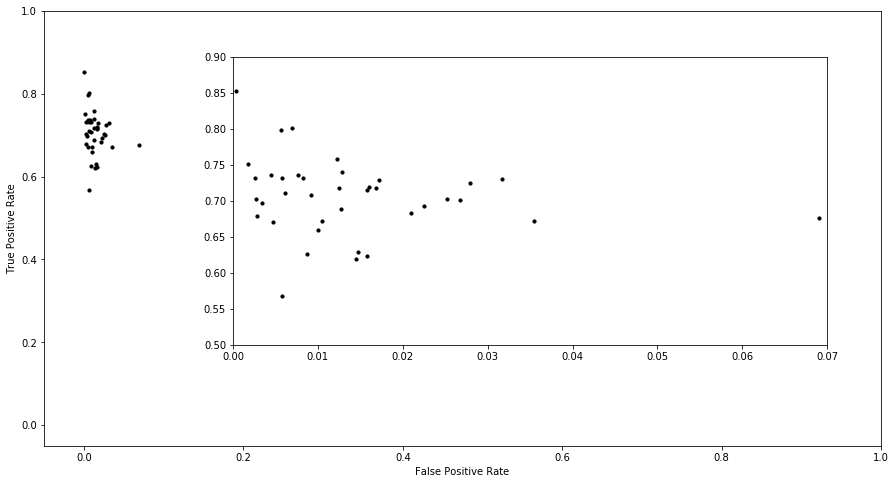
\includegraphics[width=\textwidth]{Figures/dr_fpr_own.png}
	\caption{$\tpr_v$ vs. $\fpr_v$ according to $\Madups$.}
	\label{fig:dr_fpr_own}
\end{figure}

The previous analysis gave us a better understanding on vendors accuracy, but is highly dependent on vendors acknowledging their own errors.
To overcome this dependency, we take a second approach regarding vendors' accuracy, which takes into account our observations from Figure \ref{fig:dups_frequency} and our dataset $\CC$ (instead of $\mathcal{C}_{dups}$), to define another metric $\Mac$.

This new metric $\Mac$ implements a simple minimum/maximum threshold of positive classifications to label a sample as malware/goodware.
Intuitively a sample is classified as goodware according to this metric (\ie\  negative), if every vendor $v\in\mathcal{V}$ classifies it as clean.
To understand if our intuition is sound, we plot Figure~\ref{fig:distribution_clean}, a subset of Figure~\ref{fig:dups_frequency}, showing the frequency $\Pl-\Pf$ for samples that were classified as clean in their first submission (\ie\ samples with $\Pf=0$).
These account for 4,902 samples, 3,741 (76.32\%) of which do not increase in classification.

To arrive at a positive (\ie\ malware) sample definition, we relate Figure \ref{fig:distribution_clean} with Figure \ref{fig:dups_frequency}.
Specifically we want to find a minimum threshold of positive classifications to define a sample as malware.
We chose five as the threshold, observing that percentage of samples that decrease in 5 or more positive classifications is 0.46\%, meaning it is an upper bound for samples that decrease from 5 or more to zero classifications.

\begin{figure}[!htb]
	\centering
	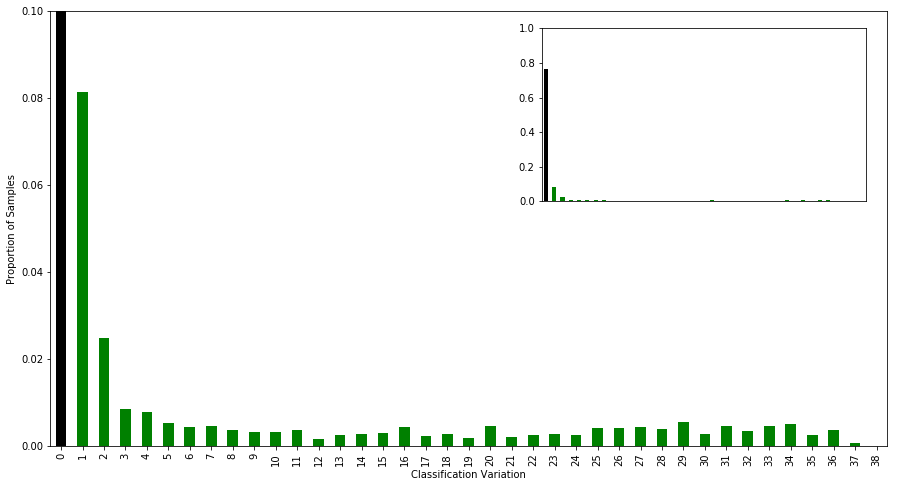
\includegraphics[width=\textwidth]{Figures/distribution_clean.png}
	\caption[Distribution of duplicated samples with $\Pf=0$.]{Distribution of samples that started as goodware and changed in the number of positive classifications between the last and first submission, \ie $\Pl-\Pf$ for samples with $\Pf=0$}
	\label{fig:distribution_clean}
\end{figure}

With these minimum/maximum thresholds for malware/goodware we can now define our new metric $\Mac$ as:

\begin{itemize}
	\item $\tp_v$, \emph{true positive for $v$}, if $v$ and at least 5 other vendors in $\mathcal{V}$ classify it positively;
	\item $\tn_v$, \emph{true negative for $v$}, if $v$ and all other vendors in $\mathcal{V}$ classify it negatively;
	\item $\fp_v$, \emph{false positive for $v$}, if $v$ is the only vendor in $\mathcal{V}$ classifying it positively;
	\item $\fn_v$, \emph{false negative for $v$}, if $v$ classifies it negatively and at least 5 other vendors in $\mathcal{V}$ classify it positively.
\end{itemize}

Having the new metric defined, we again plot each vendors' $\dr_v$ vs.\ $\fpr_v$ according to~$\Mac$, presented in Figure \ref{fig:dr_fpr_d}.
Using this metric we note that vendors' detection rate is more scattered than under $\Madups$, ranging from 20.17\% to 83.50\%, whereas false positive rate is similar, ranging from 0.01\% to 5.77\%.
The scattering along the \tpr\ axis is not surprising, as now we are measuring each vendor $v$ against all others.
What is surprising is the amount of vendors below 50\% detection rate under this metric.
Possible reasoning behind this is either vendors disagree on what is malware (\ie\ \textit{ground truth} problem), or some vendors simply are not good at detecting malware.
As for the \fpr\ axis, it is still interesting to note how the scale remains relatively small, again reflecting the false negative over false positive preference.

\begin{figure}[!htb]
	\centering
	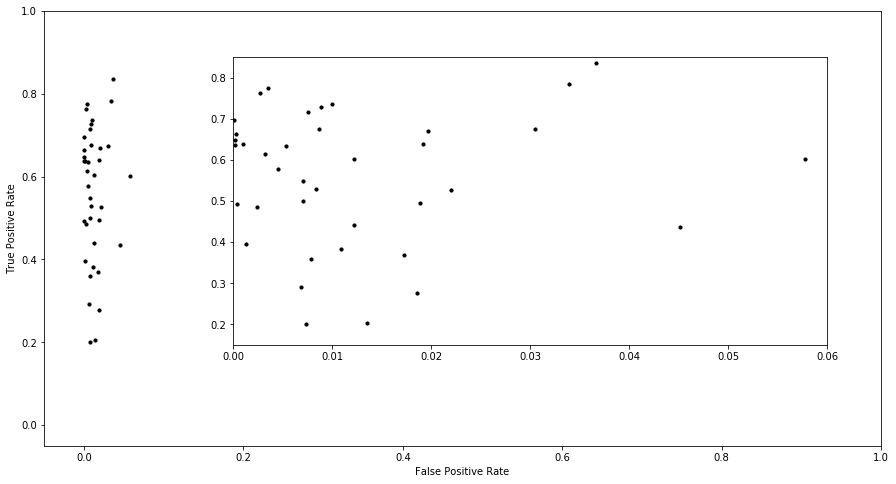
\includegraphics[width=\textwidth]{Figures/dr_fpr_d.png}
	\caption{$\tpr_v$ vs. $\fpr_v$ according to $\Mac$.}
	\label{fig:dr_fpr_d}
\end{figure}

After studying vendors' accuracy under our defined metrics, and given the impossibility of finding a source that is able to unanimously label each sample in our dataset, we want to find the vendors that perform the best under both metrics $\Madups$ and $\Mac$.

Our approach to this problem is to filter the top 20 vendors $\VVdups$ and $\VVc$, according to each metric and define $\VVstar=\VVdups\cap\VVc$.
Given we have to maximize two variables, \tpr\ and \fpr, we decided to take advantage of the linear equation in the form $mx+b=y$ to choose the top vendors.
This form allows us to choose an $m$ and $b$ such that there are 20 vendors above the line, the top vendors $\VVstar$.
By tweaking the variable $m$ one can change the line's steepness, reflecting in a preference between \tpr\ and \fpr\:

\begin{itemize}
	\item \tpr\ preference: $m < 1$, less steepness therefore higher \fpr\ and \tpr\ values;
	\item \fpr\ preference: $m > 1$, more steepness, lower \fpr\ and \tpr\ values.
\end{itemize}

Since we have no \emph{a priori} preference between $\tpr$ nor $\fpr$, we search for the maximum $b$ with $m=1$ such that there are exactly 20 vendors above $x+b=y$ in each graphic (Figures~\ref{fig:dr_fpr_own} and~\ref{fig:dr_fpr_d}).

Figure \ref{fig:dr_fpr_top} shows the $\dr_v$ vs. $\fpr_v$ for the resulting 11 vendors under each metric, $\Madups$ in green and $\Mac$ in red, with $\dr_v$ varying from 63.49\% to 83.50\% and $\fpr_v$ from 0.01\% to 3.67\%.

\begin{figure}[!h]
	\centering
	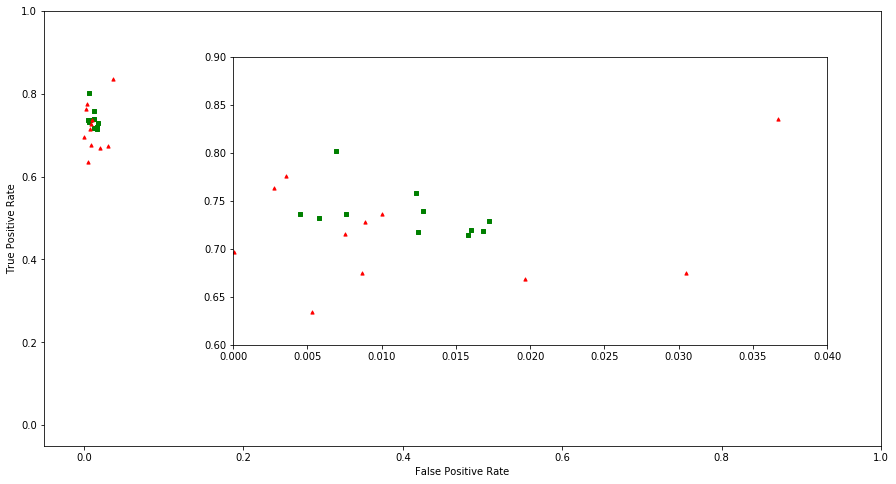
\includegraphics[width=\textwidth]{Figures/dr_fpr_top.png}
	\caption{$\tpr_v$ vs. $\fpr_v$ according to $\Madups$ (green) and $\Mac$ (red).}
	\label{fig:dr_fpr_top}
\end{figure}

With a better understanding on the vendors' accuracy, followed by metrics that allowed us to narrow down the amount of vendors to those that perform best under our metrics, we can now proceed to label our samples as either goodware or malware.

%%%%%%%%%%%%%%%%%%%%%%%%%%%%%%%%%%%%%%%%%%%%%%%%%%%%%%%%%%%%%%%%%%%%%%%%
\section{Data labeling}
\label{section:data_labeling}

Given we are interested not only in providing a model to detect malware, but also in understanding the impacts of \textit{ground truth} in a detection model, we now go into detail on how we made use of the previously defined top vendors $\VVstar$ in conjunction with the information provided by \gls{nsrl} and VirusShare.com to label the available samples.
To do so, we take the previously defined scenarios in Figure \ref{fig:dataset_sizes} to define three labeling metrics.

The first and most real metric we define is $\Mrealv$ that labels a sample $s\in\CC$ as:

\begin{itemize}
	\item $s\in\mal_\real$ if at least 5 vendors in $\VVstar$ classify $s$ positively;
	\item $s\in\good_\real$ if all vendors in $\VVstar$ classify $s$ negatively.
\end{itemize}

Since the labeling information is solely provided by $\VVstar$'s vendors, this metric's ground truth is highly dependent on their performance, which means labeling errors may be present (as we have discussed in \ref{subsection:virustotal_classifications}).
To minimize this dependency, samples between one and four positive classifications are discarded.

\medskip

Our second metric $\Mloosev$, restricts the previous metric $\Mrealv$ to achieve a better ground truth and takes into account the information from \gls{nsrl}, defined by the set $\CNSRL=\NSRL\ \cap\ \CC$, and VirusShare.com, defined by the set $\CVS=\VS\ \cap\ \CC$.

This metric labels a sample $s\in\mathcal{C}$ as:
\begin{itemize}
	\item $s\in\mal_\loose$ if $s\in\mal_\real$ \textbf{and} it belongs to $\CVS$ and does not belong to $\CNSRL$;
	\item $s\in\good_\loose$ if $s\in\good_\real$ \textbf{and} it belongs to $\CNSRL$ and does not belong to $\CVS$.
\end{itemize}
that is
\begin{eqnarray*}
	\mal_\loose&=&\left(\mal_\real\cap\CVS\right)\setminus\CNSRL\\
	\good_\loose&=&\left(\good_\real\cap\CNSRL\right)\setminus\CVS
\end{eqnarray*}

By taking into account the presence in $\NSRL$, that reinforces cleanliness, and VirusShare.com, that reinforces maliciousness, this metric is more reliable, ground truth wise, at the expense of a smaller number of samples.
% (since $\DNSRL \subset\DD$ and $\DVS \subset \DD$).

\medskip

Our third and final metric $\Mstrictv$, is the strictest one, labeling a sample $s\in\CC$ as:
\begin{itemize}
	\item $s\in\mal_\strict$ if all $v\in\VVstar$ classify it positively \textbf{and} $s\in\CVS\setminus\CNSRL$;
	\item $s\in\good_\strict$ if $s\in\good_\loose$.
\end{itemize}

Obviously this is the most reliable metric, in the sense that it is closely related to the samples' ground truth, leaving little room for disagreement. However, this is achieved again at the cost of a smaller number of samples.

Having these three metrics for labeling, we can now proceed to create the datasets for each of these metrics.

%%%%%%%%%%%%%%%%%%%%%%%%%%%%%%%%%%%%%%%%%%%%%%%%%%%%%%%%%%%%%%%%%%%%%%%%
\section{Dataset creation}
\label{section:dataset_creation}

Taking the previously defined metrics, the task of creating labeled datasets based on them is trivial.
We apply each of the previously defined metrics, $\Mstrictv$, $\Mloosev$ and $\Mrealv$ to our classified dataset $\CC$ to obtained three new datasets, $\CC_{strict}\subseteq\CC_{loose}\subseteq\CC_{real}\subseteq\CC$.
Table \ref{tab:dataset_sizes} provides information regarding the size and number of malware and goodware in each of our datasets.

\begin{table}[!htb]
	\renewcommand{\arraystretch}{1.2} % more space between rows
	\centering
	\begin{tabular}{lccc}
		\toprule
		Dataset			& $\CC_{real}$ & $\CC_{loose}$ & $\CC_{strict}$	\\
		\midrule
		Malware			& 0 & 0 & 0\\
		Goodware		& 0 & 0 & 0\\
		\midrule
		Total			& 0 & 0 & 0\\
		\bottomrule
	\end{tabular}
	\caption{Sizes for datasets $\CC_{real}$, $\CC_{loose}$ and $\CC_{strict}$.}
	\label{tab:dataset_sizes}
\end{table}

\medskip

In this chapter we analyzed our available data in order to better understand its advantages and disadvantages.
We provided information regarding our data sources and how the extraction process was made, followed how a simple high level analysis provided interesting insights on the available data.

We took some time understanding how vendors classified reports, how they changed their classifications and how it could impact the reliability of our labels - so much so we defined different metrics that provide different levels of \textit{ground truth} reliability.

Out of these metrics we created three datasets, all subsets of $\CC$, in hopes of enlightening the impacts of \textit{ground truth} when it comes to the task of detecting malware. We are now ready to make use of the datasets to build a malware detection model, which will take place in the following chapters.
 % file "Thesis_Data_Collection.tex"
\cleardoublepage

%%%%%%%%%%%%%%%%%%%%%%%%%%%%%%%%%%%%%%%%%%%%%%%%%%%%%%%%%%%%%%%%%%%%%%%%
%                                                                      %
%     File: Thesis_Static_Features.tex                                 %
%     Tex Master: Thesis.tex                                           %
%                                                                      %
%     Author: João C. Godinho                                          %
%     Last modified : Apr 2018                                         %
%                                                                      %
%%%%%%%%%%%%%%%%%%%%%%%%%%%%%%%%%%%%%%%%%%%%%%%%%%%%%%%%%%%%%%%%%%%%%%%%

\chapter{Static Features}
\label{chapter:static_features}

In the present chapter we go into details about how we built a machine learning model to detect malware based on static features.
We start by detailing the model selection and its evaluation, followed by the selected features.
We finish off by providing how our model performed under various scenarios.

%%%%%%%%%%%%%%%%%%%%%%%%%%%%%%%%%%%%%%%%%%%%%%%%%%%%%%%%%%%%%%%%%%%%%%%%
\section{Model Selection and Evaluation}
\label{section:model_selection_evaluation}

In this section we go over the classifier used to create the model that separates malware from goodware, as well as our evaluation methodology.

%%%%%%%%%%%%%%%%%%%%%%%%%%%%%%%%%%%%%%%%%%%%%%%%%%%%%%%%%%%%%%%%%%%%%%%%
\subsection{Model Selection}
\label{section:model_selection}

Our main concerns when choosing a classifier regard the ability to produce a probabilistic output (\ie\ probability of being malware), good scaling for large number of features and samples and ease of use.

Taking into consideration the guidelines given in~\cite{rossow:practices,shabtai:survey} and related work in~\cite{miller:rev_int,nissim:al_pdf,rieck:dynamic,schultz:data_mining}, we decide to use \textit{\acrfull{lr}} as our model.
This model fits our needs as it gives the probability of a random variable $X$ being 0 or 1, given a set of constraints (\ie~features), scales well with samples and features and it is readily available from several libraries, facilitating implementation~\cite{friedman2001elements}.

\gls{lr} can be defined with the form
\begin{eqnarray*}
	\rho(x) = \dfrac{1}{1 + e^{-x}},&x = \beta_0 + \beta_1x_1 + ... + \beta_nx_n
\end{eqnarray*}
where $\beta_n$ is the learned weight for feature $x_n$.
This weight is learned through iteration in order to minimize the error between the predicted values and the actual values.
In other words, given an \textit{n-th} dimensional set of features, \gls{lr} will try to create an hyperplane that divides samples from two classes.

As \gls{lr} is based on the logistic function (or sigmoid function, visually represented in Figure \ref{fig:sigmoid_function}), each feature $x_n$ can vary from $-\infty$ to $+\infty$ and still the output is contained between 0 and 1, hence providing probabilistic values.

\begin{figure}[!h]
	\centering
	\begin{tikzpicture}
	\begin{axis}
	\addplot[
		color=red,
		domain=-5:5
	]
	{1/(1+exp(-x))};
	\addlegendentry{$1/(1+e^{-x})$}
	\end{axis}
	\end{tikzpicture}
	\caption{Sigmoid function $f(x)=\dfrac{1}{1+e^{-x}}$}
	\label{fig:sigmoid_function}
\end{figure}

To implement this model we take advantage of scikit-learn~\cite{tool:sklearn} library, a Python library that provides a multitude of models and tools that facilitate the creation of \gls{ml} models.

%%%%%%%%%%%%%%%%%%%%%%%%%%%%%%%%%%%%%%%%%%%%%%%%%%%%%%%%%%%%%%%%%%%%%%%%
\subsection{Evaluation}
\label{section:evaluation}

With regards to our evaluation methodology, as we have previously mentioned, our purpose is to understand how laboratory conditions compare to real-world conditions.
We now detail how we achieve and compare these conditions.

Given the purpose of our work, we choose to measure our results by plotting an \gls{auroc} graph, which measures the \tpr~at different \fpr~levels, metrics that are commonly used across similar work~\cite{miller:rev_int,nissim:al_pdf,schultz:data_mining}.

Our first evaluation methodology is to apply a common \gls{ml} validation technique named \textit{k-fold cross-validation}, with $k=10$, depicted in Figure \ref{fig:xval}.
This method works by splitting the dataset into $k$ equally sized parts (folds) and then trains using $k-1$ folds, using the remaining fold as validation.
This process is repeated $k$ times, guaranteeing that every fold is used at least once for validation.
This methodology is useful to prevent over-fitting, as the validation fold is never used together with the training folds.

\begin{figure}[!htb]
	\centering
	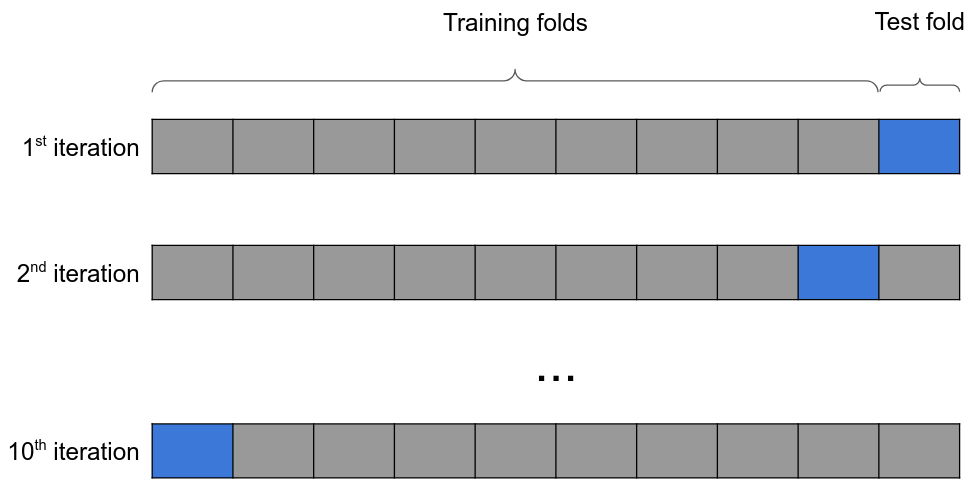
\includegraphics[width=0.8\textwidth]{Figures/dia_xvalidation.png}
	\caption[Cross-validation evaluation example.]{Cross-validation evaluation example with $k=10$ folds.}
	\label{fig:xval}
\end{figure}

This evaluation methodology is our baseline, hence we define it as our \textit{laboratory} conditions, where no time based consistency is taken into account.

\medskip

Although the cross-validation methodology enables to measure the generalization capabilities of a model, it does not account for temporal ordering of the samples.
Since we want to measure the when training samples predate validation, we now define a couple of temporal based validations, based on the concept of cross-validation:

\paragraph{\textit{Past-to-Present}:} This validation, depicted in Figure \ref{fig:past_present}, can be resumed as an iterative methodology where the validation set is a fixed percentage of dataset's most recent samples, whereas the training set is a fixed percentage of the dataset's oldest.
The training set is split into $k$ temporal consistent folds and at each iteration it is extended with more recent folds and scored against the training set, until all folds are used.

\begin{figure}[!htb]
	\centering
	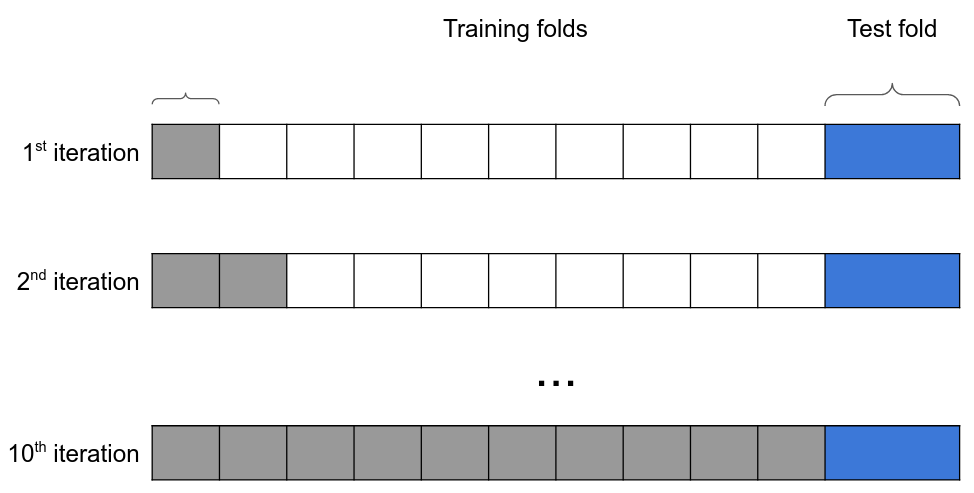
\includegraphics[width=0.8\textwidth]{Figures/dia_pastpresent.png}
	\caption[Past-to-Present evaluation example.]{Past-to-Present evaluation example with 20\% test, 80\% training, $k=10$ folds in training.}
	\label{fig:past_present}
\end{figure}

\paragraph{\textit{Present-to-Past}:} This validation, depicted in Figure \ref{fig:present_past}, is the opposite of \textit{Past-to-Present} with regards to the starting point of the training set.
Again the validation is fixed at the most recent samples, but the training set starts with the temporally closest fold to the validation set.
At each iteration the training set is extended, this time with older folds, and scored against the validation, until all folds are used.

\begin{figure}[!htb]
	\centering
	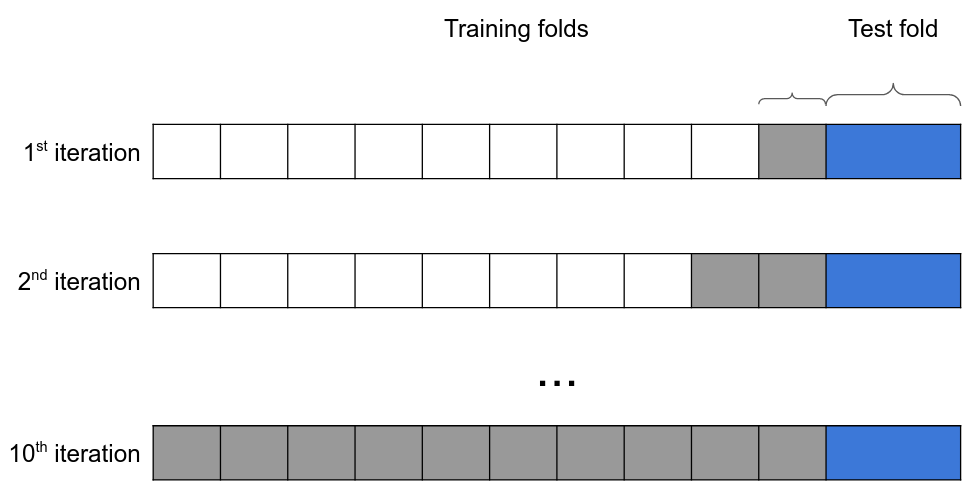
\includegraphics[width=0.8\textwidth]{Figures/dia_presentpast.png}
	\caption[Present-to-Past evaluation example.]{Present-to-Past evaluation example with 20\% test, 80\% training, $k=10$ folds in training.}
	\label{fig:present_past}
\end{figure}

\medskip
Both \textit{Past-to-Present} and \textit{Present-to-Past} validations require two parameters: the size of the validation set and how the increments to the training set are made.
For the purpose of our work, we use the 20\% most recent samples for validation, and split the remaining 80\% into 10 folds, hence the validation is done 10 times, with each iteration increasing the training set size by one fold.

These two validation methodologies give us the ability to account for temporal consistency.
Moreover, they enable us to compare the importance of older \textit{vs.}\ newer samples to classify recent samples.

\paragraph{\textit{Temporal Window}:} This validation, depicted in Figure \ref{fig:sliding_window}, also splits the dataset into $k$ folds, but takes $w$ temporal consistent and contiguous folds (\ie each fold immediately precedes the next one), using the first $w-1$ folds for training (older samples) and the remaining fold (more recent samples) for validation.
By starting with the $w$ first folds of the dataset and sliding one fold on each iteration, we apply a sliding window of size $w$ over the dataset.
For this last validation methodology, we again split the dataset into 10 folds.
The sliding window size $w$, is chosen during the results phase, as its choice depends on previous results.

\begin{figure}[!htb]
	\centering
	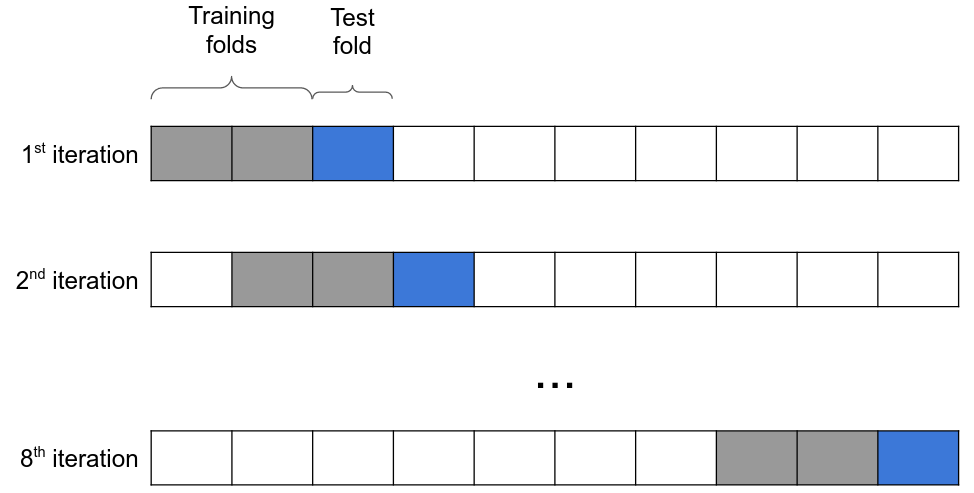
\includegraphics[width=0.8\textwidth]{Figures/dia_slidingwindow.png}
	\caption[\textit{Temporal Window} evaluation example.]{\textit{Temporal Window} evaluation example with $w=3$ window size over $k=10$ folds.}
	\label{fig:sliding_window}
\end{figure}

\medskip

As we have previously described in Section \ref{section:dataset_creation}, we possess 3 different datasets, created from 3 different scenarios.
With that in mind, all our previously described methodologies: cross-validation, past-to-present and present-to-past; are applied to each of the 3 datasets.

Applying the aforementioned methodologies to our 3 datasets enables us to study not only how temporal consistency impacts the results, but also the impact of \textit{ground-truth}.

%%%%%%%%%%%%%%%%%%%%%%%%%%%%%%%%%%%%%%%%%%%%%%%%%%%%%%%%%%%%%%%%%%%%%%%%
\section{Feature Selection}
\label{section:feature_selection}

One of the most important stages in Machine Learning is the selection of the features to analyze, and features based on static imports have shown promising results in \gls{ml} applications for malware detection~\cite{miller:rev_int,schultz:data_mining}.
In this section we describe the adopted static features that were fed into our model.

Although Cuckoo provides enormous amounts of usable information, we chose to start with simple features as to have a basic understanding of how doable our approach is.
More so, one of our main concerns is how the same feature gives different results under our different scenarios, hence the performance between scenarios and methodologies is more relevant than absolute performance.
With that in mind, we chose to use the static imports as features.

Static imports are present in the import table, referencing libraries or other executables that are not part of the current binary.
Their usage is key, as they provide access to all kind of system level operations (\eg\ file manipulation, network access). Given their purpose, our expectation is that a sample's maliciousness can be inferred based on the static imports.

Using Celery~\cite{tool:celery}, a distributed task queue for Python, we optimized the parsing of the available HTML reports, extracting samples that contained information regarding static imports into a new set $\FF_{static}$.
We then joined the samples with static imports $\FF_{static}$ to the labeled samples $\CC_{real}$, obtaining a total of 155,057 labeled samples with static imports $\DD_{static} = \CC_{real} \cap \FF_{static}$.

We then vectorized imports by creating a binary vector where each position corresponds to a specific import.
If a given import $i$ is present in a sample, its feature vector $x$ will have the value 1 at that position $x_i$.
Likewise, if a given import $j$ is not present in a sample, its feature vector $x$ will have the value 0 at that position $x_j$.

Due to the amount of samples and variety of imports, each sample got a vector $x$ of 7,280 dimensions (\ie\ there are 7,280 different imports).
To reduce this number, and to remove any noise due to incorrect parsing of static imports by Cuckoo, we applied a variance threshold.

The variance threshold calculates the variance for each import, removing those that are below a given threshold.
In our case, since we are working with a binary vector, each import can be represented as Bernoulli random variable, hence their variance is given by $p(1-p)$.
With that in mind, we removed any import that did not vary in more than 99\% of samples.

The resulting dataset $\DD_{static}$ got reduced to 153,374 samples, each with a 64 dimensional binary vector.

%%%%%%%%%%%%%%%%%%%%%%%%%%%%%%%%%%%%%%%%%%%%%%%%%%%%%%%%%%%%%%%%%%%%%%%%
\section{Single Layer Results}
\label{section:single_layer_results}

Having met all the necessary conditions to build a \gls{ml} model: model selection and evaluation and feature selection, we are now ready to provide the results of our first experiments.

Using an Ubuntu Virtual Machine with 16 cores and 16GB of RAM, provided by INOV - Inesc Inovação, and taking advantage of scikit-learn~\cite{tool:sklearn} to train the models, Pandas~\cite{tool:pandas} for data analysis and Jupyter Interactive Notebooks~\cite{tool:jupyter} to interact with the Python scripts, we now detail our logistic regression model results.

We define this our single layer model $\LR$ results, as we are directly taking a set of features (static imports in this case) and outputting the probability of a sample being malware.

\medskip
%%%%%%%%%%%%%%%%%%%%%%%%%%%%%%%%%%%%%%%%%%%%%%%%%%%%%%%%%%%%%%%%%%%%%%%%
% \subsection{Laboratory Conditions}
% \label{section:single_layer_laboratory}

We start with what we define as \textit{laboratory conditions}, ideal conditions for the problem of malware detection.
These conditions are met when we take the labeled dataset $\CC_{strict}$ and features $\DD_{static}$, providing scenario $\mathcal{S}_{\strict}$.

Using cross-validation, our $\LR$ scored with an \gls{auroc} of 91\%, as shown by the red curve in Figure \ref{fig:xval_results}.
We argue that such high values are easily attained from factors like a small and reliable dataset, and the use of cross-validation, which mixes samples and ignores possible dependencies on malware samples.

When we relax our ideal conditions to more \textit{real-world conditions}, by testing the labeled dataset $\CC_{loose}$ and $\CC_{real}$ on features $\DD_{static}$ for scenarios $\mathcal{S}_{loose}$ and $\mathcal{S}_{real}$, respectively, the score under \gls{auroc} decreases to 90\% for $\mathcal{S}_{loose}$ (blue curve in Figure \ref{fig:xval_results}) and 75\% for $\mathcal{S}_{real}$ (green curve in Figure \ref{fig:xval_results}).

\begin{figure}[!htb]
	\centering
	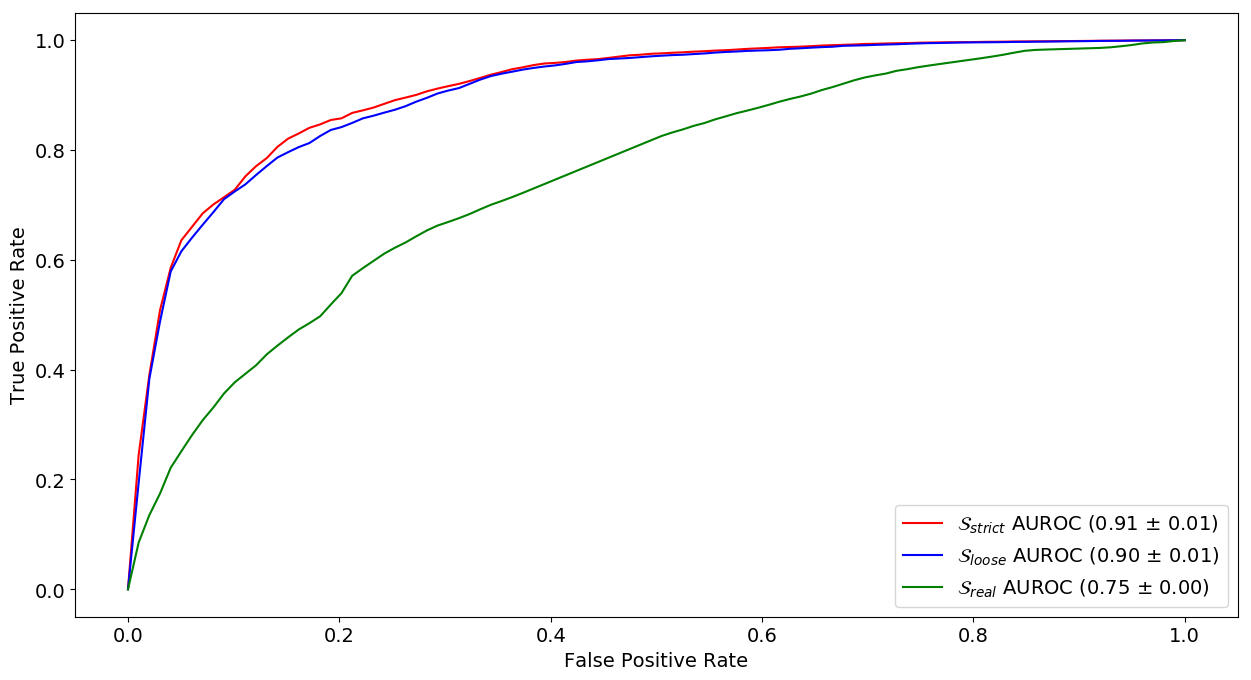
\includegraphics[width=0.8\textwidth]{Figures/xval_results.png}
	\caption[Single layer results for static features in laboratory conditions.]{Single layer results for static features in laboratory conditions.}
	\label{fig:xval_results}
\end{figure}

From $\mathcal{S}_{\strict}$ to $\mathcal{S}_{\loose}$, the only change is the amount of malware labeled samples, which significantly increase.
The difference is interesting, as although the number of malware labeled samples increase significantly, the results are not that affected.
This suggests that although the reliability for malware decreases, its impact is not as noticeable as expected.
This might also suggest that vendors do converge on their definition of malware, under our $\Mloosev$ metric.
If vendors did not converge on what is malware, adding more samples would culminate in worse results, as separation between malware and goodware would become harder.

When looking at the changes from $\mathcal{S}_{\loose}$ to $\mathcal{S}_{\real}$, not only the amount of malware labeled samples increase, but also the number of goodware labeled samples, both by a significant amount. 
The way this impacts the results is pretty significant, as we observe a high decrease in the \gls{auroc} for both models.
The metric $\Mrealv$ that labels malware and goodware for this scenario $\mathcal{S}_{\real}$ disregards the cross-check from outside repositories, which in turn degrade the reliability significantly, as well as increase the dataset size notably.
We attribute the results' degradation mainly to the unreliability of goodware labeling, not only because we have previously seen that increase in malware does not significantly impact results (from $\mathcal{S}_{\strict}$ to $\mathcal{S}_{\loose}$), but also due to the tendency for false negatives in vendors (Figure \ref{fig:dups_frequency}), which in turn lead us to incorrectly label goodware for the samples in $\CC_{real}$.

The results we described show how relaxing \textit{laboratory conditions} to more \textit{real-world conditions} degrade the model's performance.
We now focus on using our previously defined temporal based methodologies to further converge into a real-world scenario.

\medskip

We start by applying our \textit{Past-to-Present} validation to the three scenarios, $\mathcal{S}_{\strict}$, $\mathcal{S}_{\loose}$ and $\mathcal{S}_{\real}$.
As previously defined, this validation starts with an older set of training samples and iteratively adds newer samples, validating each iteration on a fixed set of the most recent samples.
Since our interest is to measure performance variation over time, we plot in Figure~\ref{fig:pastpresent} the \gls{auroc} at every iteration (\ie, fold), for each of our three scenarios.

\begin{figure}[!htb]
	\centering
	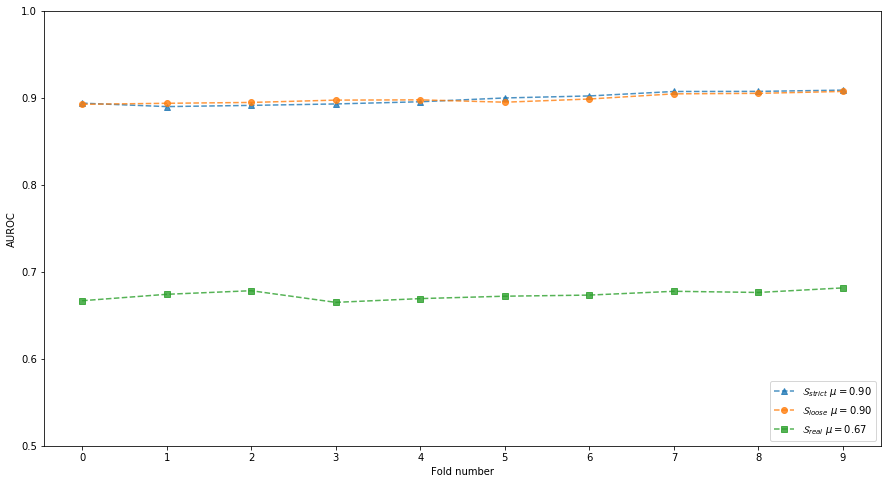
\includegraphics[width=0.8\textwidth]{Figures/pastpresent.png}
	\caption[Single layer results for static features in \textit{Past-to-Present}.]{\gls{auroc} for each iteration of the \textit{Past-to-Present} evaluation. Folds order consistent with temporal order (\ie\ fold 0 contains older samples than
fold 1)}
	\label{fig:pastpresent}
\end{figure}

When directly comparing the average \gls{auroc} for cross-validation and our \textit{Past-to-Present} validation, we note that for both $\mathcal{S}_{\strict}$ and $\mathcal{S}_{\loose}$ the \gls{auroc} remains identical, while for $\mathcal{S}_{\real}$ the score decreases from 0.75\% to 0.68\%.

For both $\mathcal{S}_{\strict}$ and $\mathcal{S}_{\loose}$ we note only a slight increase as new folds are added.
They still relate, as we have previously noted for cross-validation, arguably given their metrics $\Mstrictv$ and $\Mloosev$ are not very different.
The small variation to the cross-validation methodology can be justified by using small dataset size for both cases.

As for $\mathcal{S}_{\real}$ we note higher variation and lower overall score, as the reliability of the metric $\Mrealv$ goes down.
This is expected, not only because we are enforcing temporal consistency between samples, but as new folds are added, the training gets bigger, while the test remains the same.

Our main observation for this validation methodology is that there is a slight tendency for \gls{auroc} to increase, as we move forward in time, close to the validation set.

\medskip

Our next result, which uses our \textit{Present-to-Past} validation methodology will further help analyze the aforementioned detail.
The \textit{Present-to-Past} validation enhances the previous results under real-world conditions.
This methodology starts by fixing the validation set to the most recent samples, but with the training set starting at the temporally closest samples to validation.
At each iteration, older samples are added to the training set and validated on the fixed, most recent, samples.

By applying this methodology to the three scenarios, $\mathcal{S}_{\strict}$, $\mathcal{S}_{\loose}$ and $\mathcal{S}_{\real}$, we plot Figure \ref{fig:presentpast}, where the X axis increases as older samples are added to the training set (\ie\ fold 0 contains newer samples than fold 1), hence measuring the performance variance over time.
Similarly to the previous observation, the average \gls{auroc} remains identical when compared to cross-validation for both $\mathcal{S}_{\strict}$ and $\mathcal{S}_{\loose}$.
As for $\mathcal{S}_{\real}$, we note a decrease in score from 75\% to 69\%.

\begin{figure}[!h]
	\centering
	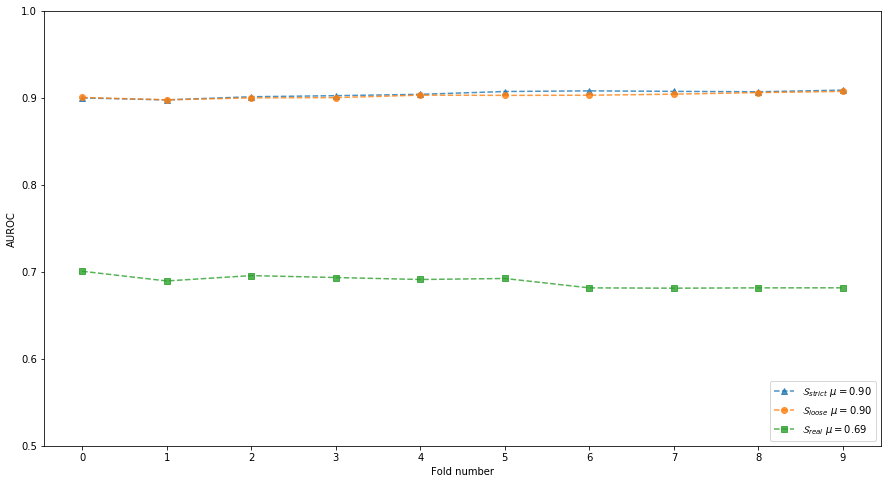
\includegraphics[width=0.8\textwidth]{Figures/presentpast.png}
	\caption[Single layer results for static features in \textit{Present-to-Past}.]{\gls{auroc} for each iteration of the \textit{Present-to-Past} evaluation. Folds order is the inverse of temporal order (\ie\ fold 0 contains newer samples than fold 1)}
	\label{fig:presentpast}
\end{figure}

The comparison between scenarios is identical to what was observed in cross-validation and \textit{Past-to-Present}: scenarios $\mathcal{S}_{\strict}$ and $\mathcal{S}_{\loose}$ display very similar results, with $\mathcal{S}_{\real}$ dropping behind due to its less reliable labeling metric.
It is noticeable that using the entire dataset does not bring much improvement to the final results. In fact, for $\mathcal{S}_{\real}$ the score even drops after fold $\#2$.

With these results, our original observation that samples closer to the validation set benefit the model becomes more convincing. In fact, we argue that there should be an ideal number of necessary training folds, temporally consistent with the validation fold (\ie\ any fold from training predates validation), needed to maximize the overall score.

\medskip

Finally, we analyze how does such reduced training set behaves in our scenarios; for this purpose, we define a sliding window that moves forward in time through each scenario for training and validation.
We propose a reduction on the training size to $w=3$ folds predating the validation fold. We choose $w=3$, since we have seen that the scores either do not improve (for $\mathcal{S}_{\strict}$ and $\mathcal{S}_{\loose}$) or actually go down (for $\mathcal{S}_{\real}$) with higher folds.
In summary, we have selected 30\% of each dataset for training purposes and the next 10\% for validation (3 training folds, 1 validation fold), and then started moving the window forward in time (1 fold at a time) to obtain the following results (Figure~\ref{fig:slidingwindow}): for  $\mathcal{S}_{\strict}$, $\mathcal{S}_{\loose}$ and $\mathcal{S}_{\real}$, we obtain \gls{auroc} values of 89\%, 88\% and 73\%, respectively. 
These results come to reaffirm our argument that we can reduce the size of the training set, without losing any significant score (2\% for each scenario).

\begin{figure}[!h]
	\centering
	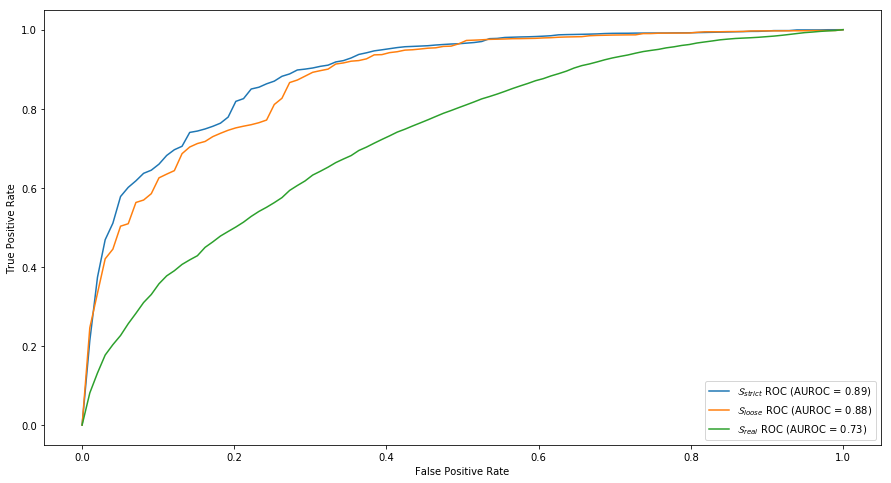
\includegraphics[width=0.8\textwidth]{Figures/slidingwindow.png}
	\caption[Single layer results for static features in \textit{Temporal Window}.]{\gls{auroc} for our three scenarios, under the \textit{Temporal Window} methodology.}
	\label{fig:slidingwindow}
\end{figure}

Comparing these results with the baseline cross-validation, we note a decrease for each scenario, specifically a decrease from 91\% to 89\% for $\mathcal{S}_{\strict}$, from 90\% to 88\% for $\mathcal{S}_{\loose}$ and from 75\% to 73\% for $\mathcal{S}_{\real}$.
We should highlight that the results that use temporal consistency should better reflect the reality than standard cross-validation, since we are requiring temporally ordered samples.
Another important idea that should be stressed is that for cross validation we used a fairly reasonable amount of data for training purposes, whereas in this last case we used a restricted amount of data. This might be a relevant issue in a few year's time. The results obtained are summarized in Table \ref{tab:singlelayer_results}.

\begin{table}[!htb]
	\renewcommand{\arraystretch}{1.2} % more space between rows
	\centering
	\begin{tabular}{ccccc}
		\toprule
		AUROC & $\DS_\strict$ & $\DS_\loose$ & $\DS_\real$ & Train/Test \%\\
		\midrule
		Cross-Validation & 0.91 & 0.90 & 0.75 & 90 / 10\\
		Past-to-Present & 0.90 & 0.90 & 0.67 & 10 to 90 / 10\\
		Present-to-Past & 0.90 & 0.90 & 0.69 & 10 to 90 / 10\\
		Sliding-Window & 0.89 & 0.88 & 0.73 & 30 / 10\\
		\bottomrule
\end{tabular}
\caption{Single layer results summary.}
\label{tab:singlelayer_results}
\end{table}

\medskip

With a better understanding of how the model behaves under different methodologies, we now diverge to how we improved not only the overall results, but also the information provided by the model.
 % file "Thesis_Static_Features.tex"
\cleardoublepage

%%%%%%%%%%%%%%%%%%%%%%%%%%%%%%%%%%%%%%%%%%%%%%%%%%%%%%%%%%%%%%%%%%%%%%%%
%                                                                      %
%     File: Thesis_Model_Improvements.tex                              %
%     Tex Master: Thesis.tex                                           %
%                                                                      %
%     Author: João C. Godinho                                          %
%     Last modified : Apr 2018                                         %
%                                                                      %
%%%%%%%%%%%%%%%%%%%%%%%%%%%%%%%%%%%%%%%%%%%%%%%%%%%%%%%%%%%%%%%%%%%%%%%%

\chapter{Model Improvements}
\label{chapter:model_improvements}

Having a solid baseline model for our malware detection task together with how laboratory \textit{vs.}\ real-world scenarios change the model outcome, we now take this chapter to present the improvements made in order to obtain a more robust model to detect malware.
We start by describing our first improvement, applying a multi layer model to extract more information regarding a sample.
We then take this enhanced model and increase the number of features to include dynamic content and how it impacted the model's results.

%%%%%%%%%%%%%%%%%%%%%%%%%%%%%%%%%%%%%%%%%%%%%%%%%%%%%%%%%%%%%%%%%%%%%%%%
\section{Multi Layer Model}
\label{section:improvements_multi_layer}

On the previous chapter we ended up with a simple \gls{lr} model $\LR$ that given a set of static imports from a sample, would give the probability of it being malware.
Although that was the end purpose of our work, it does not give any deeper understanding of the sample, other than being or not malware.
With that in mind, we propose a new model that not only provides the probability of a sample being malware, but also the probability of being from a specific malware type.

This new model $\mathcal{E}$ comprises a simple ensemble stacking approach, which instead of using a single \gls{lr} classifier, multiple ones are used, layered into two steps.

The first step (layer $\mathcal{E}_{\mathcal{L}_{0}}$) is composed of $n$ \gls{lr} models, where $n$ is the number of possible classes.
Each model is trained to output the likelihood of sample belonging to one of the $n$ classes, in a \textit{one-vs-all} methodology (\ie\ a sample either belongs to $\mathcal{C}_{n}$ or not), having as input the raw features (\eg\ static imports).

The second step (layer $\mathcal{E}_{\mathcal{L}_{1}}$) is identical to $\mathcal{LR}$, but now takes as features the output of each classifier from the previous layer, outputting the likelihood of a sample being malware.

In summary, as depicted in Figure \ref{fig:dia_multilayer}, we define a 2 layer ensemble stacking with $n$ classifiers on the first layer to a single classifier in the second layer.

\begin{figure}[!htb]
	\centering
	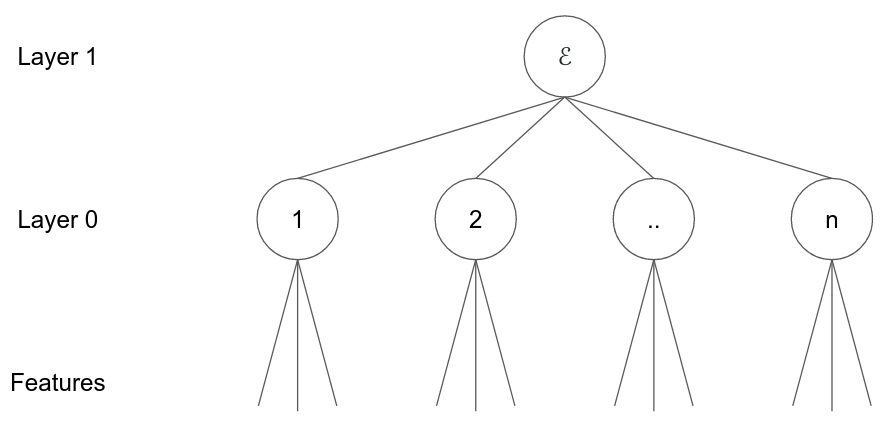
\includegraphics[width=0.8\textwidth]{Figures/dia_multilayer.png}
	\caption{Multi layer model representation.}
	\label{fig:dia_multilayer}
\end{figure}

%%%%%%%%%%%%%%%%%%%%%%%%%%%%%%%%%%%%%%%%%%%%%%%%%%%%%%%%%%%%%%%%%%%%%%%%
\subsection{Malware Classes}

With this new model defined, we now present our approach on selecting the $n$ classes of interest.
This represents another labeling problem, but now instead of having to label between goodware and malware, we have to label the malware as belonging to some subclass.

To choose the malware classes for our datasets, we take into account our description in Chapter \ref{chapter:related_work} regarding propagation methods and malware names based on purpose.
With this in mind, we chose 6 malware classes: \textit{virus}, \textit{trojan}, \textit{worm}, \textit{ransom}, \textit{spyware} and \textit{other}.
The first three classes, \textit{virus}, \textit{trojan} and \textit{worm}, were chosen from the propagation methods, whereas \textit{ransom} and \textit{spyware}
where chosen due to their popularity in recent years. The last class, \textit{other}, serves for any malware that does not fit the previous five.

As mentioned in Chapter \ref{chapter:related_work}, there is no agreed upon naming convention for malware, which translates into different names for the same malware sample.
To minimize this problem, we referenced a tool by Sebastián, M. et al.~\cite{sebastian2016avclass}, AVClass, which was built to normalize a malware sample name into the most likely family, using the names provided by VirusTotal~\cite{tool:virustotal}.

We took advantage of this tool and modified it such that instead of providing a family name, it would provide one (or more) of the 6 previously defined classes.
Specifically, we changed it in a way that given a set of malware names, the output would be a distribution over the 6 malware classes.

To calculate each class weight we apply the following formula
\begin{eqnarray*}
	\mathcal{W}_c = \dfrac{f_c}{\sum\limits_{c}f_c}
\end{eqnarray*}

where $f_c$ is the frequency for the class $c$ and $\sum_{c}f_c$ is the number of times all classes appear.
For example, if a given set of names contain the name \textit{trojan} 3 times and the name \textit{virus} one time, then the weights would be
\begin{eqnarray*}
	\mathcal{W}_{trojan}=\dfrac{3}{4}=0.75,~\mathcal{W}_{virus}=\dfrac{1}{4}=0.25,~ \mathcal{W}_{c}=0, c \in \{worm, spyware, other, ransom\}
\end{eqnarray*}

\medskip

Having these malware classes defined for our multi layer model, we also added the \textit{goodware} class for samples that are not malware.
Doing so gives us 7 possible classes, 6 of which are malware only.
It is worth mentioning that if a sample belongs to the \textit{goodware} class, it cannot belong to any other, likewise, if it belongs to any malware class, it cannot belong to the \textit{goodware} class.

By applying this new labeling, we refine our previous datasets $\CC_{strict}$, $\CC_{loose}$ and $\CC_{real}$ as shown in Table \ref{tab:dataset_sizes_new}.

\begin{table}[!htb]
	\renewcommand{\arraystretch}{1.2} % more space between rows
	\centering
	\begin{tabular}{lccc}
		\toprule
		Dataset			& $\CC_{real}$ & $\CC_{loose}$ & $\CC_{strict}$	\\
		\midrule
		Trojan			& 0 & 0 & 0\\
		Virus			& 0 & 0 & 0\\
		Worm			& 0 & 0 & 0\\
		Spyware			& 0 & 0 & 0\\
		Ransom			& 0 & 0 & 0\\
		Other			& 0 & 0 & 0\\
		\midrule
		Total Malware	& 0 & 0 & 0\\
		Total Goodware	& 0 & 0 & 0\\
		\midrule
		\midrule
		Total			& 0 & 0 & 0\\
		\bottomrule
	\end{tabular}
	\caption{New sizes for datasets $\CC_{real}$, $\CC_{loose}$ and $\CC_{strict}$.}
	\label{tab:dataset_sizes_new}
\end{table}

In sum, we added a layer of labeling to our dataset, where a sample can either belong to the \textit{goodware} class, or to a set of the other 6 malware classes.
This concludes the description of our first improvement to the model, what follows are our improvements regarding features.

%%%%%%%%%%%%%%%%%%%%%%%%%%%%%%%%%%%%%%%%%%%%%%%%%%%%%%%%%%%%%%%%%%%%%%%%
\section{Dynamic Features}
\label{section:improvements_dynamic_features}

Having described our first model improvement, we now proceed to our second enhancement, which takes advantage of the amount of information available in Cuckoo's~\cite{tool:cuckoo} reports.

In the previous chapter, we used static imports as features for our malware detection model.
Although the results are reasonable, the information which can be retrieved from static imports alone is limited.
As an example, if a sample is compressed, encrypted or packed, its behavior cannot be inferred from static imports only.
To overcome these limitations, we resort to more dynamic information provided by Cuckoo.

Given that Cuckoo runs the provided samples inside a virtual machine, it monitors the sample from a dynamic point of view.
This monitoring includes information like the sequence of library calls and their categories and network and file activity.
With this in mind, we now detail what dynamic information we extracted from the reports.

%%%%%%%%%%%%%%%%%%%%%%%%%%%%%%%%%%%%%%%%%%%%%%%%%%%%%%%%%%%%%%%%%%%%%%%%
\subsection{Category Calls}
\label{section:improvements_categories}

The first type of dynamic information we extracted were the number of dynamic category calls.
When Cuckoo runs and monitors a sample, it registers some low level library calls, which it then assigns to a fixed number of categories.

There are a total of 14 different categories defined by Cuckoo: \textit{anomaly}, \textit{device}, \textit{filesystem}, \textit{hooking}, \textit{misc}, \textit{network}, \textit{process}, \textit{registry}, \textit{services}, \textit{socket}, \textit{synchronization}, \textit{system}, \textit{threading} and \textit{windows}.
After using Celery~\cite{tool:celery} to extract the number of each category calls for the samples, we obtained a total of 148,036 samples with information regarding category calls.

Figure \ref{fig:boxplot_category_calls} shows a boxplot for the category calls, where one can see the categories \textit{filesystem}, \textit{registry} and \textit{system} are the ones with higher mean, hence more used than the other categories.
Although not depicted, some outliers for the number of category calls go up to 1,400,000, which do not provide useful information other than the number of category calls is very high.

\begin{figure}[!htb]
	\centering
	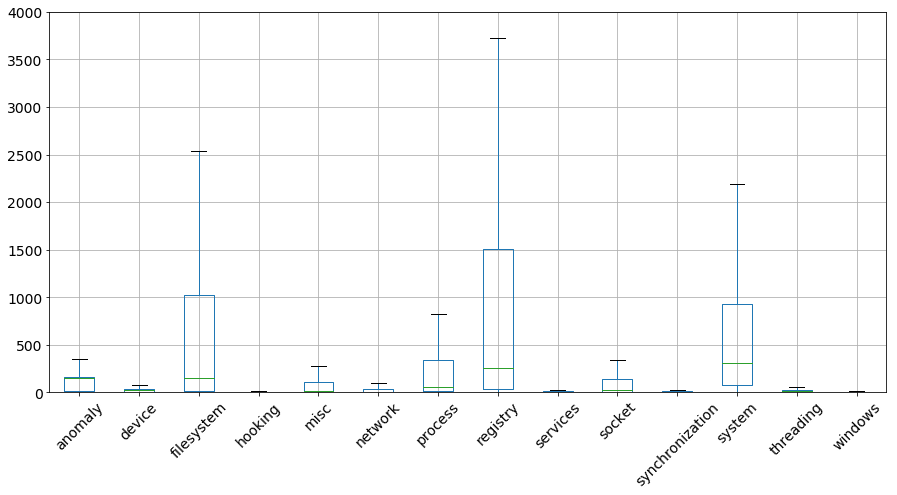
\includegraphics[width=\textwidth]{Figures/boxplot_category_calls.png}
	\caption{Category calls boxplot.}
	\label{fig:boxplot_category_calls}
\end{figure}

With that in mind, we decide to transform the values into a $[0,1]$ range.
We do this by using scikit-learn's~\cite{tool:sklearn} \textit{QuantileTransformer} with a normal distribution, which splits the possible values into bins such that the resulting distribution is of type \textit{Gaussian} with a mean of 0.
This way we have a greater number of bins around the mean, allowing for better discrimination, whereas very large values fall into the same bin.

%%%%%%%%%%%%%%%%%%%%%%%%%%%%%%%%%%%%%%%%%%%%%%%%%%%%%%%%%%%%%%%%%%%%%%%%
\subsection{Library Calls}
\label{section:improvements_api_unigrams}

Our second type of dynamic information are the number of library calls, which closely relate to the previous feature.
While \textit{category calls} provide the number of calls for a given category, \textit{library calls} provide the count for each library call, hence being a subset of the previous.

Cuckoo~\cite{tool:cuckoo} registers the number of calls for 163 different functions, ranging from opening and closing files, to opening and closing sockets.
Again we used Celery~\cite{tool:celery} to extract these numbers, obtaining information from 148,036 samples.

Given we are dealing with a high number of features (163 different library calls), we decided to apply the same variance threshold as in Section \ref{section:feature_selection}, to remove features that do not vary in most samples.
By choosing a threshold of 80\%, we remove library calls that do not vary in more than 80\% of the samples, effectively reducing the number of library calls to 144.
With regards to how these features can vary from 0 to $+\infty$, as before, we again apply a quantile transformer with a normal distribution.

%%%%%%%%%%%%%%%%%%%%%%%%%%%%%%%%%%%%%%%%%%%%%%%%%%%%%%%%%%%%%%%%%%%%%%%%
\subsection{Cuckoo Signatures}
\label{section:improvements_categories}

For our third and last type of dynamic information, we resort to Cuckoo~\cite{tool:cuckoo} custom signatures.
These signatures are built from certain activities that Cuckoo deems malicious or suspicious.
For example, if a sample allocates memory and then makes it executable, it might suggest some sort of packing or obfuscation.

Although some signatures are defined by a sequence of library calls, which could also be attained by creating n-grams of our previously defined feature, using the already defined Cuckoo signatures saves training time.
As an example, creating bi-grams of library calls, given there are 144 unique calls, would yield over 20,000 possible features, hence being unpractical.

To extract these signatures, we use Celery~\cite{tool:celery} and obtain a total of 124,821 samples and 61 different signatures.
As with our static import features, we use a binary vector for each sample, where each position corresponds to a specific signature. Re-iterating on how we represent this, if a given signature $i$ is present in a sample, its feature vector $x$ will have the value 1 at that position $x_i$. Likewise, if a given signature $j$ is not present in a sample, its feature vector $x$ will have the value 0 at that position $x_j$.

\medskip

Having these new features, we create a new set with all features (static, category and library calls and signatures) $\FF_{dynamic}$.
We joined these samples $\FF_{dynamic}$ to the labeled samples $\CC_{real}$, obtaining a total of \miss{size} labeled samples with dynamic imports $\DD_{dynamic} = \CC_{real} \cap \FF_{dynamic}$.

% To reduce the number of features into those that are more representative, we apply, as in other features, a variance threshold, removing signatures that do not vary in more than 80\% of the samples.
% By doing so, we reduce the total number of signatures to 

%%%%%%%%%%%%%%%%%%%%%%%%%%%%%%%%%%%%%%%%%%%%%%%%%%%%%%%%%%%%%%%%%%%%%%%%
\section{Improved Model Results}
\label{section:improvements_results}

In the previous sections we described all our modifications to the original model $\LR$: a two layer approach that splits malware into subclasses and the addition of three dynamic features.
We now present the results of our new model $\mathcal{E}$, validated using the same methodology as described in \ref{section:evaluation}.
Specifically we test the model using the baseline cross-validation methodology, followed by our three temporally consistent scenarios: \textit{Past-to-Present}, \textit{Present-to-Past} and \textit{Temporal Window}.
We test each methodology using the three different scenarios: $\mathcal{S}_{\strict}$, $\mathcal{S}_{\loose}$ and $\mathcal{S}_{\real}$.

We again use the resources provided by INOV - Inesc Inovação, together with scikit-learn~\cite{tool:sklearn}, Pandas~\cite{tool:pandas} and Jupyter Interactive Notebooks~\cite{tool:jupyter} to train and analyze the data.

\medskip

Starting with \textit{laboratory conditions}, we apply the cross-validation evaluation to model $\mathcal{E}$ with the labeled dataset $\CC_{strict}$ and features $\DD_{dynamic}$, providing scenario $\mathcal{S}_{\strict}$.
For this scenario, we obtain an \gls{auroc} of \miss{score}, as presented by the red line in Figure \ref{fig:improved_xval}.
These provide the highest results, provided by factors like a small and reliable dataset, more features and the use of cross-validation.

Relaxing to more \textit{real-world conditions}, under the form of a less reliable ground truth, we test the datasets $\CC_{loose}$ and $\CC_{real}$ on features $\DD_{dynamic}$.
As shown in Figure \ref{fig:improved_xval}, the score under \gls{auroc} decreases to \miss{socre} for $\mathcal{S}_{\loose}$ (blue line) and \miss{score} for $\mathcal{S}_{\real}$ (green line).

\begin{figure}[!h]
	\centering
	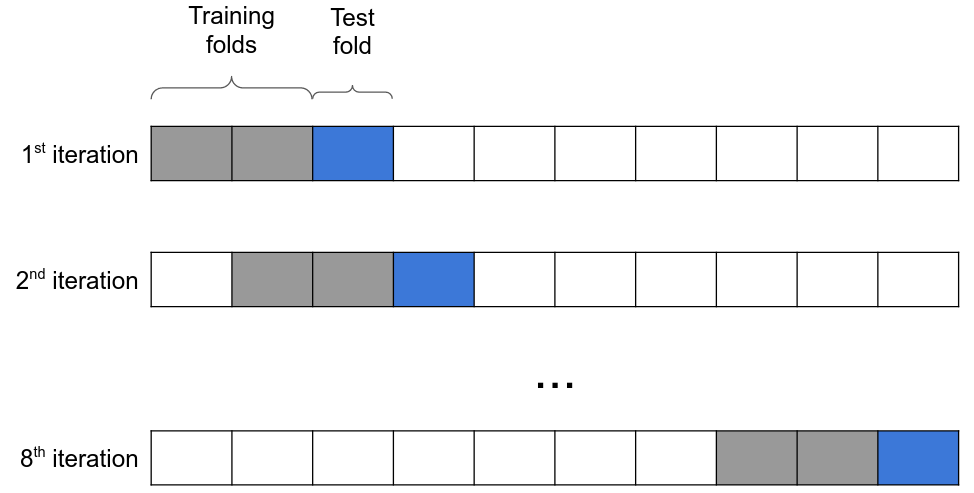
\includegraphics[width=0.8\textwidth]{Figures/dia_slidingwindow.png}
	\caption{Improved model results with dynamic features in laboratory conditions.}
	\label{fig:improved_xval}
\end{figure}

% Adicionar seccao para resultados do multi layer apenas.

As with previous results, one notes that from $\mathcal{S}_{\strict}$ to $\mathcal{S}_{\loose}$ the results are not highly affected, when the change between the scenarios is merely in the number of malware samples.

Between $\mathcal{S}_{\loose}$ to $\mathcal{S}_{\real}$ we again note the already seen pattern, the lowest score when using the most realistic dataset.

\todo[inline]{}

When looking at the changes from $\mathcal{S}_{\loose}$ to $\mathcal{S}_{\real}$, not only the amount of malware labeled samples increase, but also the number of goodware labeled samples, both by a significant amount. 
The way this impacts the results is pretty significant, as we observe a high decrease in the \gls{auroc} for both models.
The metric $\Mrealv$ that labels malware and goodware for this scenario $\mathcal{S}_{\real}$ disregards the cross-check from outside repositories, which in turn degrade the reliability significantly, as well as increase the dataset size notably.
We attribute the results' degradation mainly to the unreliability of goodware labeling, not only because we have previously seen that increase in malware does not significantly impact results (from $\mathcal{S}_{\strict}$ to $\mathcal{S}_{\loose}$), but also due to the tendency for false negatives in vendors (Figure \ref{fig:dups_frequency}), which in turn lead us to incorrectly label goodware for the samples in $\CC_{real}$.

The results we described show how relaxing \textit{laboratory conditions} to more \textit{real-world conditions} degrade the model's performance.
We now focus on using our previously defined temporal based methodologies to further converge into a real-world scenario.

\medskip

We start by applying our \textit{Past-to-Present} validation to the three scenarios, $\mathcal{S}_{\strict}$, $\mathcal{S}_{\loose}$ and $\mathcal{S}_{\real}$.
As previously defined, this validation starts with an older set of training samples and iteratively adds newer samples, validating each iteration on a fixed set of the most recent samples.
Since our interest is to measure performance variation over time, we plot in Figure~\ref{fig:pastpresent} the \gls{auroc} at every iteration (\ie, fold), for each of our three scenarios.

\begin{figure}[!htb]
	\centering
	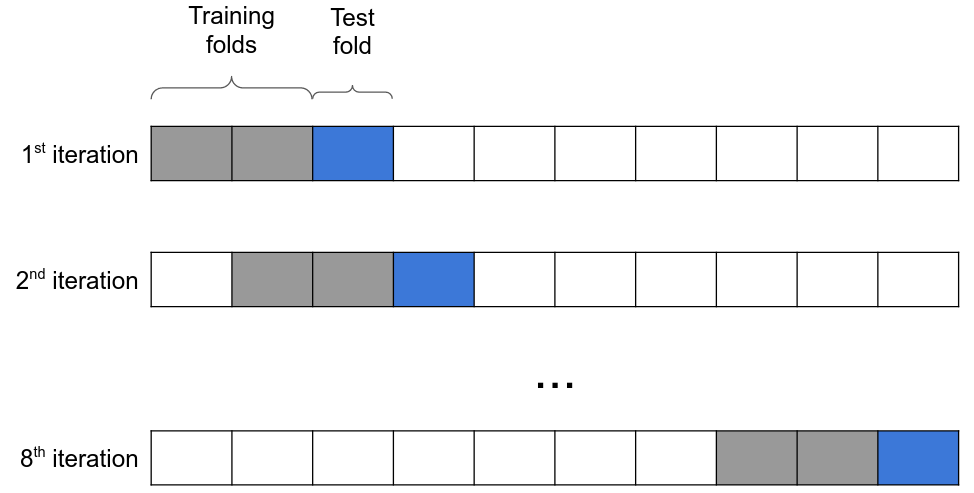
\includegraphics[width=0.8\textwidth]{Figures/dia_slidingwindow.png}
	\caption[Single layer results for static features in \textit{Past-to-Present}.]{\gls{auroc} for each iteration of the \textit{Past-to-Present} evaluation. Folds order consistent with temporal order (\ie\ fold 0 contains older samples than
		fold 1)}
	\label{fig:pastpresent}
\end{figure}

When directly comparing the average \gls{auroc} for cross-validation and our \textit{Past-to-Present} validation, we note a decrease from \miss{score} to \miss{score} for $\mathcal{S}_{\strict}$, \miss{score} to \miss{score} for $\mathcal{S}_{\loose}$, and \miss{score} to \miss{score} for $\mathcal{S}_{\real}$.
This decrease is intuitive to the methodology, as we are forcing temporal consistency between samples.

When looking at results from $\mathcal{S}_{\strict}$ and $\mathcal{S}_{\loose}$, we see they closely relate.
This relation has already been noticed on previous cross-validation results, as their metrics $\Mstrictv$ and $\Mloosev$ are not very different.
As for $\mathcal{S}_{\real}$, the degradation is higher, as the reliability of the metric $\Mrealv$ goes down.

Our main observation for this validation methodology is that there is a slight tendency for \gls{auroc} to increase, as we move forward in time, close to the validation set.

Both $\mathcal{S}_{\strict}$ and $\mathcal{S}_{\loose}$ behave similarly under our \textit{Past-to-Present} evaluation, decreasing the \gls{auroc} until fold \miss{fold}, after which both increase, stabilizing around \miss{score} \gls{auroc} by the last \miss{two} folds. As for $\mathcal{S}_{\real}$, its \gls{auroc} does not vary significantly, although a subtle increase over time is noticeable.

\medskip

Our next result, which uses our \textit{Present-to-Past} validation methodology will further help analyze the aforementioned detail.
The \textit{Present-to-Past} validation enhances the previous results under real-world conditions.
This methodology starts by fixing the validation set to the most recent samples, but with the training set starting at the temporally closest samples to validation.
At each iteration, older samples are added to the training set and validated on the fixed, most recent, samples.

By applying this methodology to the three scenarios, $\mathcal{S}_{\strict}$, $\mathcal{S}_{\loose}$ and $\mathcal{S}_{\real}$, we plot Figure \ref{fig:presentpast}, where the X axis increases as older samples are added to the training set (\ie\ fold 0 contains newer samples than fold 1), hence measuring the performance variance over time.
Similarly to the previous observation, the average \gls{auroc} suffers a decrease when compared to cross-validation. For $\mathcal{S}_{\strict}$ we note a change from \miss{score} to \miss{score}, for $\mathcal{S}_{\loose}$ the decrease is from \miss{score} to \miss{score}, and for $\mathcal{S}_{\real}$ \miss{score} to \miss{score}.

\begin{figure}[!h]
	\centering
	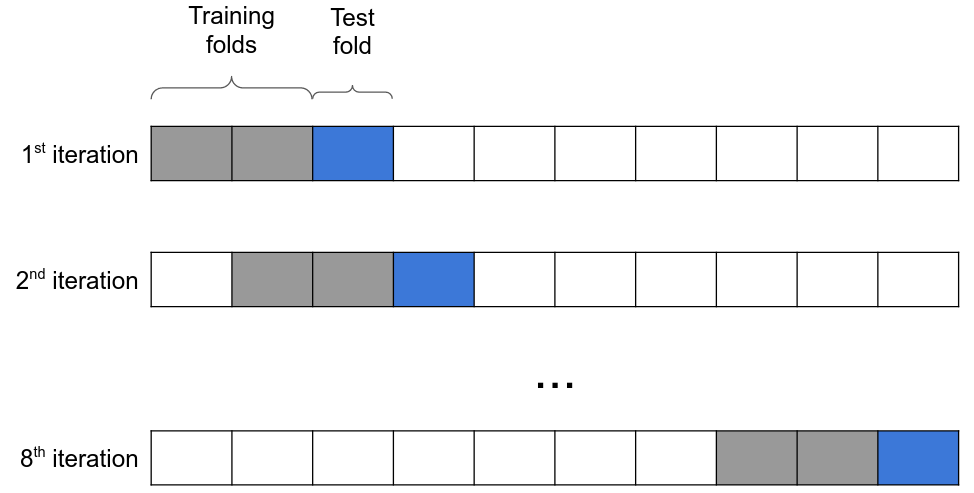
\includegraphics[width=0.8\textwidth]{Figures/dia_slidingwindow.png}
	\caption[Single layer results for static features in \textit{Present-to-Past}.]{\gls{auroc} for each iteration of the \textit{Present-to-Past} evaluation. Folds order is the inverse of temporal order (\ie\ fold 0 contains newer samples than fold 1)}
	\label{fig:presentpast}
\end{figure}

The comparison between scenarios is identical to what was observed in cross-validation and \textit{Past-to-Present}: scenarios $\mathcal{S}_{\strict}$ and $\mathcal{S}_{\loose}$ display very similar results, with $\mathcal{S}_{\real}$ dropping behind due to its less reliable labeling metric.

With these results, our original observation that samples closer to the validation set benefit the model becomes more convincing. In fact, we argue that there should be an ideal number of necessary training folds, temporally consistent with the validation fold (\ie\ any fold from training predates validation), needed to maximize the overall score.

\medskip

Finally, we analyze how does such reduced training set behaves in our scenarios; for this purpose, we define a sliding window that moves forward in time through each scenario for training and validation.
We propose a reduction on the training size to \miss{$w=3$} folds predating the validation fold. We choose \miss{$w = 3$}, since we have seen that the scores either do not improve (for $\mathcal{S}_{\strict}$ and $\mathcal{S}_{\loose}$) or actually go down (for $\mathcal{S}_{\real}$) with higher folds.
In summary, we have selected \miss{30\%} of each dataset for training purposes and the next \miss{10\%} for validation \miss{(3 training folds, 1 validation fold)}, and then started moving the window forward in time (1 fold at a time) to obtain the following results (Figure~\ref{fig:slidingwindow}): for  $\mathcal{S}_{\strict}$, $\mathcal{S}_{\loose}$ and $\mathcal{S}_{\real}$, we obtain \gls{auroc} values of \miss{score, score and score}, respectively. 
These results come to reaffirm our argument that we can reduce the size of the training set, without losing any significant score.

\begin{figure}[!h]
	\centering
	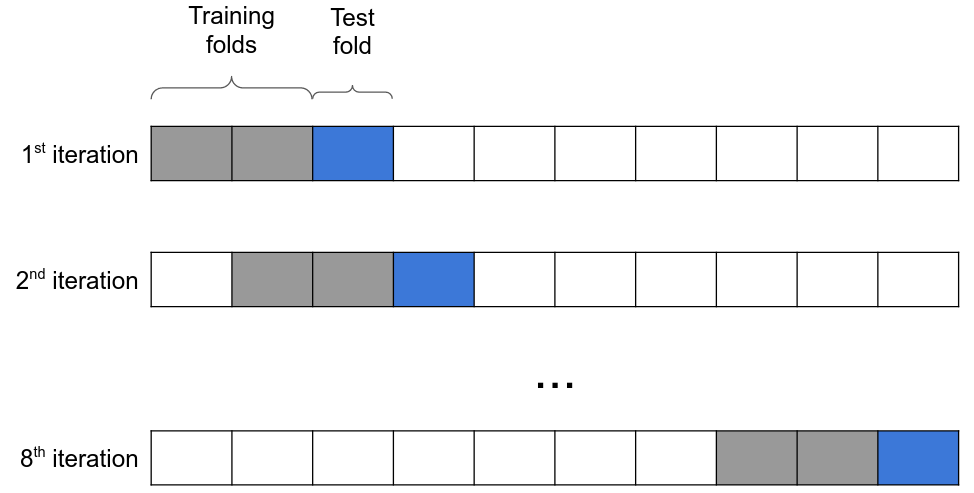
\includegraphics[width=0.8\textwidth]{Figures/dia_slidingwindow.png}
	\caption[Single layer results for static features in \textit{Temporal Window}.]{\gls{auroc} for our three scenarios, under the \textit{Temporal Window} methodology.}
	\label{fig:slidingwindow}
\end{figure}

Comparing these results with the baseline cross-validation, we note a decrease for each scenario, specifically a decrease from \miss{0.93 to 0.87 for $\mathcal{S}_{\strict}$, from 0.92 to 0.86 for $\mathcal{S}_{\loose}$ and from 0.79 to 0.76 for $\mathcal{S}_{\real}$.}
We should highlight that the results that use temporal-consistency should better reflect the reality than standard cross-validation, since we are requiring temporal consistency.
Another important idea that should be stressed is that for cross validation we used a fairly reasonable amount of data for training purposes, whereas in this last case we used a restricted amount of data. This might be a relevant issue in a few year's time. The results obtained are summarized in Table \ref{tab:singlelayer_results}

\begin{table}[!htb]
	\renewcommand{\arraystretch}{1.2} % more space between rows
	\centering
	\begin{tabular}{ccccc}
		\hline AUROC & $\DS_\strict$ & $\DS_\loose$ & $\DS_\real$ & Train/Test \%\\
		\hline Cross-Validation & 0.93 & 0.92 & 0.79 & 90 / 10\\
		\hline Past-to-Present & 0.88 & 0.87 & 0.71 & 10 to 90 / 10\\
		\hline Present-to-Past & 0.90 & 0.86 & 0.72 & 10 to 90 / 10\\
		\hline Sliding-Window & 0.87 & 0.86 & 0.76 & 30 / 10\\
		\hline
	\end{tabular}
	\caption{Single layer results summary.}
	\label{tab:singlelayer_results}
\end{table}
 % file "Thesis_Model_Improvements.tex"
\cleardoublepage

%%%%%%%%%%%%%%%%%%%%%%%%%%%%%%%%%%%%%%%%%%%%%%%%%%%%%%%%%%%%%%%%%%%%%%%%
%                                                                      %
%     File: Thesis_Practical_Applications.tex                          %
%     Tex Master: Thesis.tex                                           %
%                                                                      %
%     Author: João C. Godinho                                          %
%     Last modified : Apr 2018                                         %
%                                                                      %
%%%%%%%%%%%%%%%%%%%%%%%%%%%%%%%%%%%%%%%%%%%%%%%%%%%%%%%%%%%%%%%%%%%%%%%%

\chapter{Practical Applications}
\label{chapter:practical_applications}

%%%%%%%%%%%%%%%%%%%%%%%%%%%%%%%%%%%%%%%%%%%%%%%%%%%%%%%%%%%%%%%%%%%%%%%%
\section{Malware Detection Service}
\label{section:malware_service}

%%%%%%%%%%%%%%%%%%%%%%%%%%%%%%%%%%%%%%%%%%%%%%%%%%%%%%%%%%%%%%%%%%%%%%%%
\section{Email Attachment Scanner}
\label{section:email_scanner}
 % file "Thesis_Practical_Applications.tex"
\cleardoublepage

%\input{Thesis_new_file} % add new .tex files for new chapters
% \cleardoublepage

%\input{Thesis_new_file} % add new .tex files for new chapters
% \cleardoublepage

%%%%%%%%%%%%%%%%%%%%%%%%%%%%%%%%%%%%%%%%%%%%%%%%%%%%%%%%%%%%%%%%%%%%%%%%%
%                                                                      %
%     File: Thesis_Results.tex                                         %
%     Tex Master: Thesis.tex                                           %
%                                                                      %
%     Author: Andre C. Marta                                           %
%     Last modified :  2 Jul 2015                                      %
%                                                                      %
%%%%%%%%%%%%%%%%%%%%%%%%%%%%%%%%%%%%%%%%%%%%%%%%%%%%%%%%%%%%%%%%%%%%%%%%

\chapter{Results}
\label{chapter:results}

Insert your chapter material here...


%%%%%%%%%%%%%%%%%%%%%%%%%%%%%%%%%%%%%%%%%%%%%%%%%%%%%%%%%%%%%%%%%%%%%%%%
\section{Problem Description}
\label{section:problem}

Description of the baseline problem...


%%%%%%%%%%%%%%%%%%%%%%%%%%%%%%%%%%%%%%%%%%%%%%%%%%%%%%%%%%%%%%%%%%%%%%%%
\section{Baseline Solution}
\label{section:baseline}

Analysis of the baseline solution...


%%%%%%%%%%%%%%%%%%%%%%%%%%%%%%%%%%%%%%%%%%%%%%%%%%%%%%%%%%%%%%%%%%%%%%%%
\section{Enhanced Solution}
\label{section:enhanced}

Quest for the optimal solution...


% ----------------------------------------------------------------------
\subsection{Figures}
\label{subsection:figures}

Insert your section material and possibly a few figures...

Make sure all figures presented are referenced in the text!


% ----------------------------------------------------------------------
\subsubsection{Images}
\label{subsection:images}

\begin{figure}[!htb]
  \centering
  \includegraphics[width=0.25\textwidth]{Figures/Airbus_A350.jpg}
  \caption[Caption for figure in TOC.]{Caption for figure.}
  \label{fig:airbus1}
\end{figure}

\begin{figure}[!htb]
  \begin{subfigmatrix}{2}
    \subfigure[Airbus A320]{\includegraphics[width=0.49\linewidth]{Figures/Airbus_A320_sharklets.png}}
    \subfigure[Bombardier CRJ200]{\includegraphics[width=0.49\linewidth]{Figures/Bombardier_CRJ200.png}}
  \end{subfigmatrix}
  \caption{Some aircrafts.}
  \label{fig:aircrafts}
\end{figure}

Make reference to Figures \ref{fig:airbus1} and \ref{fig:aircrafts}.

By default, the supported file types are {\it .png,.pdf,.jpg,.mps,.jpeg,.PNG,.PDF,.JPG,.JPEG}.

See \url{http://mactex-wiki.tug.org/wiki/index.php/Graphics_inclusion} for adding support to other extensions.


% ----------------------------------------------------------------------
\subsubsection{Drawings}
\label{subsection:drawings}

Insert your subsection material and for instance a few drawings...

The schematic illustrated in Fig.~\ref{fig:algorithm} can represent some sort of algorithm.

\begin{figure}[!htb]
  \centering
  \scriptsize
%  \footnotesize 
%  \small
  \setlength{\unitlength}{0.9cm}
  \begin{picture}(8.5,6)
    \linethickness{0.3mm}

    \put(3,6){\vector(0,-1){1}}
    \put(3.5,5.4){$\bf \alpha$}
    \put(3,4.5){\oval(6,1){}}
    %\put(0,4){\framebox(6,1){}}
    \put(0.3,4.4){Grid Generation: \quad ${\bf x} = {\bf x}\left({\bf \alpha}\right)$}

    \put(3,4){\vector(0,-1){1}}
    \put(3.5,3.4){$\bf x$}
    \put(3,2.5){\oval(6,1){}}
    %\put(0,2){\framebox(6,1){}}
    \put(0.3,2.4){Flow Solver: \quad ${\cal R}\left({\bf x},{\bf q}\left({\bf x}\right)\right) = 0$}

    \put(6.0,2.5){\vector(1,0){1}}
    \put(6.4,3){$Y_1$}

    \put(3,2){\vector(0,-1){1}}
    \put(3.5,1.4){$\bf q$}
    \put(3,0.5){\oval(6,1){}}
    %\put(0,0){\framebox(6,1){}}
    \put(0.3,0.4){Structural Solver: \quad ${\cal M}\left({\bf x},{\bf q}\left({\bf x}\right)\right) = 0$}

    \put(6.0,0.5){\vector(1,0){1}}
    \put(6.4,1){$Y_2$}

    %\put(7.8,2.5){\oval(1.6,5){}}
    \put(7.0,0){\framebox(1.6,5){}}
    \put(7.1,2.5){Optimizer}
    \put(7.8,5){\line(0,1){1}}
    \put(7.8,6){\line(-1,0){4.8}}
  \end{picture}
  \caption{Schematic of some algorithm.}
  \label{fig:algorithm}
\end{figure}


% ----------------------------------------------------------------------
\subsection{Equations}
\label{subsection:equations}

Equations can be inserted in different ways.

The simplest way is in a separate line like this

\begin{equation}
  \frac{{\rm d} q_{ijk}}{{\rm d} t} + {\cal R}_{ijk}({\bf q}) = 0 \,.
\label{eq:ode}
\end{equation}

If the equation is to be embedded in the text. One can do it like this ${\partial {\cal R}}/{\partial {\bf q}}=0$.

It may also be split in different lines like this

\begin{eqnarray}
  {\rm Minimize}   && Y({\bf \alpha},{\bf q}({\bf \alpha}))            \nonumber           \\
  {\rm w.r.t.}     && {\bf \alpha} \,,                                 \label{eq:minimize} \\
  {\rm subject~to} && {\cal R}({\bf \alpha},{\bf q}({\bf \alpha})) = 0 \nonumber           \\
                   &&       C ({\bf \alpha},{\bf q}({\bf \alpha})) = 0 \,. \nonumber
\end{eqnarray}

It is also possible to use subequations. Equations~\ref{eq:continuity}, \ref{eq:momentum} and \ref{eq:energy} form the Naver--Stokes equations~\ref{eq:NavierStokes}.

\begin{subequations}
    \begin{equation}
    \frac{\partial \rho}{\partial t} + \frac{\partial}{\partial x_j}\left( \rho u_j \right) = 0 \,,
    \label{eq:continuity}
    \end{equation}
    \begin{equation}
    \frac{\partial}{\partial t}\left( \rho u_i \right) + \frac{\partial}{\partial x_j} \left( \rho u_i u_j + p \delta_{ij} - \tau_{ji} \right) = 0, \quad i=1,2,3 \,,
    \label{eq:momentum}
    \end{equation}
    \begin{equation}
        \frac{\partial}{\partial t}\left( \rho E \right) + \frac{\partial}{\partial x_j} \left( \rho E u_j + p u_j - u_i \tau_{ij} + q_j \right) = 0 \,.
    \label{eq:energy}
    \end{equation}
\label{eq:NavierStokes}%
\end{subequations}


% ----------------------------------------------------------------------
\subsection{Tables}
\label{section:tables}

Insert your subsection material and for instance a few tables...

Make sure all tables presented are referenced in the text!

Follow some guidelines when making tables:

\begin{itemize}
  \item Avoid vertical lines
  \item Avoid “boxing up” cells, usually 3 horizontal lines are enough: above, below, and after heading
  \item Avoid double horizontal lines
  \item Add enough space between rows
\end{itemize}

\begin{table}[!htb]
  \renewcommand{\arraystretch}{1.2} % more space between rows
  \centering
  \begin{tabular}{lccc}
    \toprule
    Model           & $C_L$ & $C_D$ & $C_{M y}$ \\
    \midrule
    Euler           & 0.083 & 0.021 & -0.110    \\
    Navier--Stokes  & 0.078 & 0.023 & -0.101    \\
    \bottomrule
  \end{tabular}
  \caption[Table caption shown in TOC.]{Table caption.}
  \label{tab:aeroCoeff}
\end{table}

Make reference to Table \ref{tab:aeroCoeff}.

Tables \ref{tab:memory} and \ref{tab:multipleColumns} are examples of tables with merging columns:

\begin{table}[!htb]
  \renewcommand{\arraystretch}{1.2} % more space between rows
  \centering
  \begin{tabular}[]{lrr}
    \toprule
                & \multicolumn{2}{c}{\underline{Virtual memory [MB]}} \\
                & Euler       & Navier--Stokes \\
    \midrule
      Wing only &  1,000      &    2,000       \\
      Aircraft  &  5,000      &   10,000       \\
      (ratio)   & $5.0\times$ & $5.0\times$    \\
    \bottomrule
  \end{tabular}
  \caption{Memory usage comparison (in MB).}
  \label{tab:memory}
\end{table}

\begin{table}[!htb]
  \centering
  \renewcommand{\arraystretch}{1.2} % more space between rows
  \begin{tabular}{@{}rrrrcrrr@{}} % remove space to the vertical edges @{}...@{}
    \toprule
      & \multicolumn{3}{c}{$w = 2$} & \phantom{abc} & \multicolumn{3}{c}{$w = 4$} \\
    \cmidrule{2-4}
    \cmidrule{6-8}
      & $t=0$ & $t=1$ & $t=2$ && $t=0$ & $t=1$ & $t=2$ \\
    \midrule
      $dir=1$
      \\
      $c$ &  0.07 &  0.16 &  0.29 &&  0.36 &  0.71 &   3.18 \\
      $c$ & -0.86 & 50.04 &  5.93 && -9.07 & 29.09 &  46.21 \\
      $c$ & 14.27 &-50.96 &-14.27 && 12.22 &-63.54 &-381.09 \\
      $dir=0$
      \\
      $c$ &  0.03 &  1.24 &  0.21 &&  0.35 & -0.27 &  2.14 \\
      $c$ &-17.90 &-37.11 &  8.85 &&-30.73 & -9.59 & -3.00 \\
      $c$ &105.55 & 23.11 &-94.73 &&100.24 & 41.27 &-25.73 \\
    \bottomrule
  \end{tabular}
  \caption{Another table caption.}
  \label{tab:multipleColumns}
\end{table}

An example with merging rows can be seen in Tab.\ref{tab:multipleRows}.

\begin{table}[!htb]
  \renewcommand{\arraystretch}{1.2} % more space between rows
  \centering
  \begin{tabular}{ccccc}
    \toprule
      \multirow{2}{*}{ABC} & \multicolumn{4}{c}{header} \\
      \cmidrule{2-5} & 1.1 & 2.2 & 3.3 & 4.4 \\
    \midrule
      \multirow{2}{*}{IJK} & \multicolumn{2}{c}{\multirow{2}{*}{group}} & 0.5 & 0.6 \\
      \cmidrule{4-5}       & \multicolumn{2}{c}{}                       & 0.7 & 1.2 \\
    \bottomrule
  \end{tabular}
  \caption{Yet another table caption.}
  \label{tab:multipleRows}
\end{table}

If the table has too many columns, it can be scaled to fit the text widht, as in Tab.\ref{tab:scale}.
\begin{table}[!htb]
  \renewcommand{\arraystretch}{1.2} % more space between rows
  \centering
  \resizebox*{\textwidth}{!}{%
    \begin{tabular}[]{lcccccccccc}
      \toprule
        Variable &  a  &  b  &  c  &  d  &  e  &  f  &  g  &  h  &  i  &  j  \\
      \midrule
        Test 1   &  10,000 &  20,000 &  30,000 &  40,000 &  50,000 &  60,000 &  70,000 &  80,000 &  90,000 & 100,000 \\
        Test 2   &  20,000 &  40,000 &  60,000 &  80,000 & 100,000 & 120,000 & 140,000 & 160,000 & 180,000 & 200,000 \\
      \bottomrule
    \end{tabular}
  }%
  \caption{Very wide table.}
  \label{tab:scale}%
\end{table}


% ----------------------------------------------------------------------
\subsection{Mixing}
\label{section:mixing}

If necessary, a figure and a table can be put side-by-side as in Fig.\ref{fig:side_by_side}

\begin{figure}[!htb]
  \begin{minipage}[b]{0.60\linewidth}
    \centering
    \includegraphics[width=\linewidth]{Figures/Bombardier_CRJ200}
  \end{minipage}%
  \begin{minipage}[b]{0.30\linewidth}
    \centering
    \begin{tabular}[b]{lll}
      \toprule
        \multicolumn{3}{c}{Legend} \\
      \midrule
        A & B & C \\
        0 & 0 & 0 \\
        0 & 1 & 0 \\
        1 & 0 & 0 \\
        1 & 1 & 1 \\
      \bottomrule
    \end{tabular}
    \vspace{5em}
  \end{minipage}
\caption{Figure and table side-by-side.}
\label{fig:side_by_side}
\end{figure}

 % file "Thesis_Results.tex"
% \cleardoublepage

%%%%%%%%%%%%%%%%%%%%%%%%%%%%%%%%%%%%%%%%%%%%%%%%%%%%%%%%%%%%%%%%%%%%%%%%
%                                                                      %
%     File: Thesis_Conclusions.tex                                     %
%     Tex Master: Thesis.tex                                           %
%                                                                      %
%     Author: Andre C. Marta                                           %
%     Last modified :  2 Jul 2015                                      %
%                                                                      %
%%%%%%%%%%%%%%%%%%%%%%%%%%%%%%%%%%%%%%%%%%%%%%%%%%%%%%%%%%%%%%%%%%%%%%%%

\chapter{Conclusions}
\label{chapter:conclusions}

Insert your chapter material here...


% ----------------------------------------------------------------------
\section{Achievements}
\label{section:achievements}

The major achievements of the present work...


% ----------------------------------------------------------------------
\section{Future Work}
\label{section:future}

A few ideas for future work...

 % file "Thesis_Conclusions.tex"
\cleardoublepage

% ----------------------------------------------------------------------
%  Bibliography
% ----------------------------------------------------------------------

% Add entry in the table of contents as chapter
\phantomsection
\addcontentsline{toc}{chapter}{\bibname}

% Include all references in .bib file, even non-cited ones...
%\nocite{*} % this should be used carefully because it is not correct!

% Produces the bibliography section when processed by BibTeX
%
% Bibliography style
% > entries ordered alphabetically
%\bibliographystyle{plain}
% > unsorted with entries appearing in the order in which the citations appear.
%\bibliographystyle{unsrt}
% > entries ordered alphabetically, with first names and names of journals and months abbreviated
%\bibliographystyle{abbrv}
% > entries ordered alphabetically, with reference markers based on authors' initials and publication year
%\bibliographystyle{alpha}
%
% Replacement bibliography styles provided by 'natbib' package
% (plainnat.bst, abbrvnat.bst, unsrtnat.bst )
% > entries ordered alphabetically
%\bibliographystyle{plainnat}
% > unsorted with entries appearing in the order in which the citations appear.
%\bibliographystyle{unsrtnat}
% > entries ordered alphabetically, with first names and names of journals and months abbreviated
%\bibliographystyle{abbrvnat} % <<<<< SELECT IF USING REFERENCES BY AUTHOR/YEAR
% > entries ordered alphabetically, with reference markers based on authors' initials and publication year
%\bibliographystyle{alpha}
%
% Custom bibliography style adapted from 'natbib' package
%   (based on http://tex.stackexchange.com/questions/5053/is-it-possible-to-get-unsrt-abbrv-bibliography)
%   (unsrtnat.bst + abbrvnat.bst -> abbrvunsrtnat.bst)
%   (original files copied from:
%   http://tug.ctan.org/macros/latex/contrib/natbib/abbrvnat.bst
%   http://tug.ctan.org/macros/latex/contrib/natbib/unsrtnat.bst
% > unsorted with entries appearing in the order in which the citations appear, with first names and names of journals and months abbreviated.
\bibliographystyle{abbrvunsrtnat} % <<<<< SELECT IF USING REFERENCES BY NUMBER (CITATION ORDER)

% External bibliography database file in the BibTeX format
\bibliography{Thesis_bib_DB} % file "Thesis_bib_DB.bib"

\cleardoublepage

% ----------------------------------------------------------------------
%  Appendix (optional)
%
%  CAUTION: 1) the main document (up to the conclusions) shall not exceed 80 pages
%           2) the document shall not exceed a total of 100 pages (per IST regulations)
% ----------------------------------------------------------------------
%\appendix

% add page number prefix according to apendix chapter (optional)
%\renewcommand{\thepage}{\thechapter.\arabic{page}}

% re-set arabic numbering (A.1,A.2,...) (optional, use only if chapter prefix is added)
%\setcounter{page}{1}

%%%%%%%%%%%%%%%%%%%%%%%%%%%%%%%%%%%%%%%%%%%%%%%%%%%%%%%%%%%%%%%%%%%%%%%%%
%                                                                      %
%     File: Thesis_Appendix_Classes.tex                                %
%     Tex Master: Thesis.tex                                           %
%                                                                      %
%     Author: João C. Godinho                                          %
%     Last modified :  May 2018                                        %
%                                                                      %
%%%%%%%%%%%%%%%%%%%%%%%%%%%%%%%%%%%%%%%%%%%%%%%%%%%%%%%%%%%%%%%%%%%%%%%%

\chapter{Malware Classes Statistics}
\label{chapter:appendixClasses}

In case an appendix if deemed necessary, the document cannot exceed a total of 100 pages...

Some definitions and vector identities are listed in the section below.

% ----------------------------------------------------------------------
\section{Vector identities}
\label{section:vectorIdentities}

\begin{equation}
	\nabla \times \left( \nabla \phi \right) = 0
	\label{eq:cross_nnp}
\end{equation}

\begin{equation}
	\nabla \cdot \left( \nabla \times {\bf u} \right) = 0
	\label{eq:dotCross_nnu}
\end{equation}

 % file "Thesis_Appendix_A.tex"
%\cleardoublepage

% re-set arabic numbering (B.1,B.2,...) (optional, use only if chapter prefix is added)
%\setcounter{page}{1}

%%%%%%%%%%%%%%%%%%%%%%%%%%%%%%%%%%%%%%%%%%%%%%%%%%%%%%%%%%%%%%%%%%%%%%%%%
%                                                                      %
%     File: Thesis_Appendix_B.tex                                      %
%     Tex Master: Thesis.tex                                           %
%                                                                      %
%     Author: Andre C. Marta                                           %
%     Last modified :  2 Jul 2015                                      %
%                                                                      %
%%%%%%%%%%%%%%%%%%%%%%%%%%%%%%%%%%%%%%%%%%%%%%%%%%%%%%%%%%%%%%%%%%%%%%%%

\chapter{Technical Datasheets}
\label{chapter:appendixDatasheets}

It is possible to add PDF files to the document, such as technical sheets of some equipment used in the work.

% ----------------------------------------------------------------------
\section{Some Datasheet}
\label{section:datasheet}

% See more options to include PDF files in
% http://mirror.unl.edu/ctan/macros/latex/contrib/pdfpages/pdfpages.pdf
\includepdf[pages={1-2},nup=1x2,landscape=true]{Figures/SolarCell_Sunpower_C60.pdf}

 % file "Thesis_Appendix_B.tex"
%\cleardoublepage

% ----------------------------------------------------------------------
\end{document}
% ----------------------------------------------------------------------

